% appendix/rcuimpl/rcu.tex

\QuickQuizChapter{app:rcuimpl:Read-Copy Update Implementations}{Read-Copy Update Implementations}

This appendix describes several fully functional production-quality RCU
implementations.
Understanding of these implementations requires a thorough understanding
of the material in
Chapters~\ref{chp:Introduction} and
\ref{chp:Deferred Processing},
as well as a reasonably good understanding of the Linux kernel,
the latter of which may be found in several textbooks and
websites~\cite{BovetCesati2005,CorbetRubiniKroahHartman,CorbetLWN,RobertLove2005}.

If you are new to RCU implementations, you should start with the
simpler ``toy'' RCU implementations that may be found in
Section~\ref{defer:``Toy'' RCU Implementations}.

Section~\ref{app:rcuimpl:Sleepable RCU Implementation} presents
``Sleepable RCU'', or SRCU, which allows SRCU readers to sleep
arbitrarily.
This is a simple implementation, as production-quality RCU implementations
go, and a good place to start learning about such implementations.

Section~\ref{app:rcuimpl:rcutree:Hierarchical RCU Overview}
gives an overview of a highly scalable implementation of Classic
RCU, designed for SMP systems sporting thousands of CPUs.
Section~\ref{app:rcuimpl:rcutreewt:Hierarchical RCU Code Walkthrough}
takes the reader on a code walkthrough of this same implementation
(as of late 2008).

Finally,
Section~\ref{app:rcuimpl:Preemptible RCU}
provides a detailed view of the preemptible RCU implementation used
in real-time systems.

% RCU requirements and desiderata?  Or at end?
% appendix/rcuimpl/srcu.c

\section{Sleepable RCU Implementation}
\label{app:rcuimpl:Sleepable RCU Implementation}
\OriginallyPublished{Section}{app:rcuimpl:Sleepable RCU Implementation}{Sleepable RCU Implementation}{Linux Weekly News}{PaulEMcKenney2006c}

\begin{figure}[tb]
\begin{center}
\resizebox{3in}{!}{\includegraphics{cartoons/RCUCallbacks}}
\end{center}
\caption{Sleeping While RCU Reading Considered Harmful}
\label{fig:app:rcuimpl:srcu:Sleeping While RCU Reading Considered Harmful}
\end{figure}

Classic RCU requires that read-side critical sections
obey the same rules
obeyed by the critical sections of pure spinlocks: blocking or sleeping
of any sort is strictly prohibited.
This has frequently been an obstacle to the use of RCU, and
Paul has received numerous requests for a ``sleepable RCU'' (SRCU) that
permits arbitrary sleeping (or blocking) within RCU read-side critical
sections.
Paul had previously rejected all such requests as unworkable, since arbitrary
sleeping in RCU read-side could indefinitely extend grace periods, which
in turn could result in arbitrarily large amounts of memory awaiting the
end of a grace period, which finally would result in disaster,
as fancifully depicted in
Figure~\ref{fig:app:rcuimpl:srcu:Sleeping While RCU Reading Considered Harmful},
with the most likely disaster being hangs due to memory exhaustion.
After all, any concurrency-control primitive that could result in
system hangs --- even when used correctly -- does not deserve to exist.

However, the realtime kernels that require spinlock critical sections
be preemptible~\cite{IngoMolnar05a} also require that RCU read-side critical
sections be preemptible~\cite{PaulMcKenney05b}.
Preemptible critical sections in turn require that lock-acquisition
primitives block in order to avoid deadlock,
which in turns means that both RCU's and spinlocks'
critical sections be able to block awaiting a lock.
However, these two forms of sleeping have the special property that
priority boosting and priority inheritance may be used to awaken
the sleeping tasks in short order.

Nevertheless,
use of RCU in realtime kernels was the first crack in the tablets
of stone on which were inscribed ``RCU read-side critical sections can never
sleep''.
That said, indefinite sleeping, such as blocking waiting for an
incoming TCP connection, is strictly verboten even in realtime kernels.

\QuickQuiz{}
	Why is sleeping prohibited within Classic RCU read-side
	critical sections?
\QuickQuizAnswer{
	Because sleeping implies a context switch, which in Classic RCU is
	a quiescent state, and RCU's grace-period detection requires that
	quiescent states never appear in RCU read-side critical sections.
} \QuickQuizEnd

\QuickQuiz{}
	Why not permit sleeping in Classic RCU read-side critical sections
	by eliminating context switch as a quiescent state, leaving user-mode
	execution and idle loop as the remaining quiescent states?
\QuickQuizAnswer{
	This would mean that a system undergoing heavy kernel-mode
	execution load (e.g., due to kernel threads) might never
	complete a grace period, which
	would cause it to exhaust memory sooner or later.
} \QuickQuizEnd

\subsection{SRCU Implementation Strategy}
\label{sec:app:rcuimpl:SRCU Implementation Strategy}

The primary challenge in designing an SRCU
is to prevent any given task sleeping in an RCU read-side
critical section from blocking an unbounded number of RCU callbacks.
SRCU uses two strategies to achieve this goal:
\begin{enumerate}
\item	refusing to provide asynchronous grace-period interfaces,
	such as the Classic RCU's \url{call_rcu()} API, and
\item	isolating grace-period detection within each subsystem using SRCU.
\end{enumerate}
The rationale for these strategies are discussed in the following sections.

\subsubsection{Abolish Asynchronous Grace-Period APIs}
\label{sec:app:rcuimpl:Abolish Asynchronous Grace-Period APIs}

The problem with the \url{call_rcu()} API is that a single thread can
generate an arbitrarily large number of blocks of memory awaiting a
grace period, as illustrated by the following:

\vspace{5pt}
\begin{minipage}[t]{\columnwidth}
\small
\begin{verbatim}
 1 while (p = kmalloc(sizeof(*p), GFP_ATOMIC))
 2   call_rcu(&p->rcu, f);
\end{verbatim}
\end{minipage}
\vspace{5pt}

In contrast, the analogous code using \url{synchronize_rcu()} can
have at most a single block of memory per thread awaiting a grace period:

\vspace{5pt}
\begin{minipage}[t]{\columnwidth}
\small
\begin{verbatim}
 1 while (p = kmalloc(sizeof(*p),
 2                    GFP_ATOMIC)) {
 3   synchronize_rcu();
 4   kfree(&p->rcu, f);
 5 }
\end{verbatim}
\end{minipage}
\vspace{5pt}

Therefore, SRCU provides an equivalent to \url{synchronize_rcu()}, but not
to \url{call_rcu()}.

\subsubsection{Isolate Grace-Period Detection}
\label{sec:app:rcuimpl:Isolate Grace-Period Detection}

In Classic RCU, a single read-side critical section could indefinitely
delay \emph{all} RCU callbacks, for example, as follows:

\vspace{5pt}
\begin{minipage}[t]{\columnwidth}
\small
\begin{verbatim}
 1 /* BUGGY: Do not use!!! */
 2 rcu_read_lock();
 3 schedule_timeout_interruptible(longdelay);
 4 rcu_read_unlock();
\end{verbatim}
\end{minipage}
\vspace{5pt}

This sort of behavior might be tolerated if RCU were used only within
a single subsystem that was carefully designed to withstand long-term
delay of grace periods.
It is the fact that a single RCU read-side bug in one isolated subsystem can
delay \emph{all} users of RCU that forced these long-term RCU read-side
delays to be abolished.

One way around this issue is for grace-period detection to be performed
on a subsystem-by-subsystem basis, so that a lethargic RCU reader will
delay grace periods only within that reader's subsystem.
Since each subsystem can have only a bounded number of memory blocks
awaiting a grace period, and since the number of subsystems is also
presumably bounded, the total amount of memory awaiting a grace period
will also be bounded.
The designer of a given subsystem is responsible for: (1) ensuring that
SRCU read-side sleeping is bounded and (2) limiting the amount of memory
waiting for \url{synchronize_srcu()}.\footnote{
	For example, an SRCU-protected hash table might have a lock
	per hash chain, thus allowing at most one block per hash
	chain to be waiting for \url{synchronize_srcu()}.}

This is precisely the approach that SRCU takes, as described in the
following section.

\subsection{SRCU API and Usage}
\label{sec:app:rcuimpl:SRCU API and Usage}

The SRCU API is shown in Figure~\ref{fig:app:rcuimpl:SRCU API}.
The following sections describe how to use it.

\begin{figure}[htbp]
{ \scriptsize
\begin{verbatim}
int init_srcu_struct(struct srcu_struct *sp);
void cleanup_srcu_struct(struct srcu_struct *sp);
int srcu_read_lock(struct srcu_struct *sp);
void srcu_read_unlock(struct srcu_struct *sp, int idx);
void synchronize_srcu(struct srcu_struct *sp);
long srcu_batches_completed(struct srcu_struct *sp);
\end{verbatim}
}
\caption{SRCU API}
\label{fig:app:rcuimpl:SRCU API}
\end{figure}

\subsubsection{Initialization and Cleanup}
\label{sec:app:rcuimpl:Initialization and Cleanup}

Each subsystem using SRCU must create an
\url{struct} \url{srcu_struct},
either by declaring a variable of this type or by
dynamically allocating the memory, for example, via \url{kmalloc()}.
Once this structure is in place, it must be initialized via
\url{init_srcu_struct()}, which returns zero for success or an error
code for failure (for example, upon memory exhaustion).

If the \url{struct} \url{srcu_struct} is dynamically allocated, then
\url{cleanup_srcu_struct()} must be called before it is freed.
Similarly, if the \url{struct} \url{srcu_struct} is a variable declared within
a Linux kernel module, then \url{cleanup_srcu_struct()} must be called
before the module is unloaded.
Either way, the caller must take care to ensure that all SRCU read-side
critical sections have completed (and that no more will commence) before
calling \url{cleanup_srcu_struct()}.
One way to accomplish this is described in
Section~\ref{sec:app:rcuimpl:Cleaning Up Safely}.

\subsubsection{Read-Side Primitives}
\label{sec:app:rcuimpl:Read-Side Primitives}

The read-side \url{srcu_read_lock()} and \url{srcu_read_unlock()} primitives
are used as shown:

\vspace{5pt}
\begin{minipage}[t]{\columnwidth}
\small
\begin{verbatim}
 1 idx = srcu_read_lock(&ss);
 2 /* read-side critical section. */
 3 srcu_read_unlock(&ss, idx);
\end{verbatim}
\end{minipage}
\vspace{5pt}

The \url{ss} variable is the \url{struct} \url{srcu_struct} whose initialization
was described in Section~\ref{sec:app:rcuimpl:Initialization and Cleanup},
and the \url{idx} variable is an integer that in effect tells
\url{srcu_read_unlock()} the grace period during which the corresponding
\url{srcu_read_lock()} started.

This carrying of an index is a departure from the RCU API, which,
when required, stores the equivalent information in the task structure.
However, since a given task could potentially occupy an arbitrarily large
number of nested SRCU read-side critical sections, SRCU cannot
reasonably store this index in the task structure.

\subsubsection{Update-Side Primitives}
\label{sec:app:rcuimpl:Update-Side Primitives}

The \url{synchronize_srcu()} primitives may be used as shown below:

\vspace{5pt}
\begin{minipage}[t]{\columnwidth}
\small
\begin{verbatim}
 1 list_del_rcu(p);
 2 synchronize_srcu(&ss);
 3 kfree(p);
\end{verbatim}
\end{minipage}
\vspace{5pt}

As one might expect by analogy with Classic RCU, this primitive blocks
until until after the completion of all SRCU read-side critical sections
that started before the \url{synchronize_srcu()} started, as shown
in Table~\ref{tab:app:rcuimpl:SRCU Update and Read-Side Critical Sections}.
Here, CPU~1 need only wait for the completion of CPU~0's SRCU read-side
critical section.
It need not wait for the completion of CPU~2's SRCU read-side critical
section, because CPU~2 did not start this critical section until \emph{after}
CPU~1 began executing \url{synchronize_srcu()}.
Finally, CPU~1's \url{synchronize_srcu()} need not wait for CPU~3's
SRCU read-side critical section, because CPU~3 is using \url{s2} rather
than \url{s1} as its \url{struct} \url{srcu_struct}.
CPU~3's SRCU read-side critical section is thus related to a different
set of grace periods than those of CPUs~0 and 2.

\begin{table*}[htb]
\scriptsize
\begin{center}
\begin{tabular}{r|l|l|l|l}
	& \multicolumn{1}{c|}{CPU 0} &
		\multicolumn{1}{c|}{CPU 1} &
			\multicolumn{1}{c|}{CPU 2} &
				\multicolumn{1}{c}{CPU 3} \\
	\hline
	\hline
	1 & \url{i0 = srcu_read_lock(&s1)} & & &
				\url{i3 = srcu_read_lock(&s2)} \\
	\hline
	2 &	& \url{synchronize_srcu(&s1)} enter & & \\
	\hline
	3 & 	&	& \url{i2 = srcu_read_lock(&s1)} & \\
	\hline
	4 & \url{srcu_read_unlock(&s1, i0)} & & & \\
	\hline
	5 &	& \url{synchronize_srcu(&s1)} exit & & \\
	\hline
	6 & 	&	 & \url{srcu_read_unlock(&s1, i2)} & \\
\end{tabular}
\end{center}
\caption{SRCU Update and Read-Side Critical Sections}
\label{tab:app:rcuimpl:SRCU Update and Read-Side Critical Sections}
\end{table*}

The \url{srcu_batches_completed()} primitive may be used to
monitor the progress of a given \url{struct} \url{srcu_struct}'s
grace periods.
This primitive is used in ``torture tests'' that validate SRCU's operation.

\subsubsection{Cleaning Up Safely}
\label{sec:app:rcuimpl:Cleaning Up Safely}

Cleaning up SRCU safely can be a challenge, but fortunately many
uses need not do so.
For example, uses in operating-system kernels that are initialized at
boot time need not be cleaned up.
However, uses within loadable modules must clean up if the corresponding
module is to be safely unloaded.

In some cases, such as the RCU torture module,
only a small known set of threads are using the
SRCU read-side primitives against a particular \url{struct} \url{srcu_struct}.
In these cases, the module-exit code need only kill that set of threads,
wait for them to exit, and then clean up.

In other cases, for example, for device drivers, any thread in the
system might be using the SRCU read-side primitives.
Although one could apply the method of the previous paragraph, this
ends up being equivalent to a full reboot, which can be unattractive.
Figure~\ref{fig:app:rcuimpl:SRCU Safe Cleanup} shows one way that cleanup
could be accomplished without a reboot.

\begin{figure}[htbp]
{ \scriptsize
\begin{verbatim}
  1 int readside(void)
  2 {
  3   int idx;
  4
  5   rcu_read_lock();
  6   if (nomoresrcu) {
  7     rcu_read_unlock();
  8     return -EINVAL;
  9   }
 10   idx = srcu_read_lock(&ss);
 11   rcu_read_unlock();
 12   /* SRCU read-side critical section. */
 13   srcu_read_unlock(&ss, idx);
 14   return 0;
 15 }
 16
 17 void cleanup(void)
 18 {
 19   nomoresrcu = 1;
 20   synchronize_rcu();
 21   synchronize_srcu(&ss);
 22   cleanup_srcu_struct(&ss);
 23 }
\end{verbatim}
}
\caption{SRCU Safe Cleanup}
\label{fig:app:rcuimpl:SRCU Safe Cleanup}
\end{figure}

The \url{readside()} function overlaps an RCU and an SRCU read-side
critical section, with the former running from lines~5-11 and the
latter running from lines 10-13.
The RCU read-side critical section uses Pure
% @@@@
% RCU\IfInBook{ (see Section~\ref{sec:advsync:Pure RCU})}
% 	    {~\cite{PaulEdwardMcKenneyPhD}}
% @@@@
RCU~\cite{PaulEdwardMcKenneyPhD}
% @@@@
to guard the
value of the \url{nomoresrcu} variable.
If this variable is set, we are cleaning up, and therefore must not enter
the SRCU read-side critical section, so we return \url{-EINVAL} instead.
On the other hand, if we are not yet cleaning up, we proceed into the
SRCU read-side critical section.

The \url{cleanup()} function first sets the \url{nomoresrcu} variable
on line~19, but then must wait for all currently executing RCU read-side
critical sections to complete via the \url{synchronize_rcu()} primitive
on line~20.
Once the \url{cleanup()} function reaches line~21, all calls to
\url{readside()} that could possibly have seen \url{nomorersrcu} equal
to zero must have already reached line~11, and therefore already must
have entered their SRCU read-side critical section.
All future calls to \url{readside()} will exit via line~8, and will thus
refrain from entering the read-side critical section.

Therefore, once \url{cleanup()} completes its call to
\url{synchronize_srcu()} on line~21, all SRCU read-side critical sections
will have completed, and no new ones will be able to start.
It is therefore safe on line~22 to call \url{cleanup_srcu_struct()}
to clean up.

\subsection{Implementation}
\label{sec:app:rcuimpl:Implementation}

This section describes SRCU's data structures, initialization and
cleanup primitives, read-side primitives, and update-side primitives.

\subsubsection{Data Structures}
\label{sec:app:rcuimpl:Data Structures}

SRCU's data structures are shown in
Figure~\ref{fig:app:rcuimpl:SRCU Data Structures},
and are depicted schematically in
Figure~\ref{fig:app:whymb:SRCU Data-Structure Diagram}.
The \url{completed} field is a count of the number of grace periods
since the \url{struct} \url{srcu} was initialized, and as shown in the
diagram, its low-order bit is used to index the
\url{struct} \url{srcu_struct_array}.
The \url{per_cpu_ref} field points to the array, and the
\url{mutex} field is used to permit but one \url{synchronize_srcu()} at
a time to proceed.

\begin{figure}[htbp]
{ \scriptsize
\begin{verbatim}
 1 struct srcu_struct_array {
 2   int c[2];
 3 };
 4 struct srcu_struct {
 5   int completed;
 6   struct srcu_struct_array *per_cpu_ref;
 7   struct mutex mutex;
 8 };
\end{verbatim}
}
\caption{SRCU Data Structures}
\label{fig:app:rcuimpl:SRCU Data Structures}
\end{figure}

\begin{figure}[htb]
\begin{center}
% \resizebox{3in}{!}{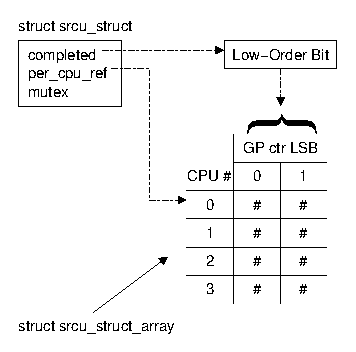
\includegraphics{appendix/rcuimpl/srcuds}}
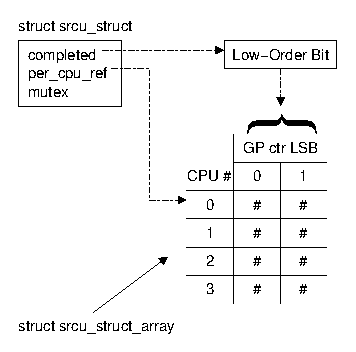
\includegraphics{appendix/rcuimpl/srcuds}
\end{center}
\caption{SRCU Data-Structure Diagram}
\label{fig:app:whymb:SRCU Data-Structure Diagram}
\end{figure}

\subsubsection{Initialization Implementation}
\label{sec:app:rcuimpl:Initialization Implementation}

SRCU's initialization function, \url{init_srcu_struct()}, is shown in
Figure~\ref{fig:app:rcuimpl:SRCU Initialization}.
This function simply initializes the fields in the
\url{struct} \url{srcu_struct}, returning zero if initialization succeeds
or \url{-ENOMEM} otherwise.

\begin{figure}[htbp]
{ \scriptsize
\begin{verbatim}
  1 int init_srcu_struct(struct srcu_struct *sp)
  2 {
  3   sp->completed = 0;
  4   mutex_init(&sp->mutex);
  5   sp->per_cpu_ref =
  6     alloc_percpu(struct srcu_struct_array);
  7   return (sp->per_cpu_ref ? 0 : -ENOMEM);
  8 }
\end{verbatim}
}
\caption{SRCU Initialization}
\label{fig:app:rcuimpl:SRCU Initialization}
\end{figure}

SRCU's cleanup functions are shown in
Figure~\ref{fig:app:rcuimpl:SRCU Cleanup}.
The main cleanup function, \url{cleanup_srcu_struct()} is shown
on lines~19-29 of this figure, however, it immediately invokes
\url{srcu_readers_active()}, shown on lines~13-17 of this figure,
to verify that there are no readers currently using this
\url{struct} \url{srcu_struct}.

The \url{srcu_readers_active()} function simply returns the sum of
\url{srcu_readers_active_idx()} on both possible indexes,
while \url{srcu_readers_active_idx()}, as shown on lines~1-11,
sums up the per-CPU counters corresponding to the specified index,
returning the result.

If the value returned from \url{srcu_readers_active()} is non-zero,
then \url{cleanup_srcu_struct()} issues a warning on line~24 and
simply returns on lines~25 and 26, declining to destroy a
\url{struct} \url{srcu_struct} that is still in use.
Such a warning always indicates a bug, and given that the bug
has been reported, it is better to allow the system to continue
with a modest memory leak than to introduce possible memory corruption.

Otherwise, \url{cleanup_srcu_struct()} frees the array of per-CPU
counters and \url{NULL}s the pointer on lines~27 and 28.

\begin{figure}[htbp]
{ \scriptsize
\begin{verbatim}
  1 int srcu_readers_active_idx(struct srcu_struct *sp,
  2                             int idx)
  3 {
  4   int cpu;
  5   int sum;
  6
  7   sum = 0;
  8   for_each_possible_cpu(cpu)
  9     sum += per_cpu_ptr(sp->per_cpu_ref, cpu)->c[idx];
 10   return sum;
 11 }
 12
 13 int srcu_readers_active(struct srcu_struct *sp)
 14 {
 15   return srcu_readers_active_idx(sp, 0) +
 16          srcu_readers_active_idx(sp, 1);
 17 }
 18
 19 void cleanup_srcu_struct(struct srcu_struct *sp)
 20 {
 21   int sum;
 22
 23   sum = srcu_readers_active(sp);
 24   WARN_ON(sum);
 25   if (sum != 0)
 26     return;
 27   free_percpu(sp->per_cpu_ref);
 28   sp->per_cpu_ref = NULL;
 29 }
\end{verbatim}
}
\caption{SRCU Cleanup}
\label{fig:app:rcuimpl:SRCU Cleanup}
\end{figure}

\subsubsection{Read-Side Implementation}
\label{sec:app:rcuimpl:Read-Side Implementation}

The code implementing \url{srcu_read_lock()} is shown in
Figure~\ref{fig:app:rcuimpl:Read-Side Acquisition}.
This function has been carefully constructed to avoid the
need for memory barriers and atomic instructions.

Lines~4 and 11 disable and re-enable preemption, in order to force
the sequence of code to execute unpreempted on a single CPU.
Line~6 picks up the bottom bit of the grace-period counter, which will
be used to select which rank of per-CPU counters is to be used for this
SRCU read-side critical section.
The \url{barrier()} call on line~7 is a directive to the compiler
that ensures that the index is
fetched but once,\footnote{
	Please note that, despite the name, \url{barrier()}
	has absolutely no effect on the CPU's ability to
	reorder execution of both code and of memory accesses.}
so that the index used on line~9 is the same
one returned on line~12.
Lines~8-9 increment the selected counter for the current CPU.\footnote{
	It is important to note that the \url{smp_processor_id()} primitive
	has long-term meaning only if preemption is disabled.
	In absence of preemption disabling, a potential preemption
	immediately following execution of this primitive could
	cause the subsequent code to execute on some other CPU.}
Line~10 forces subsequent execution to occur \emph{after}
lines~8-9, in order to prevent to misordering of any code
in a non-\url{CONFIG_PREEMPT} build, but only
from the perspective of an intervening interrupt handler.
However, in a \url{CONFIG_PREEMPT} kernel, the required \url{barrier()}
call is embedded in the \url{preempt_enable()} on line~11, so the
\url{srcu_barrier()} is a no-op in that case.
Finally, line~12 returns the index so that it may be passed in to the
corresponding \url{srcu_read_unlock()}.

\begin{figure}[htbp]
{ \scriptsize
\begin{verbatim}
  1 int srcu_read_lock(struct srcu_struct *sp)
  2 {
  3   int idx;
  4
  5   preempt_disable();
  6   idx = sp->completed & 0x1;
  7   barrier();
  8   per_cpu_ptr(sp->per_cpu_ref,
  9               smp_processor_id())->c[idx]++;
 10   srcu_barrier();
 11   preempt_enable();
 12   return idx;
 13 }
\end{verbatim}
}
\caption{SRCU Read-Side Acquisition}
\label{fig:app:rcuimpl:Read-Side Acquisition}
\end{figure}

The code for \url{srcu_read_unlock()} is shown in
Figure~\ref{fig:app:rcuimpl:Read-Side Release}.
Again, lines~3 and 7 disable and re-enable preemption so that the
whole code sequence executes unpreempted on a single CPU.
In \url{CONFIG_PREEMPT} kernels, the \url{preempt_disable()} on line~3
contains a \url{barrier()} primitive, otherwise, the \url{barrier()}
is supplied by line~4.
Again, this directive forces the subsequent code to execute after
the critical section from the perspective of intervening
interrupt handlers.
Lines~5 and 6 decrement the counter for this CPU, but with the same
index as was used by the corresponding \url{srcu_read_lock()}.

\begin{figure}[htbp]
{ \scriptsize
\begin{verbatim}
  1 void srcu_read_unlock(struct srcu_struct *sp, int idx)
  2 {
  3   preempt_disable();
  4   srcu_barrier();
  5   per_cpu_ptr(sp->per_cpu_ref,
  6               smp_processor_id())->c[idx]--;
  7   preempt_enable();
  8 }
\end{verbatim}
}
\caption{SRCU Read-Side Release}
\label{fig:app:rcuimpl:Read-Side Release}
\end{figure}

The key point is that the a given CPU's counters
can be observed by other CPUs only in
cooperation with that CPU's interrupt handlers.
These interrupt handlers are responsible for ensuring that any needed
memory barriers are executed prior to observing the counters.

\subsubsection{Update-Side Implementation}
\label{sec:app:rcuimpl:Update-Side Implementation}

The key point behind SRCU is that \url{synchronize_sched()}
blocks until all currently-executing preempt-disabled regions of
code complete.
The \url{synchronize_srcu()} primitive makes heavy use of this effect,
as can be seen in
Figure~\ref{fig:app:rcuimpl:Update-Side Implementation}.

Line~5 takes a snapshot of the grace-period counter.
Line~6 acquires the mutex, and lines~7-10 check to see whether
at least two grace periods have elapsed since the snapshot,
and, if so, releases the lock and returns --- in this case, someone
else has done our work for us.
Otherwise, line~11 guarantees that any other CPU that sees the
incremented value of the grace period counter in \url{srcu_read_lock()}
also sees any changes made by this CPU prior to entering
\url{synchronize_srcu()}.
This guarantee is required to make sure that any SRCU read-side
critical sections not blocking the next grace period have seen
any prior changes.

Line~12 fetches the bottom bit of the grace-period counter for later
use as an index into the per-CPU counter arrays, and then line~13
increments the grace-period counter.
Line~14 then waits for any currently-executing \url{srcu_read_lock()}
to complete, so that by the time that we reach line~15, all
extant instances of \url{srcu_read_lock()} will be using the updated
value from \url{sp->completed}.
Therefore, the counters sampled in by \url{srcu_readers_active_idx()}
on line~15 are guaranteed to
be monotonically decreasing, so that once their sum reaches zero, it
is guaranteed to stay there.

However, there are no memory barriers in the \url{srcu_read_unlock()}
primitive, so the CPU is within its rights to reorder the counter
decrement up into the SRCU critical section, so that references to
an SRCU-protected data structure could in effect ``bleed out'' of the
SRCU critical section.
This scenario is addressed by the \url{synchronize_sched()} on line~17,
which blocks until all other CPUs executing in \url{preempt_disable()}
code sequences (such as that in \url{srcu_read_unlock()}) complete these
sequences.
Because completion of a given \url{preempt_disable()} code sequence
is observed from the CPU executing that sequence, completion of the
sequence implies completion of any prior SRCU read-side critical section.
Any required memory barriers are supplied by the code making the
observation.

At this point, it is therefore safe to release the mutex as shown
on line~18 and return to the caller, who can now be assured that
all SRCU read-side critical sections sharing the same
\url{struct} \url{srcu_struct}
will observe any update made prior to the call to \url{synchronize_srcu()}.

\begin{figure}[htbp]
{ \scriptsize
\begin{verbatim}
  1 void synchronize_srcu(struct srcu_struct *sp)
  2 {
  3   int idx;
  4
  5   idx = sp->completed;
  6   mutex_lock(&sp->mutex);
  7   if ((sp->completed - idx) >= 2) {
  8     mutex_unlock(&sp->mutex);
  9     return;
 10   }
 11   synchronize_sched();
 12   idx = sp->completed & 0x1;
 13   sp->completed++;
 14   synchronize_sched();
 15   while (srcu_readers_active_idx(sp, idx))
 16     schedule_timeout_interruptible(1);
 17   synchronize_sched();
 18   mutex_unlock(&sp->mutex);
 19 }
\end{verbatim}
}
\caption{SRCU Update-Side Implementation}
\label{fig:app:rcuimpl:Update-Side Implementation}
\end{figure}

\QuickQuiz{}
	Why is it OK to assume that updates separated by
	{\tt synchronize\_sched()} will be performed in order?
\QuickQuizAnswer{
	Because this property is required for the {\tt synchronize\_sched()}
	aspect of RCU to work at all.
	For example, consider a code sequence that removes an object
	from a list, invokes {\tt synchronize\_sched()}, then frees
	the object.
	If this property did not hold, then that object might appear
	to be freed before it was
	removed from the list, which is precisely the situation that
	{\tt synchronize\_sched()} is supposed to prevent!
} \QuickQuizEnd

\QuickQuiz{}
	Why must line~17 in {\tt synchronize\_srcu()}
	(Figure~\ref{fig:app:rcuimpl:Update-Side Implementation})
	precede the release of the mutex on line~18?
	What would have to change to permit these two lines to be
	interchanged?
	Would such a change be worthwhile?
	Why or why not?
\QuickQuizAnswer{
	Suppose that the order was reversed, and that CPU~0
	has just reached line~13 of
	{\tt synchronize\_srcu()}, while both CPU~1 and CPU~2 start executing
	another {\tt synchronize\_srcu()} each, and CPU~3 starts executing a
	{\tt srcu\_read\_lock()}.
	Suppose that CPU~1 reaches line~6 of {\tt synchronize\_srcu()}
	just before CPU~0 increments the counter on line~13.
	Most importantly, suppose that
	CPU~3 executes {\tt srcu\_read\_lock()}
	out of order with the following SRCU read-side critical section,
	so that it acquires a reference to some SRCU-protected data
	structure \emph{before} CPU~0 increments {\tt sp->completed}, but
	executes the {\tt srcu\_read\_lock()} \emph{after} CPU~0 does
	this increment.
	
	Then CPU~0 will \emph{not} wait for CPU~3 to complete its
	SRCU read-side critical section before exiting the ``while''
	loop on lines~15-16 and releasing the mutex (remember, the
	CPU could be reordering the code).
	
	Now suppose that CPU~2 acquires the mutex next,
	and again increments {\tt sp->completed}.
	This CPU will then have to wait for CPU~3 to exit its SRCU
	read-side critical section before exiting the loop on
	lines~15-16 and releasing the mutex.
	But suppose that CPU~3 again executes out of order,
	completing the {\tt srcu\_read\_unlock()} prior to
	executing a final reference to the pointer it obtained
	when entering the SRCU read-side critical section.

	CPU~1 will then acquire the mutex, but see that the
	{\tt sp->completed} counter has incremented twice, and
	therefore take the early exit.
	The caller might well free up the element that CPU~3 is
	still referencing (due to CPU~3's out-of-order execution).

	To prevent this perhaps improbable, but entirely possible,
	scenario, the final {\tt synchronize\_sched()} must precede
	the mutex release in {\tt synchronize\_srcu()}.

	Another approach would be to change to comparison on
	line~7 of {\tt synchronize\_srcu()} to check for at
	least three increments of the counter.
	However, such a change would increase the latency of a
	``bulk update'' scenario, where a hash table is being updated
	or unloaded using multiple threads.
	In the current code, the latency of the resulting concurrent
	{\tt synchronize\_srcu()} calls would take at most two SRCU
	grace periods, while with this change, three would be required.

	More experience will be required to determine which approach
	is really better.
	For one thing, there must first be some use of SRCU with
	multiple concurrent updaters.
} \QuickQuizEnd

\subsection{SRCU Summary}
\label{sec:app:rcuimpl:SRCU Summary}

SRCU provides an RCU-like set of primitives that permit general
sleeping in the SRCU read-side critical sections.
However, it is important to note that SRCU has been used only in
prototype code, though it has passed the RCU torture test.
It will be very interesting to see what use, if any, SRCU sees
in the future.

% \input{appendix/rcuimpl/rcuclassic.tex}  @@@ from Ph.D. dissertation.
% appendix/rcuimpl/rcutree.tex

\section{Hierarchical RCU Overview}
\label{app:rcuimpl:rcutree:Hierarchical RCU Overview}

Although Classic RCU's read-side primitives enjoy excellent
performance and scalability, the update-side primitives, which
determine when pre-existing read-side critical sections have
finished, were designed with only a few tens of CPUs in mind.
Their scalability is limited by a global lock that must be
acquired by each CPU at least once during each grace period.
Although Classic RCU actually scales to a couple of hundred CPUs, and
can be tweaked to scale to roughly a thousand CPUs (but at the expense of
extending grace periods), emerging multicore systems will require
it to scale better.

In addition, Classic RCU has a sub-optimal dynticks interface,
with the result that Classic RCU will wake up every CPU at least
once per grace period.
To see the problem with this, consider a 16-CPU system that
is sufficiently lightly loaded that it is keeping only four
CPUs busy.
In a perfect world, the remaining twelve CPUs could be put into
deep sleep mode in order to conserve energy.
Unfortunately, if the four busy CPUs are frequently performing
RCU updates, those twelve idle CPUs will be awakened frequently,
wasting significant energy.
Thus, any major change to Classic RCU should also leave sleeping CPUs lie.

Both the classic and the hierarchical implementations
have have Classic RCU semantics and identical APIs, however,
the old implementation will be called ``classic RCU''
and the new implementation will be called ``hierarchical RCU''.

@@@ roadmap @@@

\subsection{Review of RCU Fundamentals}
\label{app:rcuimpl:rcutree:Review of RCU Fundamentals}

In its most basic form, RCU is a way of waiting for things to finish.
Of course, there are a great many other ways of waiting for things to
finish, including reference counts, reader-writer locks, events, and so on.
The great advantage of RCU is that it can wait for each of
(say) 20,000 different things without having to explicitly
track each and every one of them, and without having to worry about
the performance degradation, scalability limitations, complex deadlock
scenarios, and memory-leak hazards that are inherent in schemes
using explicit tracking.

In RCU's case, the things waited on are called
"RCU read-side critical sections".
An RCU read-side critical section starts with an
\url{rcu_read_lock()} primitive, and ends with a corresponding
\url{rcu_read_unlock()} primitive.
RCU read-side critical sections can be nested, and may contain pretty
much any code, as long as that code does not explicitly block or sleep
(although a special form of RCU called SRCU, described in
Section~\ref{app:rcuimpl:Sleepable RCU Implementation}
does permit general sleeping in SRCU read-side critical sections).
If you abide by these conventions, you can use RCU to wait for \emph{any}
desired piece of code to complete.

RCU accomplishes this feat by indirectly determining when these
other things have finished, as has been described in
@@@ ref @@@
for classic RCU and
Section~\ref{app:rcuimpl:Preemptable RCU} for preemptable RCU.

In particular, as shown in the
Figure~\ref{fig:defer:Readers and RCU Grace Period} on
page~\ref{fig:defer:Readers and RCU Grace Period},
RCU is a way of
waiting for pre-existing RCU read-side critical sections to completely
finish, also including the memory operations executed
by those critical sections.

However, note that RCU read-side critical sections
that begin after the beginning
of a given grace period can and will extend beyond the end of that grace
period.

The following section gives a very high-level view of how
the Classic RCU implementation operates.

\subsection{Brief Overview of Classic RCU Implementation}
\label{app:rcuimpl:rcutree:Brief Overview of Classic RCU Implementation}

@@@ redundant? @@@

The key concept behind the Classic RCU implementation is that
Classic RCU read-side critical sections are confined to kernel
code and are not permitted to block.
This means that any time a given CPU is seen
either blocking, in the idle loop, or exiting the kernel, we know that all
RCU read-side critical sections that were previously running on
that CPU must have completed.
Such states are called ``quiescent states'', and
after each CPU has passed through at least one quiescent state,
the RCU grace period ends.

\begin{figure}[htb]
\begin{center}
\resizebox{3in}{!}{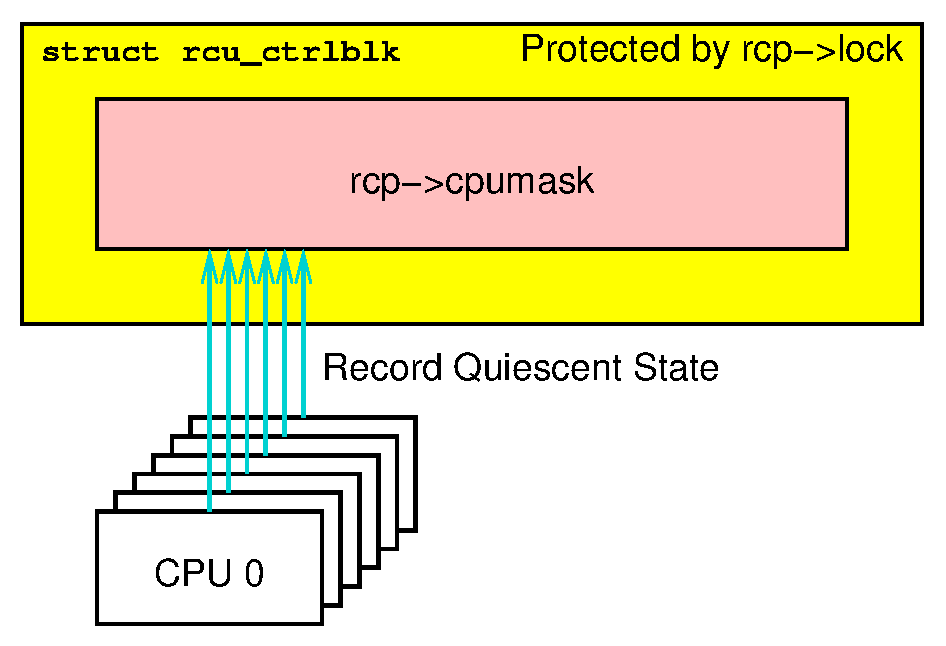
\includegraphics{appendix/rcuimpl/FlatClassicRCU}}
\end{center}
\caption{Flat Classic RCU State}
\label{fig:app:rcuimpl:rcutree:Flat Classic RCU State}
\end{figure}

Classic RCU's most important data structure is the \url{rcu_ctrlblk}
structure, which contains the \url{->cpumask} field, which contains
one bit per CPU, as shown in
Figure~\ref{fig:app:rcuimpl:rcutree:Flat Classic RCU State}.
Each CPU's bit is set to one at the beginning of each grace period,
and each CPU must clear its bit after it passes through a quiescent
state.
Because multiple CPUs might want to clear their bits concurrently,
which would corrupt the \url{->cpumask} field, a
\url{->lock} 
spinlock is used to protect \url{->cpumask}, preventing any
such corruption.
Unfortunately, this spinlock can also suffer extreme contention if there
are more than a few hundred CPUs, which might soon become quite common
if multicore trends continue.
Worse yet, the fact that \emph{all} CPUs must clear their own bit means
that CPUs are not permitted to sleep through a grace period, which limits
Linux's ability to conserve power.




The next section lays out what we need from a new non-real-time
RCU implementation.

\subsection{RCU Desiderata}
\label{app:rcuimpl:rcutree:RCU Desiderata}

The list of real-time RCU desiderata~\cite{PaulMcKenney05b}
is a very good start:

\begin{enumerate}
\item	Deferred destruction, so that an RCU grace period cannot end
	until all pre-existing RCU read-side critical sections have
	completed.
\item	Reliable, so that RCU supports 24x7 operation for years at
	a time.
\item	Callable from irq handlers.
\item	Contained memory footprint, so that mechanisms exist to expedite
	grace periods if there are too many callbacks.  (This is weakened
	from the LCA2005 list.)
\item	Independent of memory blocks, so that RCU can work with any
	conceivable memory allocator.
\item	Synchronization-free read side, so that only normal non-atomic
	instructions operating on CPU- or task-local memory are permitted.
	(This is strengthened from the LCA2005 list.)
\item	Unconditional read-to-write upgrade, which is used in several
	places in the Linux kernel where the update-side lock is
	acquired within the RCU read-side critical section.
\item	Compatible API.

\item	Because this is not to be a real-time RCU, the requirement for
	preemptable RCU read-side critical sections can be dropped.
	However, we need to add the following new requirements to account
	for changes over the past few years.

\item	Scalability with extremely low internal-to-RCU lock contention.
	RCU must support at least 1,024 CPUs gracefully, and preferably
	at least 4,096.
\item	Energy conservation: RCU must be able to avoid awakening
	low-power-state dynticks-idle CPUs, but still determine
	when the current grace period ends.
	This has been implemented in real-time RCU, but needs serious
	simplification.
\item	RCU read-side critical sections must be permitted in NMI
	handlers as well as irq handlers.  Note that preemptable RCU
	was able to avoid this requirement due to a separately
	implemented \url{synchronize_sched()}.
\item	RCU must operate gracefully in face of repeated CPU-hotplug
	operations.
	This is simply carrying forward a requirement met by both
	classic and real-time.
\item	It must be possible to wait for all previously registered
	RCU callbacks to complete, though this is already provided
	in the form of \url{rcu_barrier()}.
\item	Detecting CPUs that are failing to respond is desirable,
	to assist diagnosis both of RCU and of various infinite
	loop bugs and hardware failures that can prevent RCU grace
	periods from ending.
\item	Extreme expediting of RCU grace periods is desirable,
	so that an RCU grace period can be forced to complete within
	a few hundred microseconds of the last relevant RCU read-side
	critical second completing.
	However, such an operation would be expected to incur
	severe CPU overhead, and would be primarily useful when
	carrying out a long sequence of operations that each needed
	to wait for an RCU grace period.
\end{enumerate}

The most pressing of the new requirements is the first one, scalability.
The next section therefore describes how to make order-of-magnitude reductions
in contention on RCU's internal locks.

\subsection{Towards a More Scalable RCU Implementation}
\label{app:rcuimpl:rcutree:Towards a More Scalable RCU Implementation}

\begin{figure}[htb]
\begin{center}
\resizebox{3in}{!}{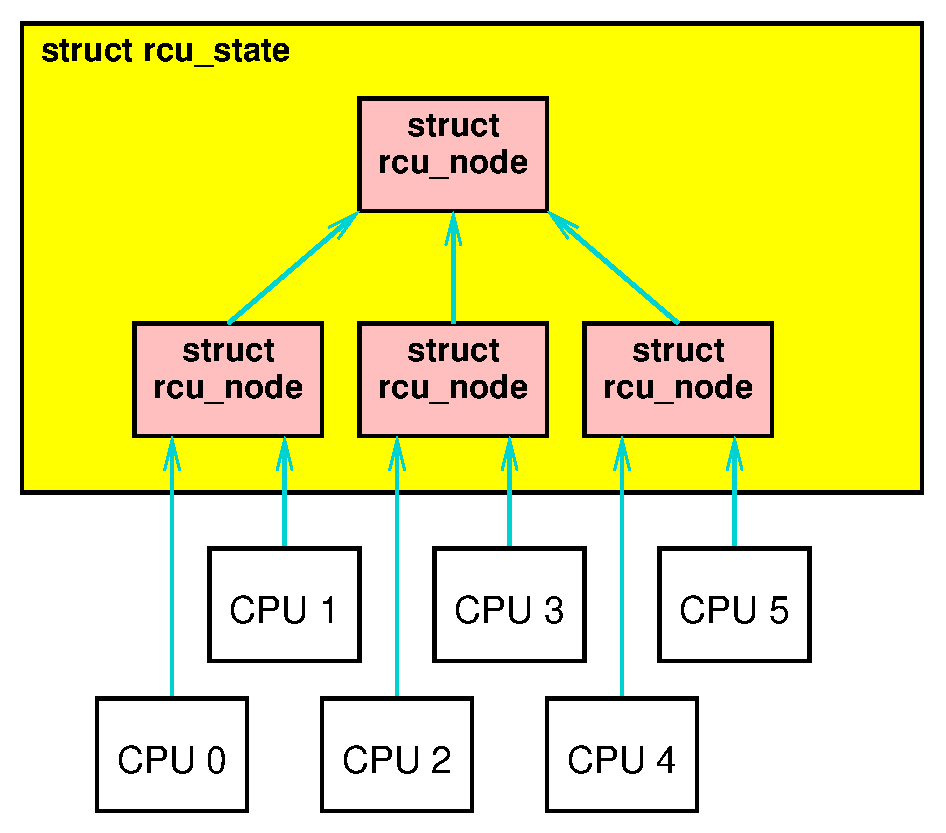
\includegraphics{appendix/rcuimpl/TreeClassicRCU}}
\end{center}
\caption{Hierarchical RCU State}
\label{fig:app:rcuimpl:rcutree:Hierarchical RCU State}
\end{figure}

One effective way to reduce lock contention is to create a hierarchy,
as shown in
Figure~\ref{fig:app:rcuimpl:rcutree:Hierarchical RCU State}.
Here, each of the four \url{rcu_node} structures has its own lock,
so that only CPUs~0 and 1 will acquire the lower left
\url{rcu_node}'s lock, only CPUs~2 and 3 will acquire the
lower middle \url{rcu_node}'s lock, and only CPUs~4 and 5
will acquire the lower right \url{rcu_node}'s lock.
During any given grace period,
only one of the CPUs accessing each of the lower \url{rcu_node}
structures will access the upper \url{rcu_node}, namely, the
last of each pair of CPUs to record a quiescent state for the corresponding
grace period.

This results in a significant reduction in lock contention:
instead of six CPUs contending for a single lock each grace period,
we have only three for the upper \url{rcu_node}'s lock 
(a reduction of 50\%) and only
two for each of the lower \url{rcu_node}s' locks (a reduction
of 67\%).

\begin{figure}[htb]
\begin{center}
\resizebox{3in}{!}{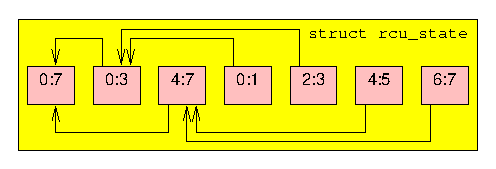
\includegraphics{appendix/rcuimpl/TreeMapping}}
\end{center}
\caption{Mapping {\tt rcu\_node} Hierarchy Into Array}
\label{fig:app:rcuimpl:rcutree:Mapping rcu-node Hierarchy Into Array}
\end{figure}

The tree of \url{rcu_node} structures is embedded into
a linear array in the \url{rcu_state} structure,
with the root of the tree in element zero, as shown in
Figure~\ref{fig:app:rcuimpl:rcutree:Mapping rcu-node Hierarchy Into Array}
for an eight-CPU
system with a three-level hierarchy.
Each arrow links a given \url{rcu_node} structure to its parent,
representing the \url{rcu_node}'s \url{->parent} field.
Each \url{rcu_node} indicates the range of CPUs covered,
so that the root node covers all of the CPUs, each node in the second
level covers half of the CPUs, and each node in the leaf level covering
a pair of CPUs.
This array is allocated statically at compile time based on the value
of \url{NR_CPUS}.

\begin{figure*}[htbp]
\begin{center}
\resizebox{3in}{!}{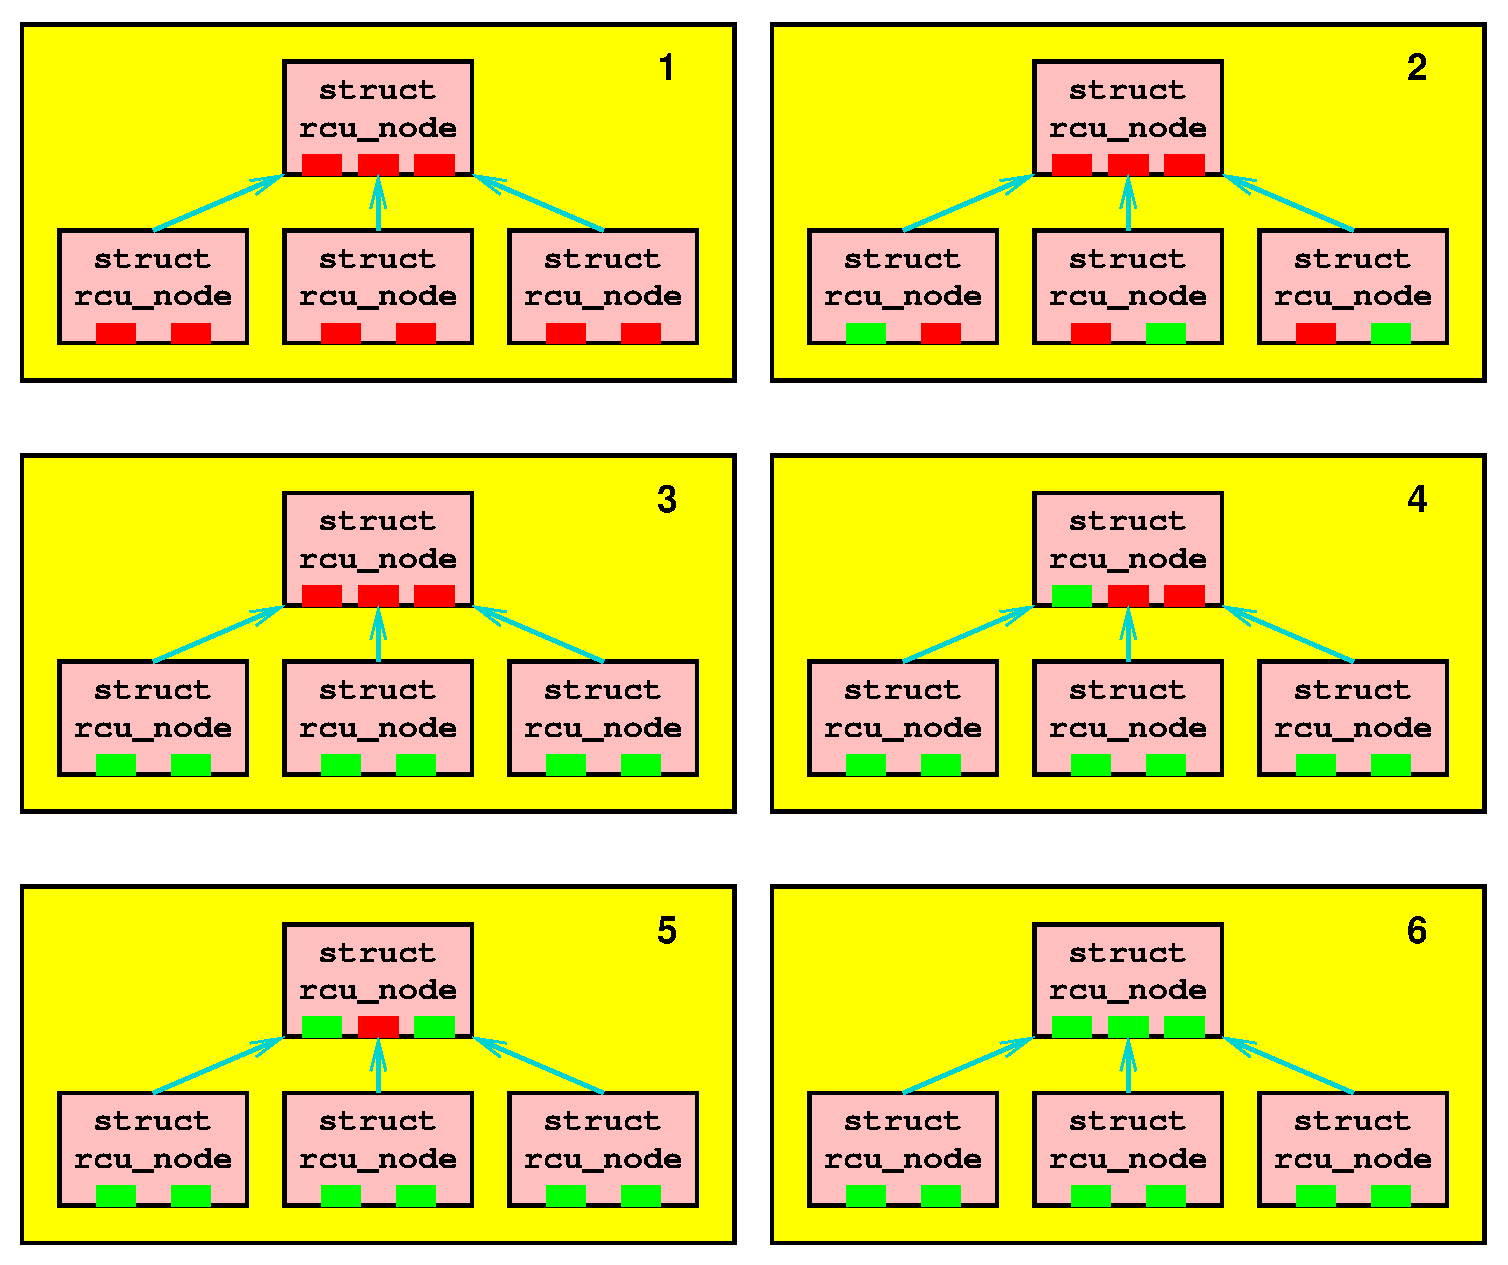
\includegraphics{appendix/rcuimpl/TreeClassicRCUGP}}
\end{center}
\caption{Hierarchical RCU Grace Period}
\label{fig:app:rcuimpl:rcutree:Hierarchical RCU Grace Period}
\end{figure*}

The sequence of diagrams in
Figure~\ref{fig:app:rcuimpl:rcutree:Hierarchical RCU Grace Period}
shows how grace periods are detected.
In the first figure, no CPU has yet passed through a quiescent state,
as indicated by the red rectangles.
Suppose that all six CPUs simultaneously try to tell RCU that they have
passed through a quiescent state.
Only one of each pair will be able to acquire the lock on the
corresponding lower \url{rcu_node}, and so the second figure
shows the result if the lucky CPUs are numbers 0, 3, and 5, as indicated
by the green rectangles.
Once these lucky CPUs have finished, then the other CPUs will acquire
the lock, as shown in the third figure.
Each of these CPUs will see that they are the last in their group,
and therefore all three will attempt to move to the upper
\url{rcu_node}.
Only one at a time can acquire the upper \url{rcu_node} structure's
lock, and the fourth, fifth, and sixth figures show the sequence of
states assuming that CPU~1, CPU~2, and CPU~4 acquire
the lock in that order.
The sixth and final figure in the group shows that all CPUs have passed
through a quiescent state, so that the grace period has ended.

\begin{figure}[htb]
\begin{center}
\resizebox{3in}{!}{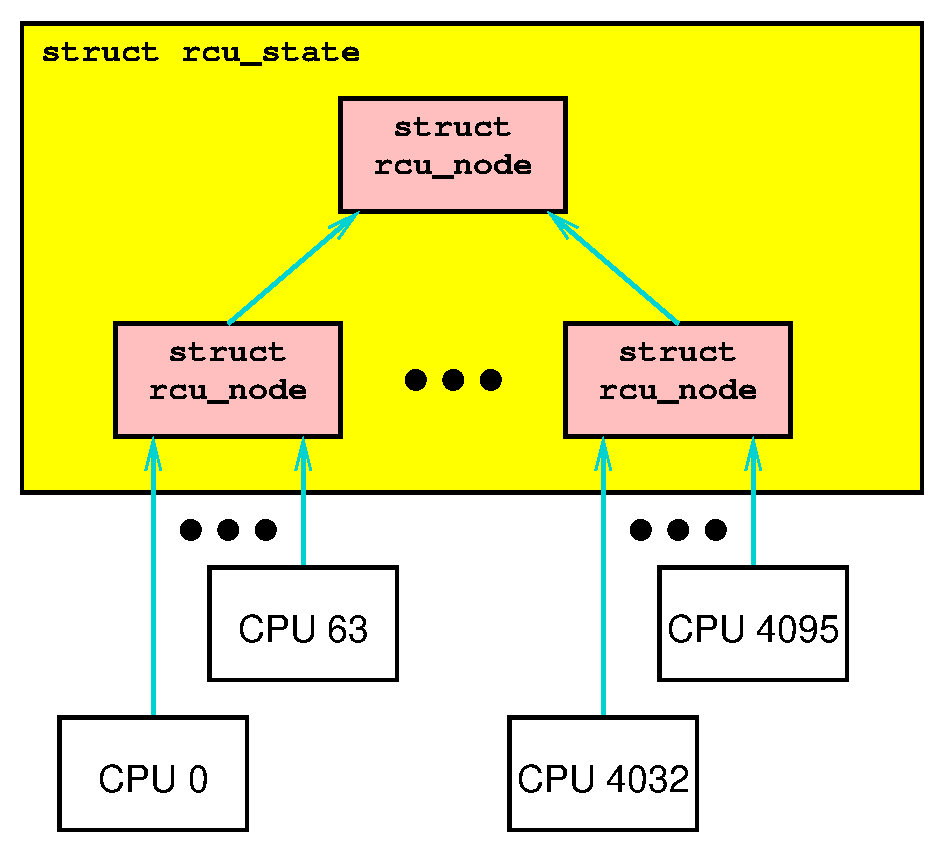
\includegraphics{appendix/rcuimpl/BigTreeClassicRCU}}
\end{center}
\caption{Hierarchical RCU State 4,096 CPUs}
\label{fig:app:rcuimpl:rcutree:Hierarchical RCU State 4,096 CPUs}
\end{figure}

In the above sequence, there were never more than three CPUs
contending for any one lock, in happy contrast to Classic RCU,
where all six CPUs might contend.
However, even more dramatic reductions in lock contention are
possible with larger numbers of CPUs.
Consider a hierarchy of \url{rcu_node} structures, with
64 lower structures and 64*64=4,096 CPUs, as shown in
Figure~\ref{fig:app:rcuimpl:rcutree:Hierarchical RCU State 4,096 CPUs}.

Here each of the lower \url{rcu_node} structures' locks
are acquired by 64 CPUs, a 64-times reduction from the 4,096 CPUs
that would acquire Classic RCU's single global lock.
Similarly, during a given grace period, only one CPU from each of
the lower \url{rcu_node} structures will acquire the
upper \url{rcu_node} structure's lock, which is again
a 64x reduction from the contention level that would be experienced
by Classic RCU running on a 4,096-CPU system.

\QuickQuiz{Wait a minute!  With all those new locks, how do you avoid deadlock?}
\QuickQuizAnswer{
Deadlock is avoided by never holding more than one of the
\url{rcu_node} structures' locks at a given time.
This algorithm uses two more locks, one to prevent CPU hotplug operations
from running concurrently with grace-period advancement
(\url{onofflock}) and another
to permit only one CPU at a time from forcing a quiescent state
to end quickly (\url{fqslock}).
These are subject to a locking hierarchy, so that
\url{fqslock} must be acquired before
\url{onofflock}, which in turn must be acquired before
any of the \url{rcu_node} structures' locks.

Also, as a practical matter, refusing to ever hold more than
one of the \url{rcu_node} locks means that it is unnecessary
to track which ones are held.
Such tracking would be painful as well as unnecessary.
} \QuickQuizEnd

\QuickQuiz{Why stop at a 64-times reduction?
Why not go for a few orders of magnitude instead?}
\QuickQuizAnswer{
RCU works with no problems on
systems with a few hundred CPUs, so allowing 64 CPUs to contend on
a single lock leaves plenty of headroom.
Keep in mind that these locks are acquired quite rarely, as each
CPU will check in about one time per grace period, and grace periods
extend for milliseconds.
} \QuickQuizEnd

\QuickQuiz{But I don't care about McKenney's lame excuses in the answer to
Quick Quiz 2!!!
I want to get the number of CPUs contending on a single lock down
to something reasonable, like sixteen or so!!!}
\QuickQuizAnswer{
OK, have it your way, then!!!
Set \url{CONFIG_RCU_FANOUT=16} and (for \url{NR_CPUS=4096})
you will get a
three-level hierarchy with with 256 \url{rcu_node} structures
at the lowest level, 16 \url{rcu_node} structures as intermediate
nodes, and a single root-level \url{rcu_node}.
The penalty you will pay is that more \url{rcu_node} structures
will need to be scanned when checking to see which CPUs need help
completing their quiescent states (256 instead of only 64).
} \QuickQuizEnd

\begin{figure}[htb]
\begin{center}
\resizebox{3in}{!}{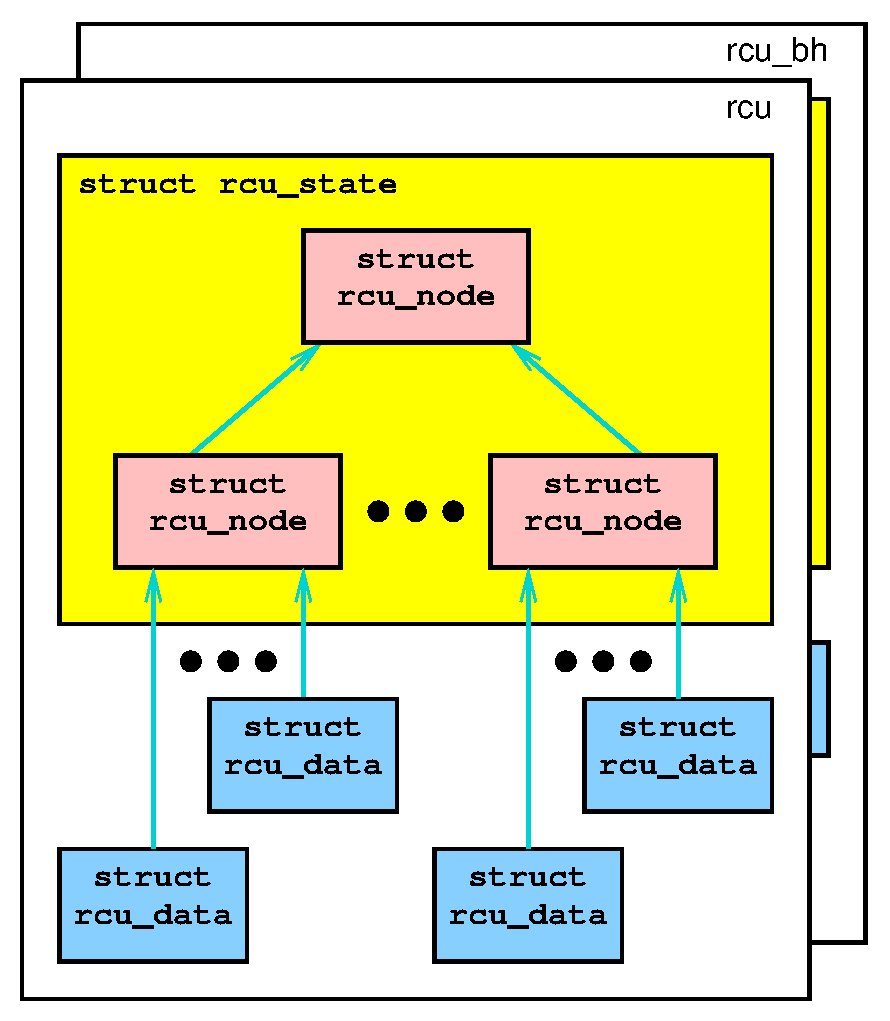
\includegraphics{appendix/rcuimpl/BigTreeClassicRCUBH}}
\end{center}
\caption{Hierarchical RCU State With BH}
\label{fig:app:rcuimpl:rcutree:Hierarchical RCU State With BH}
\end{figure}

The implementation maintains some per-CPU data, such as lists of
RCU callbacks, organized into \url{rcu_data} structures.
In addition, rcu (as in \url{call_rcu()}) and
rcu\_bh (as in \url{call_rcu_bh()}) each maintain their own
hierarchy, as shown in
Figure~\ref{fig:app:rcuimpl:rcutree:Hierarchical RCU State With BH}.

\QuickQuiz{OK, so what is the story with the colors?}
\QuickQuizAnswer{
Data structures analogous to \url{rcu_state} (including
\url{rcu_ctrlblk}) are yellow,
those containing the bitmaps used to determine when CPUs have checked
in are pink,
and the per-CPU \url{rcu_data} structures are blue.
The data structures used to conserve energy
(such as \url{rcu_dynticks}) will be colored green.
} \QuickQuizEnd

The next section discusses energy conservation.

\subsection{Towards a Greener RCU Implementation}
\label{app:rcuimpl:rcutree:Towards a Greener RCU Implementation}

As noted earlier, an important goal of this effort is to leave sleeping
CPUs lie in order to promote energy conservation.
In contrast, classic RCU will happily awaken each and every sleeping CPU
at least once per grace period in some cases,
which is suboptimal in the case where
a small number of CPUs are busy doing RCU updates and the majority of
the CPUs are mostly idle.
This situation occurs frequently in systems sized for peak loads, and
we need to be able to accommodate it gracefully.
Furthermore, we need to fix a long-standing bug in Classic RCU where
a dynticks-idle CPU servicing an interrupt containing a long-running
RCU read-side critical section will fail to prevent an RCU grace period
from ending.

\QuickQuiz{Given such an egregious bug, why does Linux run at all?}
\QuickQuizAnswer{
Because the Linux kernel contains device drivers that are (relatively)
well behaved.
Few if any of them spin in RCU read-side critical sections for the
many milliseconds that would be required to provoke this bug.
The bug nevertheless does need to be fixed, and this variant of
RCU does fix it.
} \QuickQuizEnd

\begin{figure}[htb]
\begin{center}
\resizebox{3in}{!}{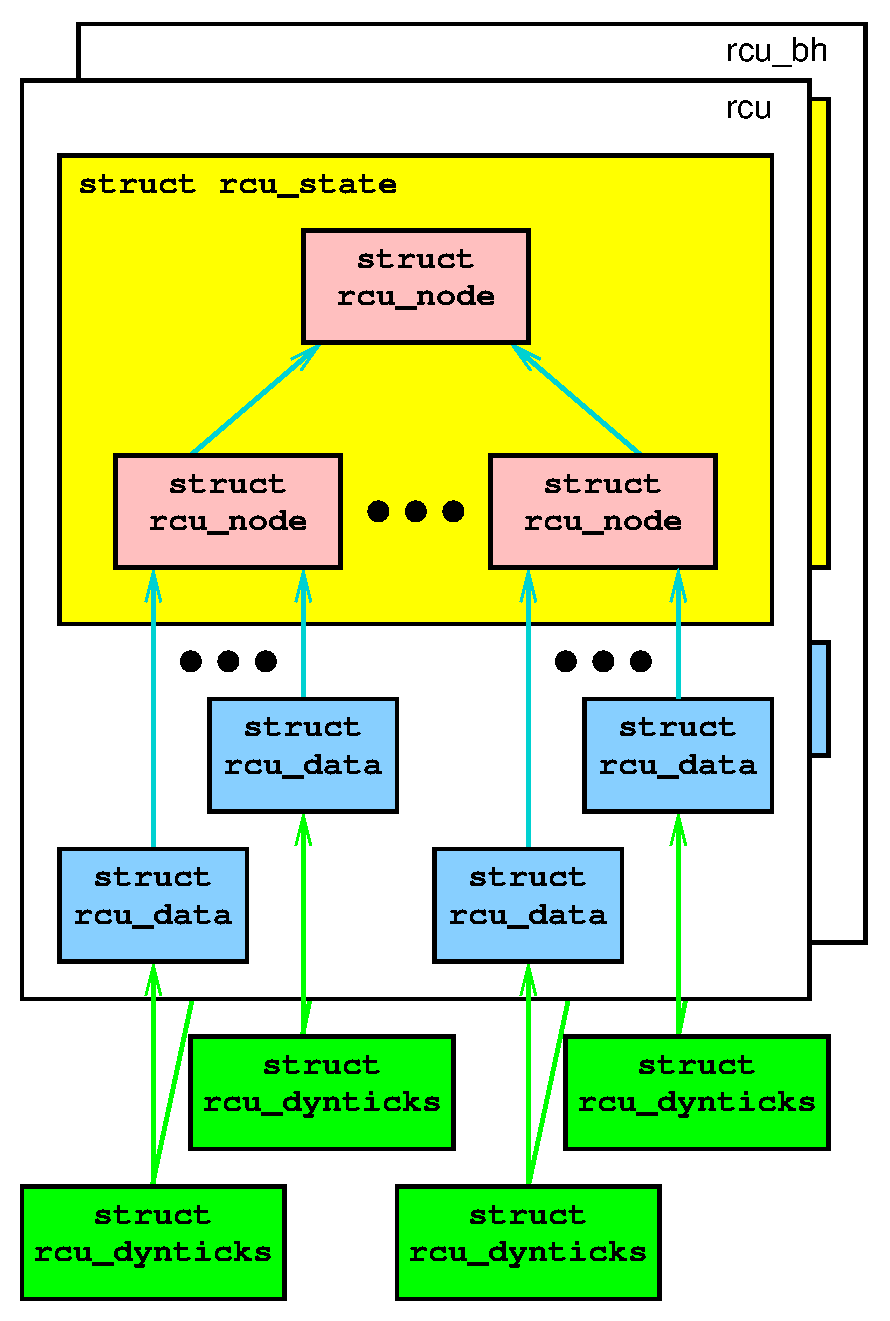
\includegraphics{appendix/rcuimpl/BigTreeClassicRCUBHdyntick}}
\end{center}
\caption{Hierarchical RCU State With Dynticks}
\label{fig:app:rcuimpl:rcutree:Hierarchical RCU State With Dynticks}
\end{figure}

This is accomplished by requiring that all CPUs manipulate counters
located in a per-CPU \url{rcu_dynticks} structure.
Loosely speaking, these counters have even-numbered values when the
corresponding CPU is in dynticks idle mode, and have odd-numbered values
otherwise.
RCU thus needs to wait for quiescent states only for those CPUs whose
\url{rcu_dynticks} counters are odd, and need not wake up sleeping
CPUs, whose counters will be even.
As shown in
Figure~\ref{fig:app:rcuimpl:rcutree:Hierarchical RCU State With Dynticks},
each per-CPU \url{rcu_dynticks} structure
is shared by the ``rcu'' and ``rcu\_bh'' implementations.

The following section presents a high-level view of the RCU state machine.

\subsection{State Machine}
\label{app:rcuimpl:rcutree:State Machine}

\begin{figure}[htbp]
\begin{center}
\resizebox{3in}{!}{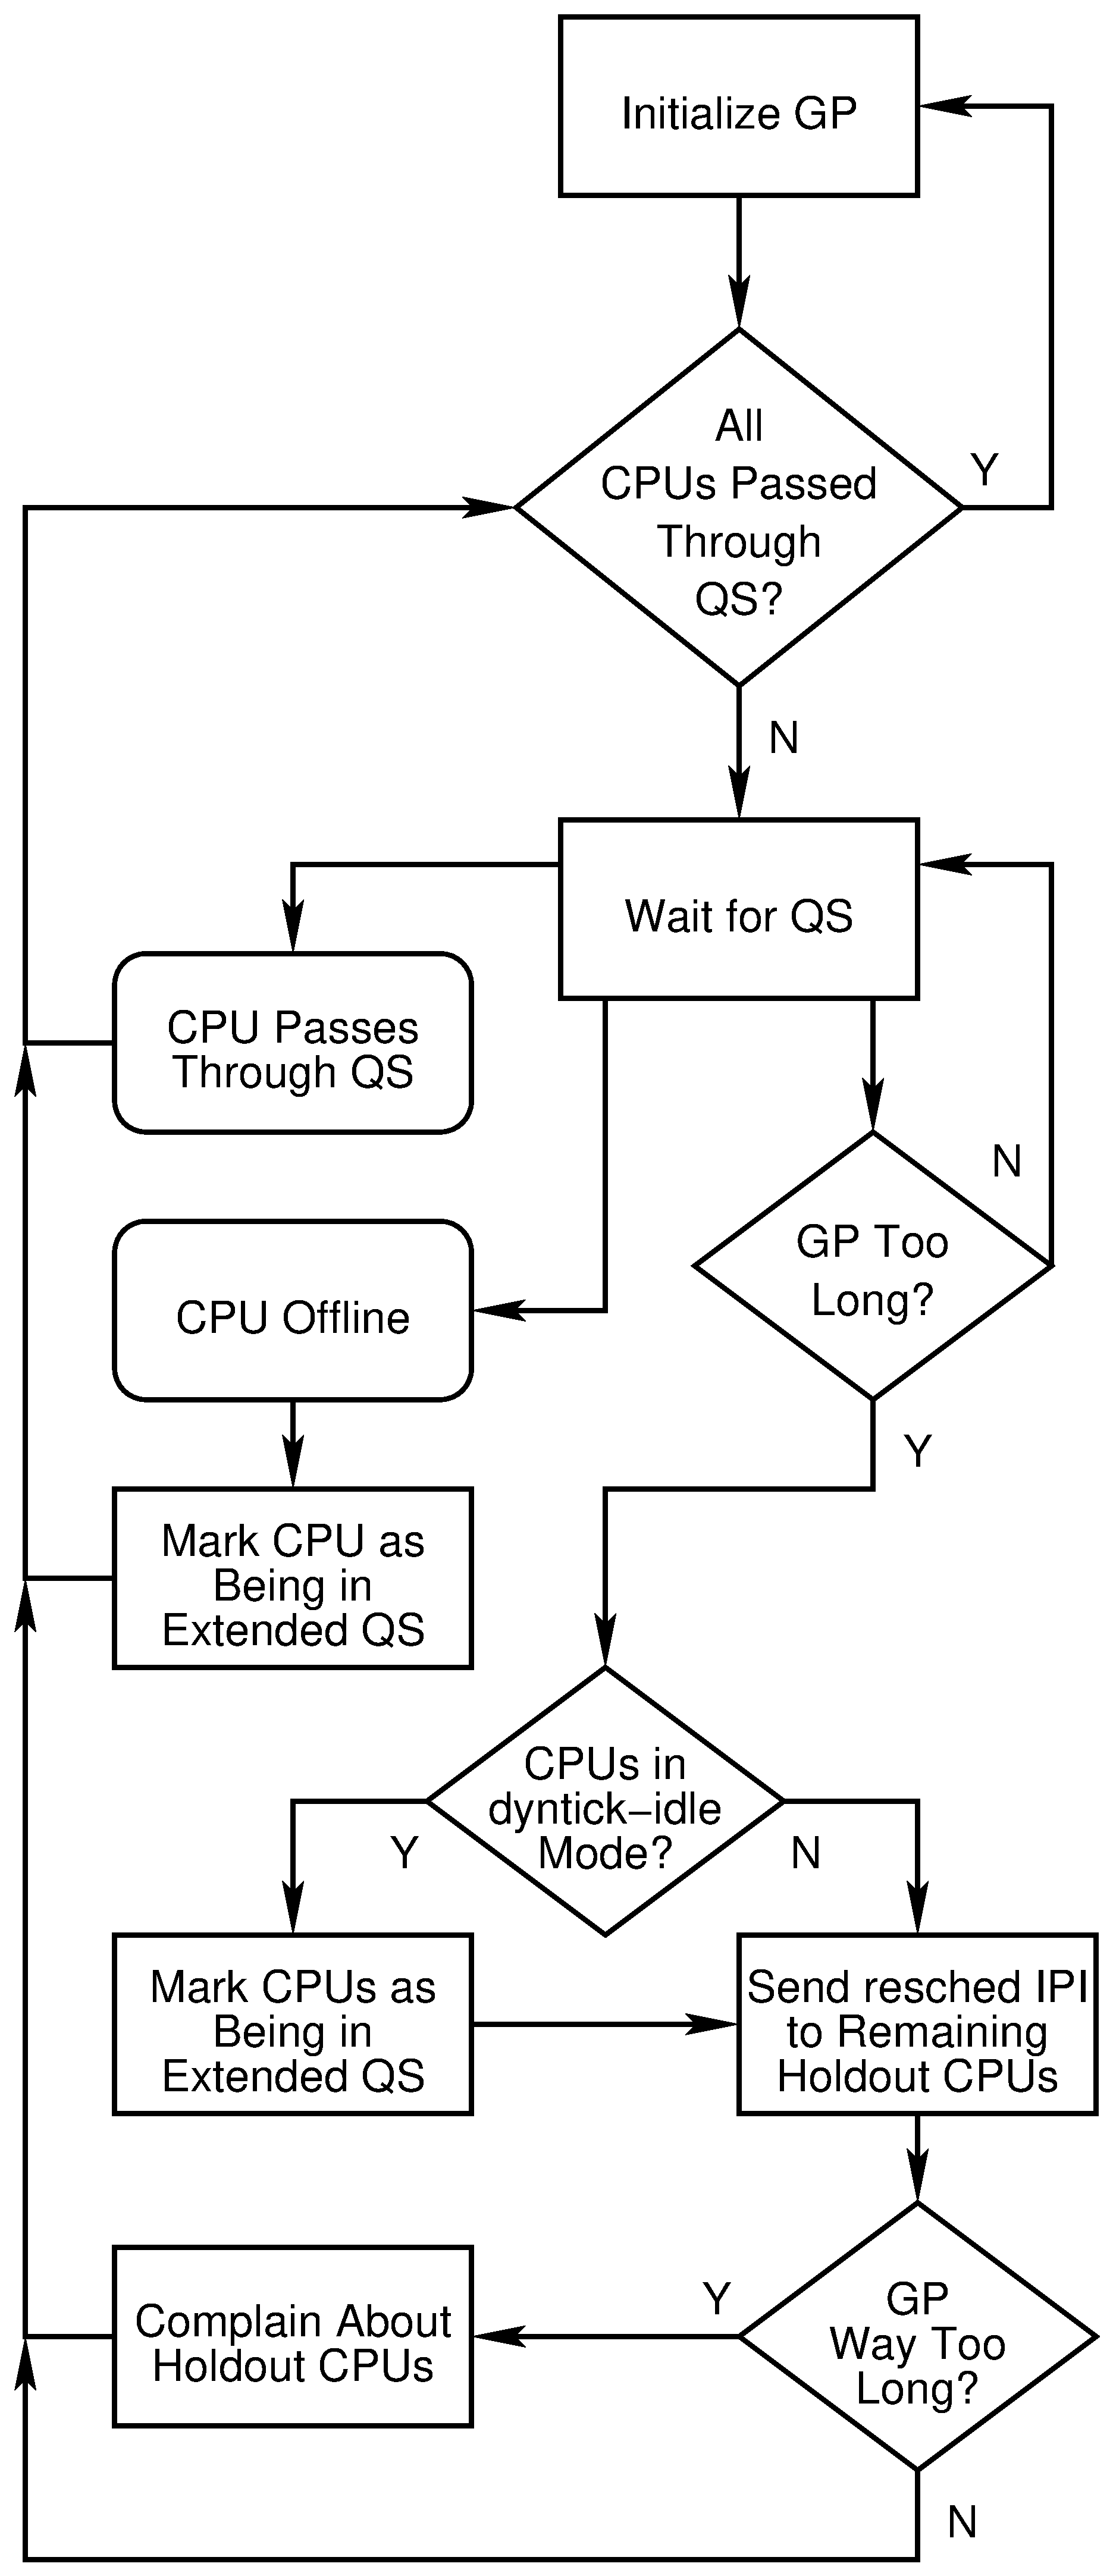
\includegraphics{appendix/rcuimpl/GenericRCUStateMachine}}
\end{center}
\caption{Generic RCU State Machine}
\label{fig:app:rcuimpl:rcutree:Generic RCU State Machine}
\end{figure}

At a sufficiently high level, Linux-kernel RCU implementations can
be thought of as high-level state machines as shown in
Figure~\ref{fig:app:rcuimpl:rcutree:Generic RCU State Machine}.
The common-case path through this state machine on a busy system
goes through the two uppermost loops, initializing at the
beginning of each grace period (GP),
waiting for quiescent states (QS), and noting when each CPU passes through
its first quiescent state for a given grace period.
On such a system, quiescent states will occur on each context switch,
or, for CPUs that are either idle or executing user-mode code, each
scheduling-clock interrupt.
CPU-hotplug events will take the state machine through the
``CPU Offline'' box, while the presence of ``holdout''
CPUs that fail to pass through quiescent states quickly enough will exercise
the path through the ``Send resched IPIs to Holdout CPUs'' box.
RCU implementations that avoid unnecessarily awakening dyntick-idle
CPUs will mark those CPUs as being in an extended quiescent state,
taking the ``Y'' branch out of the ``CPUs in dyntick-idle
Mode?'' decision diamond (but note that CPUs in dyntick-idle mode
will \emph{not} be sent resched IPIs).
Finally, if \url{CONFIG_RCU_CPU_STALL_DETECTOR} is enabled,
truly excessive delays in reaching quiescent states will exercise the
``Complain About Holdout CPUs'' path.

\QuickQuiz{But doesn't this state diagram indicate that dyntick-idle CPUs will
get hit with reschedule IPIs?  Won't that wake them up?}
\QuickQuizAnswer{
No.
Keep in mind that RCU is handling groups of CPUs.
One particular group might contain both dyntick-idle CPUs and
CPUs in normal mode that have somehow managed to avoid passing through
a quiescent state.
Only the latter group will be sent a reschedule IPI; the dyntick-idle
CPUs will merely be marked as being in an extended quiescent state.
} \QuickQuizEnd

\begin{figure}[htb]
\begin{center}
\resizebox{3in}{!}{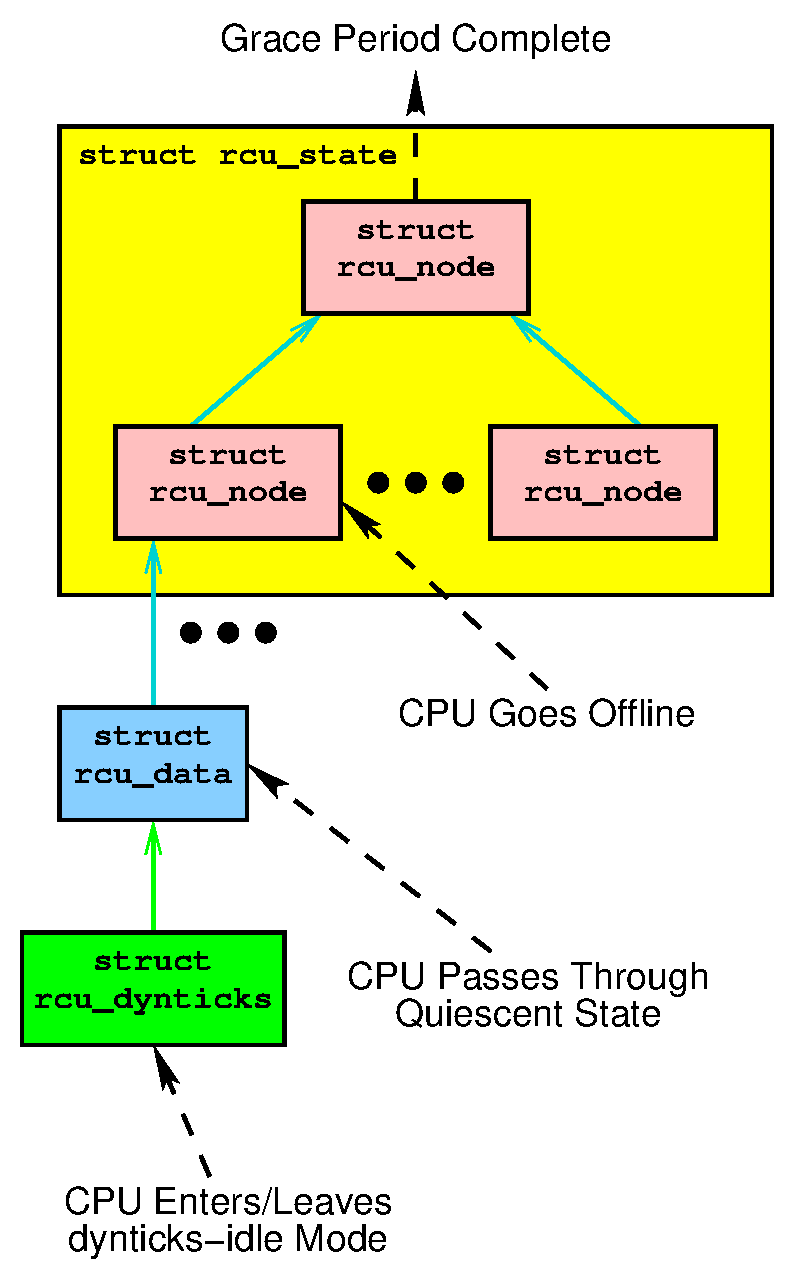
\includegraphics{appendix/rcuimpl/TreeRCUStateMachine}}
\end{center}
\caption{RCU State Machine and Hierarchical RCU Data Structures}
\label{fig:app:rcuimpl:rcutree:RCU State Machine and Hierarchical RCU Data Structures}
\end{figure}

The events in the above state schematic interact with different
data structures, as shown in
Figure~\ref{fig:app:rcuimpl:rcutree:RCU State Machine and Hierarchical RCU Data Structures}.
However, the state schematic does not directly translate into C code
for any of the RCU implementations.
Instead, these implementations are coded as an event-driven system within
the kernel.
Therefore, the following section describes some ``use cases'',
or ways in which the RCU algorithm traverses the above state schematic
as well as the relevant data structures.

\subsection{Use Cases}
\label{app:rcuimpl:rcutree:Use Cases}

This section gives an overview of several ``use cases''
within the RCU implementation, listing the data structures touched
and the functions invoked.
The use cases are as follows:

\begin{enumerate}
\item	Start a New Grace Period
	(Section~\ref{app:rcuimpl:rcutree:Start a New Grace Period})
\item	Pass Through a Quiescent State
	(Section~\ref{app:rcuimpl:rcutree:Pass Through a Quiescent State})
\item	Announce a Quiescent State to RCU
	(Section~\ref{app:rcuimpl:rcutree:Announce a Quiescent State to RCU})
\item	Enter and Leave Dynticks Idle Mode
	(Section~\ref{app:rcuimpl:rcutree:Enter and Leave Dynticks Idle Mode})
\item	Interrupt from Dynticks Idle Mode
	(Section~\ref{app:rcuimpl:rcutree:Interrupt from Dynticks Idle Mode})
\item	NMI from Dynticks Idle Mode
	(Section~\ref{app:rcuimpl:rcutree:NMI from Dynticks Idle Mode})
\item	Note That a CPU is in Dynticks Idle Mode
	(Section~\ref{app:rcuimpl:rcutree:Note That a CPU is in Dynticks Idle Mode})
\item	Offline a CPU
	(Section~\ref{app:rcuimpl:rcutree:Offline a CPU})
\item	Online a CPU
	(Section~\ref{app:rcuimpl:rcutree:Online a CPU})
\item	Detect a Too-Long Grace Period
	(Section~\ref{app:rcuimpl:rcutree:Detect a Too-Long Grace Period})
\end{enumerate}

Each of these use cases is described in the following sections.

\subsubsection{Start a New Grace Period}
\label{app:rcuimpl:rcutree:Start a New Grace Period}

The \url{rcu_start_gp()} function starts a new grace period.
This function is invoked when a CPU having callbacks waiting for a
grace period notices that no grace period is in progress.

The \url{rcu_start_gp()} function updates state in
the \url{rcu_state} and \url{rcu_data} structures
to note the newly started grace period,
acquires the \url{->onoff} lock (and disables irqs) to exclude
any concurrent CPU-hotplug operations,
sets the
bits in all of the \url{rcu_node} structures to indicate
that all CPUs (including this one) must pass through a quiescent
state,
and finally
releases the \url{->onoff} lock.

The bit-setting operation is carried out in two phases.
First, the non-leaf \url{rcu_node} structures' bits are set without
holding any additional locks, and then finally each leaf \url{rcu_node}
structure's bits are set in turn while holding that structure's
\url{->lock}.

\QuickQuiz{But what happens if a CPU tries to report going through a quiescent
state (by clearing its bit) before the bit-setting CPU has finished?}
\QuickQuizAnswer{
There are three cases to consider here:

\begin{enumerate}
\item	A CPU corresponding to a non-yet-initialized leaf \url{rcu_node}
	structure tries to report a quiescent state.
	This CPU will see its bit already cleared, so will give up on
	reporting its quiescent state.
	Some later quiescent state will serve for the new grace period.
\item	A CPU corresponding to a leaf \url{rcu_node} structure that
	is currently being initialized tries to report a quiescent state.
	This CPU will see that the \url{rcu_node} structure's
	\url{->lock} is held, so will spin until it is
	released.
	But once the lock is released, the \url{rcu_node}
	structure will have been initialized, reducing to the
	following case.
\item	A CPU corresponding to a leaf \url{rcu_node} that has
	already been initialized tries to report a quiescent state.
	This CPU will find its bit set, and will therefore clear it.
	If it is the last CPU for that leaf node, it will
	move up to the next level of the hierarchy.
	However, this CPU cannot possibly be the last CPU in the system to
	report a quiescent state, given that the CPU doing the initialization
	cannot yet have checked in.
\end{enumerate}

So, in all three cases, the potential race is resolved correctly.
} \QuickQuizEnd

\QuickQuiz{And what happens if \emph{all} CPUs try to report going
through a quiescent
state before the bit-setting CPU has finished, thus ending the new
grace period before it starts?}
\QuickQuizAnswer{
The bit-setting CPU cannot pass through a
quiescent state during initialization, as it has irqs disabled.
Its bits therefore remain non-zero, preventing the grace period from
ending until the data structure has been fully initialized.
} \QuickQuizEnd

\subsubsection{Pass Through a Quiescent State}
\label{app:rcuimpl:rcutree:Pass Through a Quiescent State}

The rcu and rcu\_bh flavors of RCU have different sets of quiescent
states.
Quiescent states for rcu are context switch, idle (either dynticks or
the idle loop), and user-mode execution, while quiescent states for
rcu\_bh are any code outside of softirq with interrupts enabled.
Note that an quiescent state for rcu is also a quiescent state
for rcu\_bh.
Quiescent states for rcu are recorded by invoking \url{rcu_qsctr_inc()},
while quiescent states for rcu\_bh are recorded by invoking
\url{rcu_bh_qsctr_inc()}.
These two functions record their state in the current CPU's
\url{rcu_data} structure.

These functions are invoked from the scheduler, from
\url{__do_softirq()}, and from \url{rcu_check_callbacks()}.
This latter function is invoked from the scheduling-clock interrupt,
and analyzes state to determine whether this interrupt occurred within
a quiescent state, invoking \url{rcu_qsctr_inc()} and/or
\url{rcu_bh_qsctr_inc()}, as appropriate.
It also raises \url{RCU_SOFTIRQ}, which results in
\url{rcu_process_callbacks()} being invoked on the current
CPU at some later time from softirq context.

\subsubsection{Announce a Quiescent State to RCU}
\label{app:rcuimpl:rcutree:Announce a Quiescent State to RCU}

The afore-mentioned \url{rcu_process_callbacks()} function
has several duties:

\begin{enumerate}
\item	Determining when to take measures to end an over-long grace period
	(via \url{force_quiescent_state()}).
\item	Taking appropriate action when some other CPU detected the end of
	a grace period (via \url{rcu_process_gp_end()}).
	``Appropriate action`` includes advancing this CPU's
	callbacks and recording the new grace period.
	This same function updates state in response to some other
	CPU starting a new grace period.
\item	Reporting the current CPU's quiescent states to the core RCU
	mechanism (via \url{rcu_check_quiescent_state()}, which
	in turn invokes \url{cpu_quiet()}).
	This of course might mark the end of the current grace period.
\item	Starting a new grace period if there is no grace period in progress
	and this CPU has RCU callbacks still waiting for a grace period
	(via \url{cpu_needs_another_gp()} and
	\url{rcu_start_gp()}).
\item	Invoking any of this CPU's callbacks whose grace period has ended
	(via \url{rcu_do_batch()}).
\end{enumerate}

These interactions are carefully orchestrated in order to avoid
buggy behavior such as reporting a quiescent state from the previous
grace period against the current grace period.

\subsubsection{Enter and Leave Dynticks Idle Mode}
\label{app:rcuimpl:rcutree:Enter and Leave Dynticks Idle Mode}

The scheduler invokes \url{rcu_enter_nohz()} to
enter dynticks-idle mode, and invokes \url{rcu_exit_nohz()}
to exit it.
The \url{rcu_enter_nohz()} function increments a per-CPU
\url{dynticks_nesting} variable and
also a per-CPU \url{dynticks} counter, the latter of which which must
then have an even-numbered value.
The \url{rcu_exit_nohz()} function decrements this same
per-CPU \url{dynticks_nesting} variable,
and again increments the per-CPU \url{dynticks}
counter, the latter of which must then have an odd-numbered value.

The \url{dynticks} counter can be sampled by other CPUs.
If the value is even, the first CPU is in an extended quiescent state.
Similarly, if the counter value changes during a given grace period,
the first CPU must have been in an extended quiescent state at some
point during the grace period.
However, there is another \url{dynticks_nmi} per-CPU variable
that must also be sampled, as will be discussed below.

\subsubsection{Interrupt from Dynticks Idle Mode}
\label{app:rcuimpl:rcutree:Interrupt from Dynticks Idle Mode}

Interrupts from dynticks idle mode are handled by
\url{rcu_irq_enter()} and \url{rcu_irq_exit()}.
The \url{rcu_irq_enter()} function increments the
per-CPU \url{dynticks_nesting} variable, and, if the prior
value was zero, also increments the \url{dynticks}
per-CPU variable (which must then have an odd-numbered value).

The \url{rcu_irq_exit()} function decrements the
per-CPU \url{dynticks_nesting} variable, and, if the new
value is zero, also increments the \url{dynticks}
per-CPU variable (which must then have an even-numbered value).

Note that entering an irq handler exits dynticks idle mode
and vice versa.
This enter/exit anti-correspondence can cause much confusion.
You have been warned.

\subsubsection{NMI from Dynticks Idle Mode}
\label{app:rcuimpl:rcutree:NMI from Dynticks Idle Mode}

NMIs from dynticks idle mode are handled by \url{rcu_nmi_enter()}
and \url{rcu_nmi_exit()}.
These functions both increment the \url{dynticks_nmi} counter,
but only if the aforementioned \url{dynticks} counter is even.
In other words, NMI's refrain from manipulating the
\url{dynticks_nmi} counter if the NMI occurred in non-dynticks-idle
mode or within an interrupt handler.

The only difference between these two functions is the error checks,
as \url{rcu_nmi_enter()} must leave the \url{dynticks_nmi}
counter with an odd value, and \url{rcu_nmi_exit()} must leave
this counter with an even value.

\subsubsection{Note That a CPU is in Dynticks Idle Mode}
\label{app:rcuimpl:rcutree:Note That a CPU is in Dynticks Idle Mode}

The \url{force_quiescent_state()} function implements a
three-phase state machine.
The first phase (\url{RCU_INITIALIZING}) waits for \url{rcu_start_gp()}
to complete grace-period initialization.
This state is not exited by \url{force_quiescent_state()}, but rather
by \url{rcu_start_gp()}.

In the second phase (\url{RCU_SAVE_DYNTICK}), the
\url{dyntick_save_progress_counter()} function scans the CPUs that
have not yet reported a quiescent state, recording their per-CPU
\url{dynticks} and \url{dynticks_nmi} counters.
If these counters both have even-numbered values, then the corresponding
CPU is in dynticks-idle state, which is therefore noted as an extended
quiescent state (reported via \url{cpu_quiet_msk()}).

In the third phase (\url{RCU_FORCE_QS}), the
\url{rcu_implicit_dynticks_qs()} function again scans the CPUs
that have not yet reported a quiescent state (either explicitly or
implicitly during the \url{RCU_SAVE_DYNTICK} phase), again checking the
per-CPU \url{dynticks} and \url{dynticks_nmi} counters.
If each of these has either changed in value or is now even, then
the corresponding CPU has either passed through or is now in dynticks
idle, which as before is noted as an extended quiescent state.

If \url{rcu_implicit_dynticks_qs()} finds that a given CPU
has neither been in dynticks idle mode nor reported a quiescent state,
it invokes \url{rcu_implicit_offline_qs()}, which checks to see
if that CPU is offline, which is also reported as an extended quiescent
state.
If the CPU is online, then \url{rcu_implicit_offline_qs()} sends
it a reschedule IPI in an attempt to remind it of its duty to report
a quiescent state to RCU.

Note that \url{force_quiescent_state()} does not directly
invoke either \url{dyntick_save_progress_counter()} or
\url{rcu_implicit_dynticks_qs()}, instead passing these functions
to an intervening \url{rcu_process_dyntick()} function that
abstracts out the common code involved in scanning the CPUs and reporting
extended quiescent states.

\QuickQuiz{And what happens if one CPU comes out of dyntick-idle mode and then
passed through a quiescent state just as another CPU notices that the
first CPU was in dyntick-idle mode?
Couldn't they both attempt to report a quiescent state at the same
time, resulting in confusion?}
\QuickQuizAnswer{
They will both attempt to acquire the lock on the same leaf
\url{rcu_node} structure.
The first one to acquire the lock will report the quiescent state
and clear the appropriate bit, and the second one to acquire the
lock will see that this bit has already been cleared.
} \QuickQuizEnd

\QuickQuiz{But what if \emph{all} the CPUs end up in dyntick-idle mode?
Wouldn't that prevent the current RCU grace period from ever ending?}
\QuickQuizAnswer{
Indeed it will!
However, CPUs that have RCU callbacks are not permitted to enter
dyntick-idle mode, so the only way that \emph{all} the CPUs could
possibly end up in dyntick-idle mode would be if there were
absolutely no RCU callbacks in the system.
And if there are no RCU callbacks in the system, then there is no
need for the RCU grace period to end.
In fact, there is no need for the RCU grace period to even \emph{start}.

RCU will restart if some irq handler does a \url{call_rcu()},
which will cause an RCU callback to appear on the corresponding CPU,
which will force that CPU out of dyntick-idle mode, which will in turn
permit the current RCU grace period to come to an end.
} \QuickQuizEnd

\QuickQuiz{Given that \url{force_quiescent_state()} is a three-phase state
machine, don't we have triple the scheduling latency due to scanning
all the CPUs?}
\QuickQuizAnswer{
Ah, but the three phases will not execute back-to-back on the same CPU,
and, furthermore, the first (initialization) phase doesn't do any scanning.
Therefore, the scheduling-latency hit of the three-phase algorithm is no
different than that of a single-phase algorithm.
If the scheduling latency becomes a problem, one approach would be to
recode the state machine to scan the CPUs incrementally, most likely
by keeping state on a per-leaf-\url{rcu_node} basis.
But first show me a problem in the real world, \emph{then}
I will consider fixing it!
} \QuickQuizEnd

\subsubsection{Offline a CPU}
\label{app:rcuimpl:rcutree:Offline a CPU}

CPU-offline events cause \url{rcu_cpu_notify()} to invoke
\url{rcu_offline_cpu()}, which in turn invokes
\url{__rcu_offline_cpu()} on both the rcu and the rcu\_bh
instances of the data structures.
This function clears the outgoing CPU's bits so that future grace
periods will not expect this CPU to announce quiescent states,
and further invokes \url{cpu_quiet()} in order to announce
the offline-induced extended quiescent state.
This work is performed with the global \url{->onofflock}
held in order to prevent interference with concurrent grace-period
initialization.

\QuickQuiz{But the other reason to hold \url{->onofflock} is to prevent
multiple concurrent online/offline operations, right?}
\QuickQuizAnswer{
Actually, no!
The CPU-hotplug code's synchronization design prevents multiple
concurrent CPU online/offline operations, so only one CPU online/offline
operation can be executing at any given time.
Therefore, the only purpose of \url{->onofflock} is to prevent a CPU
online or offline operation from running concurrently with grace-period
initialization.
} \QuickQuizEnd

\subsubsection{Online a CPU}
\label{app:rcuimpl:rcutree:Online a CPU}

CPU-online events cause \url{rcu_cpu_notify()} to invoke
\url{rcu_online_cpu()}, which initializes the incoming CPU's
dynticks state, and then invokes \url{rcu_init_percpu_data()}
to initialize the incoming CPU's \url{rcu_data} structure,
and also to set this CPU's bits (again protected by
the global \url{->onofflock}) so that future grace periods
will wait for a quiescent state from this CPU.
Finally, \url{rcu_online_cpu()}
sets up the RCU softirq vector for this CPU.

\QuickQuiz{Given all these acquisitions of the global \url{->onofflock},
won't there
be horrible lock contention when running with thousands of CPUs?}
\QuickQuizAnswer{
Actually, there can be only three acquisitions of this lock per grace
period, and each grace period lasts many milliseconds.
One of the acquisitions is by the CPU initializing for the current
grace period, and the other two onlining and offlining some CPU.
These latter two cannot run concurrently due to the CPU-hotplug
locking, so at most two CPUs can be contending for this lock at any
given time.

Lock contention on \url{->onofflock} should therefore
be no problem, even on systems with thousands of CPUs.
} \QuickQuizEnd

\QuickQuiz{Why not simplify the code by merging the detection of dyntick-idle
CPUs with that of offline CPUs?}
\QuickQuizAnswer{
It might well be that such merging may eventually be the right thing to
do.
In the meantime, however, there are some challenges:

\begin{enumerate}
\item	CPUs are not allowed to go into dyntick-idle mode while they
	have RCU callbacks pending, but CPUs \emph{are} allowed to go
	offline with callbacks pending.
	This means that CPUs going offline need to have their callbacks
	migrated to some other CPU, thus, we cannot allow CPUs to simply
	go quietly offline.
\item	Present-day Linux systems run with \url{NR_CPUS}
	much larger than the actual number of CPUs.
	A unified approach could thus end up uselessly waiting on
	CPUs that are not just offline, but which never existed in
	the first place.
\item	RCU is already operational when CPUs get onlined one
	at a time during boot, and therefore must handle the online
	process.
	This onlining must exclude grace-period initialization, so
	the \url{->onofflock} must still be used.
\item	CPUs often switch into and out of dyntick-idle mode
	extremely frequently, so it is not reasonable to use the
	heavyweight online/offline code path for entering and exiting
	dyntick-idle mode.
\end{enumerate}
} \QuickQuizEnd

\subsubsection{Detect a Too-Long Grace Period}
\label{app:rcuimpl:rcutree:Detect a Too-Long Grace Period}

When the \url{CONFIG_RCU_CPU_STALL_DETECTOR} kernel parameter
is specified, the \url{record_gp_stall_check_time()} function
records the time and also a timestamp set three seconds into the future.
If the current grace period still has not ended by that time, the
\url{check_cpu_stall()} function will check for the culprit,
invoking \url{print_cpu_stall()} if the current CPU is the
holdout, or \url{print_other_cpu_stall()} if it is some other CPU.
A two-jiffies offset helps ensure that CPUs report on themselves
when possible, taking advantage of the fact that a CPU can normally
do a better job of tracing its own stack than it can tracing some other
CPU's stack.

\subsection{Testing}
\label{app:rcuimpl:rcutree:Testing}

RCU is fundamental synchronization code, so any failure of RCU
results in random, difficult-to-debug memory corruption.
It is therefore extremely important that RCU be \emph{highly} reliable.
Some of this reliability stems from careful design, but at the
end of the day we must also rely on heavy stress testing, otherwise
known as torture.

Fortunately, although there has been some debate as to exactly
what populations are covered by the provisions of the
@@@ cite Geneva Convention @@@
% <a href="http://www.unhchr.ch/html/menu3/b/91.htm">Geneva Convention</a>,
it is still the case that it does not apply to software.
Therefore, it is still legal to torture your software.
In fact, it is strongly encouraged, because if you don't torture your
software, it will end up torturing \emph{you} by crashing at the most
inconvenient times imaginable.

Therefore, we torture RCU quite vigorously using the rcutorture module.

However, it is not sufficient to torture the common-case uses of RCU.
It is also necessary to torture it in unusual situations, for example,
when concurrently onlining and offlining CPUs and when CPUs are concurrently
entering and exiting dynticks idle mode.
I use a script @@@ move to CodeSamples, ref @@@
% <a href="http://lwn.net/Articles/305786/">script</a> to online and offline CPUs,
and use the \url{test_no_idle_hz} module parameter to rcutorture
to stress-test dynticks idle mode.
Just to be fully paranoid, I sometimes run a kernbench workload in parallel
as well.
Ten hours of this sort of torture on a 128-way machine seems sufficient
to shake out most bugs.

Even this is not the complete story.
As Alexey Dobriyan and Nick Piggin demonstrated in early 2008, it is
also necessary to torture RCU with all relevant combinations of kernel
parameters.
The relevant kernel parameters may be identified using yet another
script @@@ move to CodeSamples, ref @@@
% <a href="http://lwn.net/Articles/305787/">script</a>, and are as follows:

\begin{enumerate}
\item    \url{CONFIG_CLASSIC_RCU}: Classic RCU.
\item    \url{CONFIG_PREEMPT_RCU}: Preemptable (real-time) RCU.
\item    \url{CONFIG_TREE_RCU}: Classic RCU for huge SMP systems.
\item    \url{CONFIG_RCU_FANOUT}: Number of children for each
		\url{rcu_node}.
\item    \url{CONFIG_RCU_FANOUT_EXACT}: Balance the
		\url{rcu_node} tree.
\item    \url{CONFIG_HOTPLUG_CPU}: Allow CPUs to be offlined
		and onlined.
\item    \url{CONFIG_NO_HZ}: Enable dyntick-idle mode.
\item    \url{CONFIG_SMP}: Enable multi-CPU operation.
\item    \url{CONFIG_RCU_CPU_STALL_DETECTOR}: Enable RCU to detect
		when CPUs go on extended quiescent-state vacations.
\item    \url{CONFIG_RCU_TRACE}: Generate RCU trace files in debugfs.
\end{enumerate}

We ignore the \url{CONFIG_DEBUG_LOCK_ALLOC} configuration
variable under the perhaps-naive assumption that hierarchical RCU
could not have broken lockdep.
There are still 10 configuration variables, which would result in
1,024 combinations if they were independent boolean variables.
Fortunately the first three are mutually exclusive, which reduces
the number of combinations down to 384, but \url{CONFIG_RCU_FANOUT}
can take on values from 2 to 64, increasing the number of combinations
to 12,096.
This is an infeasible number of combinations.

One key observation is that only \url{CONFIG_NO_HZ}
and \url{CONFIG_PREEMPT} can be expected to have changed behavior
if either \url{CONFIG_CLASSIC_RCU} or
\url{CONFIG_PREEMPT_RCU} are in effect, as only these portions
of the two pre-existing RCU implementations were changed during this effort.
This cuts out almost two thirds of the possible combinations.

Furthermore, not all of the possible values of
\url{CONFIG_RCU_FANOUT} produce significantly different results,
in fact only a few cases really need to be tested separately:

\begin{enumerate}
\item	Single-node ``tree''.
\item	Two-level balanced tree.
\item	Three-level balanced tree.
\item	Autobalanced tree, where \url{CONFIG_RCU_FANOUT}
	specifies an unbalanced tree, but such that it is auto-balanced
	in absence of \url{CONFIG_RCU_FANOUT_EXACT}.
\item	Unbalanced tree.
\end{enumerate}

Looking further, \url{CONFIG_HOTPLUG_CPU} makes sense only
given \url{CONFIG_SMP}, and \url{CONFIG_RCU_CPU_STALL_DETECTOR}
is independent, and really only needs to be tested once (though someone
even more paranoid than am I might decide to test it both with
and without \url{CONFIG_SMP}).
Similarly, \url{CONFIG_RCU_TRACE} need only be tested once,
but the truly paranoid (such as myself) wll choose to run it both with
and without \url{CONFIG_NO_HZ}.

This allows us to obtain excellent coverage of RCU with only 15
test cases.
All test cases specify the following configuration parameters in order
to run rcutorture and so that \url{CONFIG_HOTPLUG_CPU=n} actually
takes effect:

\vspace{5pt}
\begin{minipage}[t]{\columnwidth}
\small
\begin{verbatim}
CONFIG_RCU_TORTURE_TEST=m
CONFIG_MODULE_UNLOAD=y
CONFIG_SUSPEND=n
CONFIG_HIBERNATION=n
\end{verbatim}
\end{minipage}
\vspace{5pt}

The 15 test cases are as follows:

\begin{enumerate}
\item	Force single-node ``tree'' for small systems:

\vspace{5pt}
\begin{minipage}[t]{\columnwidth}
\small
\begin{verbatim}
	CONFIG_NR_CPUS=8
	CONFIG_RCU_FANOUT=8
	CONFIG_RCU_FANOUT_EXACT=n
	CONFIG_RCU_TRACE=y
	CONFIG_PREEMPT_RCU=n
	CONFIG_CLASSIC_RCU=n
	CONFIG_TREE_RCU=y
\end{verbatim}
\end{minipage}
\vspace{5pt}

\item	Force two-level tree for large systems:

\vspace{5pt}
\begin{minipage}[t]{\columnwidth}
\small
\begin{verbatim}
	CONFIG_NR_CPUS=8
	CONFIG_RCU_FANOUT=4
	CONFIG_RCU_FANOUT_EXACT=n
	CONFIG_RCU_TRACE=n
	CONFIG_PREEMPT_RCU=n
	CONFIG_CLASSIC_RCU=n
	CONFIG_TREE_RCU=y
\end{verbatim}
\end{minipage}
\vspace{5pt}

\item	Force three-level tree for huge systems:

\vspace{5pt}
\begin{minipage}[t]{\columnwidth}
\small
\begin{verbatim}
	CONFIG_NR_CPUS=8
	CONFIG_RCU_FANOUT=2
	CONFIG_RCU_FANOUT_EXACT=n
	CONFIG_RCU_TRACE=y
	CONFIG_PREEMPT_RCU=n
	CONFIG_CLASSIC_RCU=n
	CONFIG_TREE_RCU=y
\end{verbatim}
\end{minipage}
\vspace{5pt}

\item	Test autobalancing to a balanced tree:

\vspace{5pt}
\begin{minipage}[t]{\columnwidth}
\small
\begin{verbatim}
	CONFIG_NR_CPUS=8
	CONFIG_RCU_FANOUT=6
	CONFIG_RCU_FANOUT_EXACT=n
	CONFIG_RCU_TRACE=y
	CONFIG_PREEMPT_RCU=n
	CONFIG_CLASSIC_RCU=n
	CONFIG_TREE_RCU=y
\end{verbatim}
\end{minipage}
\vspace{5pt}

\item	Test unbalanced tree:

\vspace{5pt}
\begin{minipage}[t]{\columnwidth}
\small
\begin{verbatim}
	CONFIG_NR_CPUS=8
	CONFIG_RCU_FANOUT=6
	CONFIG_RCU_FANOUT_EXACT=y
	CONFIG_RCU_CPU_STALL_DETECTOR=y
	CONFIG_RCU_TRACE=y
	CONFIG_PREEMPT_RCU=n
	CONFIG_CLASSIC_RCU=n
	CONFIG_TREE_RCU=y
\end{verbatim}
\end{minipage}
\vspace{5pt}

\item	Disable CPU-stall detection:

\vspace{5pt}
\begin{minipage}[t]{\columnwidth}
\small
\begin{verbatim}
	CONFIG_SMP=y
	CONFIG_NO_HZ=y
	CONFIG_RCU_CPU_STALL_DETECTOR=n
	CONFIG_HOTPLUG_CPU=y
	CONFIG_RCU_TRACE=y
	CONFIG_PREEMPT_RCU=n
	CONFIG_CLASSIC_RCU=n
	CONFIG_TREE_RCU=y
\end{verbatim}
\end{minipage}
\vspace{5pt}

\item	Disable CPU-stall detection and dyntick idle mode:

\vspace{5pt}
\begin{minipage}[t]{\columnwidth}
\small
\begin{verbatim}
	CONFIG_SMP=y
	CONFIG_NO_HZ=n
	CONFIG_RCU_CPU_STALL_DETECTOR=n
	CONFIG_HOTPLUG_CPU=y
	CONFIG_RCU_TRACE=y
	CONFIG_PREEMPT_RCU=n
	CONFIG_CLASSIC_RCU=n
	CONFIG_TREE_RCU=y
\end{verbatim}
\end{minipage}
\vspace{5pt}

\item	Disable CPU-stall detection and CPU hotplug:

\vspace{5pt}
\begin{minipage}[t]{\columnwidth}
\small
\begin{verbatim}
	CONFIG_SMP=y
	CONFIG_NO_HZ=y
	CONFIG_RCU_CPU_STALL_DETECTOR=n
	CONFIG_HOTPLUG_CPU=n
	CONFIG_RCU_TRACE=y
	CONFIG_PREEMPT_RCU=n
	CONFIG_CLASSIC_RCU=n
	CONFIG_TREE_RCU=y
\end{verbatim}
\end{minipage}
\vspace{5pt}

\item	Disable CPU-stall detection, dyntick idle mode, and CPU hotplug:

\vspace{5pt}
\begin{minipage}[t]{\columnwidth}
\small
\begin{verbatim}
	CONFIG_SMP=y
	CONFIG_NO_HZ=n
	CONFIG_RCU_CPU_STALL_DETECTOR=n
	CONFIG_HOTPLUG_CPU=n
	CONFIG_RCU_TRACE=y
	CONFIG_PREEMPT_RCU=n
	CONFIG_CLASSIC_RCU=n
	CONFIG_TREE_RCU=y
\end{verbatim}
\end{minipage}
\vspace{5pt}

\item	Disable SMP, CPU-stall detection, dyntick idle mode, and CPU hotplug:

\vspace{5pt}
\begin{minipage}[t]{\columnwidth}
\small
\begin{verbatim}
	CONFIG_SMP=n
	CONFIG_NO_HZ=n
	CONFIG_RCU_CPU_STALL_DETECTOR=n
	CONFIG_HOTPLUG_CPU=n
	CONFIG_RCU_TRACE=y
	CONFIG_PREEMPT_RCU=n
	CONFIG_CLASSIC_RCU=n
	CONFIG_TREE_RCU=y
\end{verbatim}
\end{minipage}
\vspace{5pt}
	This combination located a number of compiler warnings.

\item	Disable SMP and CPU hotplug:

\vspace{5pt}
\begin{minipage}[t]{\columnwidth}
\small
\begin{verbatim}
	CONFIG_SMP=n
	CONFIG_NO_HZ=y
	CONFIG_RCU_CPU_STALL_DETECTOR=y
	CONFIG_HOTPLUG_CPU=n
	CONFIG_RCU_TRACE=y
	CONFIG_PREEMPT_RCU=n
	CONFIG_CLASSIC_RCU=n
	CONFIG_TREE_RCU=y
\end{verbatim}
\end{minipage}
\vspace{5pt}

\item	Test Classic RCU with dynticks idle but without preemption:

\vspace{5pt}
\begin{minipage}[t]{\columnwidth}
\small
\begin{verbatim}
	CONFIG_NO_HZ=y
	CONFIG_PREEMPT=n
	CONFIG_RCU_TRACE=y
	CONFIG_PREEMPT_RCU=n
	CONFIG_CLASSIC_RCU=y
	CONFIG_TREE_RCU=n
\end{verbatim}
\end{minipage}
\vspace{5pt}

\item	Test Classic RCU with preemption but without dynticks idle:

\vspace{5pt}
\begin{minipage}[t]{\columnwidth}
\small
\begin{verbatim}
	CONFIG_NO_HZ=n
	CONFIG_PREEMPT=y
	CONFIG_RCU_TRACE=y
	CONFIG_PREEMPT_RCU=n
	CONFIG_CLASSIC_RCU=y
	CONFIG_TREE_RCU=n
\end{verbatim}
\end{minipage}
\vspace{5pt}

\item	Test Preemptable RCU with dynticks idle:

\vspace{5pt}
\begin{minipage}[t]{\columnwidth}
\small
\begin{verbatim}
	CONFIG_NO_HZ=y
	CONFIG_PREEMPT=y
	CONFIG_RCU_TRACE=y
	CONFIG_PREEMPT_RCU=y
	CONFIG_CLASSIC_RCU=n
	CONFIG_TREE_RCU=n
\end{verbatim}
\end{minipage}
\vspace{5pt}
\item	Test Preemptable RCU without dynticks idle:

\vspace{5pt}

\begin{minipage}[t]{\columnwidth}
\small
\begin{verbatim}
	CONFIG_NO_HZ=n
	CONFIG_PREEMPT=y
	CONFIG_RCU_TRACE=y
	CONFIG_PREEMPT_RCU=y
	CONFIG_CLASSIC_RCU=n
	CONFIG_TREE_RCU=n
\end{verbatim}
\end{minipage}
\vspace{5pt}
\end{enumerate}

For a large change that affects RCU core code, one should run
rcutorture for each of the above combinations, and concurrently
with CPU offlining and onlining for cases with
\url{CONFIG_HOTPLUG_CPU}.
For small changes, it may suffice to run kernbench in each case.
Of course, if the change is confined to a particular subset of
the configuration parameters, it may be possible to reduce the
number of test cases.

Torturing software: the Geneva Convention does not (yet) prohibit
it, and I strongly recommend it!!!

\subsection{Conclusion}
\label{app:rcuimpl:rcutree:Conclusion}

This hierarchical implementation of RCU reduces lock contention,
avoids unnecessarily awakening dyntick-idle sleeping CPUs, while
helping to debug Linux's hotplug-CPU code paths.
This implementation is designed to handle single systems with
thousands of CPUs, and on 64-bit systems has an architectural
limitation of a quarter million CPUs, a limit I expect to be
sufficient for at least the next few years.

This RCU implementation of course has some limitations:

\begin{enumerate}
\item	The \url{force_quiescent_state()} can scan the full
	set of CPUs with irqs disabled.
	This would be fatal in a real-time implementation of RCU,
	so if hierarchy ever needs to be introduced to preemptable
	RCU, some other approach will be required.
	It is possible that it will be problematic on 4,096-CPU
	systems, but actual testing on such systems is required
	to prove this one way or the other.
	
	On busy systems, the \url{force_quiescent_state()} scan
	would not be expected to happen,
	as CPUs should pass through quiescent states within three
	jiffies of the start of a quiescent state.  On semi-busy
	systems, only the CPUs in dynticks-idle mode throughout would
	need to be scanned.
	In some cases, for example when a dynticks-idle CPU is handling
	an interrupt during a scan, subsequent scans are required.
	However, each such scan is performed separately, so scheduling
	latency is degraded by the overhead of only one such scan.
	
	If this scan proves problematic, one straightforward solution
	would be to do the scan incrementally.
	This would increase code complexity slightly and would also
	increase the time required to end a grace period, but would
	nonetheless be a likely solution.
	
\item	The \url{rcu_node} hierarchy is created at compile
	time, and is therefore sized for the worst-case \url{NR_CPUS}
	number of CPUs.
	However, even for 4,096 CPUs, the \url{rcu_node}
	hierarchy consumes only 65 cache lines on a 64-bit machine
	(and just you try accommodating 4,096 CPUs on a 32-bit machine!).
	Of course, a kernel built with \url{NR_CPUS=4096}
	running on a 16-CPU machine would use a two-level tree when
	a single-node tree would work just fine.
	Although this configuration would incur added locking overhead,
	this does not affect hot-path read-side code, so should not be a
	problem in practice.
	
\item	This patch does increase kernel text and data somewhat:
	the old Classic RCU implementation consumes 1,757 bytes of
	kernel text and 456 bytes of kernel data for a total of 2,213 bytes,
	while the new hierarchical RCU implementation consumes 4,006
	bytes of kernel text and 624 bytes of kernel data for a total
	of 4,630 bytes on a \url{NR_CPUS=4} system.
	This is a non-problem even for most embedded systems, which
	often come with hundreds of megabytes of main memory.
	However, if this is a problem for tiny embedded systems, it may
	be necessary to provide both ``scale up'' and
	``scale down'' implementations of RCU.
\end{enumerate}

This hierarchical RCU implementation should nevertheless be a vast
improvement over Classic RCU for machines with hundreds of CPUs.
After all, Classic RCU was designed for systems with only 16-32 CPUs.

At some point, it may be necessary to also apply hierarchy to the
preemptable RCU implementation.
This will be challenging due to the modular arithmetic used on the
per-CPU counter pairs, but should be doable.

@@@ Acknowledgements @@@

I am indebted to Manfred Spraul for ideas, review comments,
bugs spotted, as well as some good healthy competition,
to Josh Triplett, Ingo Molnar, Peter Zijlstra, Mathieu Desnoyers,
Lai Jiangshan, Andi Kleen, Andy Whitcroft, Gautham Shenoy,
and Andrew Morton for review comments,
and to Thomas Gleixner for much help with timer issues.
I am thankful to Jon M. Tollefson, Tim Pepper, Andrew Theurer,
Jose R. Santos, Andy Whitcroft, Darrick Wong, Nishanth Aravamudan, Anton
Blanchard, and Nathan Lynch for keeping machines alive despite
my (ab)use for this project.
We all owe thanks to Peter Zijlstra, Gautham Shenoy, Lai Jiangshan,
David S. Horner,
and Manfred Spraul for helping (in some cases unwittingly) render
this document at least partially human readable.
Finally, I am grateful to Kathy Bennett for her support of this effort.

% appendix/rcuimpl/rcutreewt.tex

% todo...

%DONE% Data structures and module parameters

%DONE% External interfaces.
%DONE% rcu_check_callbacks, __rcu_process_callbacks, rcu_process_callbacks
%DONE%	__call_rcu, call_rcu, call_rcu_bh, __rcu_pending, rcu_pending,
%DONE%	rcu_needs_cpu, rcu_cpu_notify, __rcu_init

% initialization, online/offline
% __rcu_offline_cpu, rcu_offline_cpu (empty if !CONFIG_HOTPLUG_CPU)
% \url{__rcu_init()}.
%	rcu_init_percpu_data, rcu_online_cpu,
%	rcu_init_levelspread (CONFIG_RCU_FANOUT_EXACT and not)
%	rcu_init_one, 

% simple functions: rcu_batches_completed, rcu_batches_completed_bh,
%	cpu_has_callbacks_ready_to_invoke, cpu_needs_another_gp,
%	rcu_get_root,

% rcu_enter_nohz, rcu_exit_nohz, rcu_nmi_enter, rcu_nmi_exit,
%	rcu_irq_enter, rcu_irq_exit -- covered in formal.  Reference.
%	app:formal:Simplicity Avoids Formal Verification
%	Ditto dyntick_save_progress_counter, rcu_implicit_dynticks_qs,
% Cover dyntick_record_completed, dyntick_recall_completed
% Note that dyntick_record_completed() is empty if !CONFIG_NO_HZ.
% Note that dyntick_recall_completed() is subtly different if !CONFIG_NO_HZ.
% Note that dyntick_recall_completed() and rcu_implicit_dynticks_qs are
% 	trivial if !CONFIG_NO_HZ.
% rcu_implicit_offline_qs (CONFIG_SMP only)

% Stall stuff.  record_gp_stall_check_time, print_other_cpu_stall,
%	print_cpu_stall(), check_cpu_stall().
% Note that record_gp_stall_check_time and check_cpu_stall are empty if
%	!CONFIG_RCU_CPU_STALL_DETECTOR

% GP detection.
% note_new_gpnum, check_for_new_grace_period, rcu_start_gp, rcu_process_gp_end,
%	cpu_quiet_msk(), cpu_quiet(), rcu_check_quiescent_state(),
%	rcu_do_batch

\section{Hierarchical RCU Code Walkthrough}
\label{app:rcuimpl:rcutreewt:Hierarchical RCU Code Walkthrough}

This section walks through selected sections of the Linux-kernel
hierarchical RCU code.
As such, this section is intended for hard-core hackers who wish
to understand hierarchical RCU at a very low level.
Hard-core masochists might also be interested in reading this section.

\subsection{Data Structures and Kernel Parameters}
\label{app:rcuimpl:rcutreewt:Data Structures and Kernel Parameters}

@@@ roadmap @@@

\subsubsection{Tracking Dyntick State}
\label{app:rcuimpl:rcutreewt:Tracking Dyntick State}

The per-CPU \url{rcu_dynticks} structure tracks dynticks state using the
following fields:

\begin{description}
\item[\url{dynticks_nesting}:]
	This \url{int} counts the number of reasons that the corresponding
	CPU should be monitored for RCU read-side critical sections.
	If the CPU is in dynticks-idle mode, then this counts the
	irq nesting level, otherwise it is one greater than the
	irq nesting level.
\item[\url{dynticks}:]
	This \url{int} counter's value is even if the corresponding CPU is
	in dynticks-idle mode and there are no irq handlers currently
	running on that CPU, otherwise the counter's value is odd.
	In other words, if this counter's value is odd, then the
	corresponding CPU might be in an RCU read-side critical section.
\item[\url{dynticks_nmi}:]
	This \url{int} counter's value is odd if the corresponding CPU is
	in an NMI handler, but only if the NMI arrived while this
	CPU was in dyntick-idle mode with no irq handlers running.
	Otherwise, the counter's value will be even.
\end{description}

This state is shared between the rcu and rcu\_bh implementations.

\subsubsection{Nodes in the Hierarchy}
\label{app:rcuimpl:rcutreewt:Nodes in the Hierarchy}

As noted earlier, the \url{rcu_node} hierarchy is flattened into
the \url{rcu_state} structure as shown in
Figure~\ref{fig:app:rcuimpl:rcutree:Mapping rcu-node Hierarchy Into Array}
on
page~\pageref{fig:app:rcuimpl:rcutree:Mapping rcu-node Hierarchy Into Array}.
Each \url{rcu_node} in this hierarchy has fields as follows:

\begin{description}
\item[\url{lock}:]
	This spinlock guards the non-constant fields in this structure.
	This lock is acquired from softirq context, so must disable
	irqs.

\QuickQuiz{Why not simply disable bottom halves (softirq) when acquiring
	the \url{rcu_data} structure's \url{lock}?
	Wouldn't this be faster?}
\QuickQuizAnswer{
	Because this lock can be acquired from functions
	called by \url{call_rcu()}, which in turn can be
	invoked from irq handlers.
	Therefore, irqs \emph{must} be disabled when
	holding this lock.
} \QuickQuizEnd

	The \url{lock} field of the root \url{rcu_node} has additional
	responsibilities:
	\begin{enumerate}
	\item	Serializes CPU-stall checking, so that a given stall
		is reported by only one CPU.
		This can be important on systems with thousands of
		CPUs!
	\item	Serializes starting a new grace period, so that
		multiple CPUs don't start conflicting grace periods
		concurrently.
	\item	Prevents new grace periods from starting in code that
		needs to run within the confines of a single grace period.
	\item	Serializes the state machine forcing quiescent states
		(in \url{force_quiescent_state()}) in order to
		keep the number of reschedule IPIs down to a dull
		roar.
	\end{enumerate}
\item[\url{qsmask}:]
	This bitmask tracks which CPUs (for leaf \url{rcu_node} structures)
	or groups of CPUs (for non-leaf \url{rcu_node} structures)
	still need to pass through a quiescent state in order for the
	current grace period to end.
\item[\url{qsmaskinit}:]
	This bitmask tracks which CPUs or groups of CPUs will need to
	pass through a quiescent state for subsequent grace periods
	to end.
	The online/offline code manipulates the \url{qsmaskinit} fields,
	which are copied to the corresponding \url{qsmask} fields at
	the beginning of each grace period.
	This copy operation is one reason why grace period initialization
	must exclude online/offline operations.
\item[\url{grpmask}:]
	This bitmask has a single bit set, and that is the bit corresponding
	to the this \url{rcu_node} structure's position in the parent
	\url{rcu_node} structure's \url{qsmask} and \url{qsmaskinit}
	fields.

\QuickQuiz{How about the \url{qsmask} and \url{qsmaskinit}
	fields for the leaf \url{rcu_node} structures?
	Doesn't there have to be some way to work out
	which of the bits in these fields corresponds
	to each CPU covered by the \url{rcu_node} structure
	in question?}
\QuickQuizAnswer{
	Indeed there does!
	The \url{grpmask} field in each CPU's \url{rcu_data}
	structure does this job.
} \QuickQuizEnd

\item[\url{grplo}:]
	This field contains the number of the lowest-numbered CPU covered
	by this \url{rcu_node} structure.
\item[\url{grphi}:]
	This field contains the number of the highest-numbered CPU covered
	by this \url{rcu_node} structure.
\item[\url{grpnum}:]
	This field contains the bit number in the parent \url{rcu_node}
	structure's \url{qsmask} and \url{qsmaskinit} fields that this
	\url{rcu_node} structure corresponds to.
	In otherwords, given a pointer \url{rnp} to a given
	\url{rcu_node} structure, it will always be the case that
	\url{1UL << rnp->grpnum == rnp->grpmask}.
	The \url{grpnum} field is used only for tracing output.
\item[\url{level}:]
	This field contains zero for the root \url{rcu_node} structure,
	one for the \url{rcu_node} structures that are children of
	the root, and so on down the hierarchy.
\item[\url{parent}:]
	This field is a pointer to the parent \url{rcu_node} structure,
	or NULL for the root \url{rcu_node} structure.
\end{description}

\subsubsection{Per-CPU Data}
\label{app:rcuimpl:rcutreewt:Per-CPU Data}

The \url{rcu_data} structure contains RCU's per-CPU state.
It contains control variables governing grace periods and
quiescent states (\url{completed}, \url{gpnum}, \url{passed_quiesc_completed},
\url{passed_quiesc}, \url{qs_pending}, \url{beenonline}, \url{mynode},
and \url{grpmask}).
The \url{rcu_data} structure also contains control variables pertaining
to RCU callbacks
(\url{nxtlist}, \url{nxttail}, \url{qlen}, and \url{blimit}).
Kernels with dynticks enabled will have relevant control variables in
the \url{rcu_data} structure
(\url{dynticks}, \url{dynticks_snap}, and \url{dynticks_nmi_snap}).
The \url{rcu_data} structure contains event counters used by tracing
(\url{dynticks_fqs} given dynticks, \url{offline_fqs}, and \url{resched_ipi}).
Finally, a pair of fields count calls to \url{rcu_pending()} in order
to determine when to force quiescent states (\url{n_rcu_pending} and
\url{n_rcu_pending_force_qs}), and a \url{cpu} field indicates which
CPU to which a given \url{rcu_data} structure corresponds.

Each of these fields is described below.

\begin{description}
\item[\url{completed}:]
	This field contains the number of the most recent grace period
	that this CPU is aware of having completed.
\item[\url{gpnum}:]
	This field contains the number of the most recent grace period
	that this CPU is aware of having started.
\item[\url{passed_quiesc_completed}:]
	This field contains the number of the grace period that had most
	recently completed when this
	CPU last passed through a quiescent state.
	The "most recently completed" will be from the viewpoint of
	the CPU passing through the quiescent state: if the CPU is
	not yet aware that grace period (say) 42 has completed, it
	will still record the old value of 41.
	This is OK, because the only way that the grace period can
	complete is if this CPU has already passed through a
	quiescent state.
	This field is initialized to a (possibly mythical) past
	grace period number to avoid race conditions when booting
	and when onlining a CPU.
\item[\url{passed_quiesc}:]
	This field indicates whether this CPU has passed
	through a quiescent state since the grace period number
	stored in \url{passed_quiesc_completed} completed.
	This field is cleared each time the corresponding CPU
	becomes aware of the start of a new grace period.
\item[\url{qs_pending}:]
	This field indicates that this CPU is aware that the core
	RCU mechanism is waiting for it to pass through a quiescent state.
	This field is set to one when the CPU detects a new grace
	period or when a CPU is coming online.

\QuickQuiz{But why bother setting \url{qs_pending} to one when a CPU
	is coming online, given that being offline is an extended
	quiescent state that should cover any ongoing grace period?}
\QuickQuizAnswer{
	Because this helps to resolve a race between a CPU coming online
	just as a new grace period is starting.
} \QuickQuizEnd

\QuickQuiz{Why record the last completed grace period number in
	\url{passed_quiesc_completed}?
	Doesn't that cause this RCU implementation to be vulnerable
	to quiescent states seen while no grace period was in progress
	being incorrectly applied to the next grace period that starts?}
\QuickQuizAnswer{
	We record the last completed grace period number in order
	to avoid races where a quiescent state noted near the end of
	one grace period is incorrectly applied to the next grace
	period, especially for dyntick and CPU-offline grace periods.
	Therefore, \url{force_quiescent_state()} and friends all
	check the last completed grace period number to avoid such races.

	Now these dyntick and CPU-offline grace periods are only checked
	for when a grace period is actually active.
	The only quiescent states that can be recorded when no grace
	period is in progress are self-detected quiescent states,
	which are recorded in the \url{passed_quiesc_completed},
	\url{passed_quiesc}, and \url{qs_pending}.
	These variables are initialized every time the corresponding
	CPU notices that a new grace period has started, preventing
	any obsolete quiescent states from being applied to the
	new grace period.

	All that said, optimizing grace-period latency may require that
	\url{gpnum} be tracked in addition to \url{completed}.
} \QuickQuizEnd

\item[\url{beenonline}:]
	This field, initially zero, is set to one whenever the corresponding
	CPU comes online.
	This is used to avoid producing useless tracing output for CPUs
	that never have been online, which is useful in kernels where
	\url{NR_CPUS} greatly exceeds the actual number of CPUs.

\QuickQuiz{What is the point of running a system with \url{NR_CPUS}
	way bigger than the actual number of CPUs?}
\QuickQuizAnswer{
	Because this allows producing a single binary of the Linux kernel
	that runs on a wide variety of systems, greatly easing administration
	and validation.
} \QuickQuizEnd

\item[\url{mynode}:]
	This field is a pointer to the leaf \url{rcu_node} structure that
	handles the corresponding CPU.
\item[\url{grpmask}:]
	This field is a bitmask that has the single bit set that indicates
	which bit in \url{mynode->qsmask} signifies the corresponding CPU.
\item[\url{nxtlist}:]
	This field is a pointer to the oldest RCU callback (\url{rcu_head}
	structure) residing on this CPU, or \url{NULL} if this CPU currently
	has no such callbacks.
	Additional callbacks may be chained via their \url{next} pointers.
\item[\url{nxttail}:]
	This field is an array of double-indirect tail pointers
	into the \url{nxtlist} callback list.
	If \url{nxtlist} is empty, then all of the \url{nxttail} pointers
	directly reference the \url{nxtlist} field.
	Each element of the \url{nxttail} array has meaning as follows:
	\begin{description}
	\item[\url{RCU_DONE_TAIL=0}:]
		This element references the \url{->next} field of
		the last callback that has passed through its grace
		period and is ready to invoke, or references the \url{nxtlist}
		field if there is no such callback.
	\item[\url{RCU_WAIT_TAIL=1}:]
		This element references the \url{next} field of the
		last callback that is waiting for the current grace
		period to end, or is equal to the \url{RCU_DONE_TAIL}
		element if there is no such callback.
	\item[\url{RCU_NEXT_READY_TAIL=2}:]
		This element references the \url{next} field of the
		last callback that is ready to wait for the next
		grace period, or is equal to the \url{RCU_WAIT_TAIL}
		element if there is no such callback.
	\item[\url{RCU_NEXT_TAIL=3}:]
		This element references the \url{next} field of the
		last callback in the list, or references the \url{nxtlist}
		field if the list is empty.
	\end{description}

\QuickQuiz{Why not simply have multiple lists rather than this funny
	multi-tailed list?}
\QuickQuizAnswer{
	Because this multi-tailed approach, due to Lai Jiangshan,
	simplifies callback processing.
} \QuickQuizEnd

\item[\url{qlen}:]
	This field contains the number of callbacks queued on
	\url{nxtlist}.
\item[\url{blimit}:]
	This field contains the maximum number of callbacks that may
	be invoked at a time.
	This limitation improves system responsiveness under heavy load.
\item[\url{dynticks}:]
	This field references the \url{rcu_dynticks} structure for
	the corresponding CPU, which is described in
	Section~\ref{app:rcuimpl:rcutreewt:Tracking Dyntick State}.
\item[\url{dynticks_snap}:]
	This field contains a past value of \url{dynticks->dynticks},
	which is used to detect when a CPU passes through a dynticks
	idle state when this CPU happens to be in an irq
	handler each time that \url{force_quiescent_state()} checks it.
\item[\url{dynticks_nmi_snap}:]
	This field contains a past value of \url{dynticks->dynticks_nmi},
	which is used to detect when a CPU passes through a dynticks
	idle state when this CPU happens to be in an NMI
	handler each time that \url{force_quiescent_state()} checks it.
\item[\url{dynticks_fqs}:]
	This field counts the number of times that some other CPU noted
	a quiescent state on behalf of
	the CPU corresponding to this \url{rcu_data} structure due to
	its being in dynticks-idle mode.
\item[\url{offline_fqs}:]
	This field counts the number of times that some other CPU noted
	a quiescent state on behalf of
	the CPU corresponding to this \url{rcu_data} structure due to
	its being offline.

\QuickQuiz{So some poor CPU has to note quiescent states on behalf of
	each and every offline CPU?
	Yecch!
	Won't that result in excessive overheads in the not-uncommon
	case of a system with a small number of CPUs but a large value
	for \url{NR_CPUS}?}
\QuickQuizAnswer{
	Actually, no it will not!

	Offline CPUs are excluded from both the \url{qsmask} and
	\url{qsmaskinit} bit masks, so RCU normally ignores them.
	However, there are races with online/offline operations that
	can result in an offline CPU having its \url{qsmask} bit set.
	These races must of course be handled correctly, and the way
	they are handled is to permit other CPUs to note that RCU
	is waiting on a quiescent state from an offline CPU.
} \QuickQuizEnd

\item[\url{resched_ipi}:]
	This field counts the number of times that a reschedule IPI
	is sent to the corresponding CPU.
	Such IPIs are sent to CPUs that fail to report passing through
	a quiescent states in a timely manner, but are neither offline
	nor in dynticks idle state.
\item[\url{n_rcu_pending}:]
	This field counts the number of calls to \url{rcu_pending()},
	which is called once per jiffy on non-dynticks-idle CPUs.
\item[\url{n_rcu_pending_force_qs}:]
	This field holds a threshold value for \url{n_rcu_pending}.
	If \url{n_rcu_pending} reaches this threshold, that indicates
	that the current grace period has extended too long, so
	\url{force_quiescent_state()} is invoked to expedite it.
\end{description}

\subsubsection{RCU Global State}
\label{app:rcuimpl:rcutreewt:RCU Global State}

The \url{rcu_state} structure contains RCU's global state for
each instance of RCU (rcu and rcu\_bh).
It includes fields relating to
the hierarchy of \url{rcu_node} structures, including
the \url{node} array itself,
the \url{level} array that contains
pointers to the levels of the hierarchy,
the \url{levelcnt} array that contains the count of nodes at each level
of the hierarchy,
the \url{levelspread} array that contains the number of children
per node for each level of the hierarchy,
and the \url{rda} array of pointer to each of the CPU's
\url{rcu_data} structures.
The \url{rcu_state} structure also contains a number of fields
coordinating various details of the current grace period and its
interaction with other mechanisms (\url{signaled},
\url{gpnum}, \url{completed}, \url{onofflock}, \url{fqslock},
\url{jiffies_force_qs}, \url{n_force_qs}, \url{n_force_qs_lh},
\url{n_force_qs_ngp}, \url{gp_start}, \url{jiffies_stall},
and \url{dynticks_completed}).

Each of these fields are described below.

\begin{description}
\item[\url{node}:]
	This field is the array of \url{rcu_node} structures,
	with the root node of the hierarchy being located at
	\url{->node[0]}.
	The size of this array is specified by the
	\url{NUM_RCU_NODES} C-preprocessor macro, which is computed
	from \url{NR_CPUS} and \url{CONFIG_RCU_FANOUT}
	as described in
	Section~\ref{app:rcuimpl:rcutreewt:Kernel Parameters}.
	Note that traversing the \url{->node} array starting at
	element zero has the effect of doing a breadth-first search
	of the \url{rcu_node} hierarchy.
\item[\url{level}:]
	This field is an array of pointers into the \url{node} array.
	The root node of the hierarchy is referenced by
	\url{->level[0]}, the first node of the second level of
	the hierarchy (if there is one) by \url{->level[1]}, and so on.
	The first leaf node is referenced by
	\url{->level[NUM_RCU_LVLS-1]}, and the size of the \url{level}
	array is thus specified by \url{NUM_RCU_LVLS}, which is
	computed as described in
	Section~\ref{app:rcuimpl:rcutreewt:Kernel Parameters}.
	The \url{->level} field is often used in combination with 
	\url{->node} to scan a level of the \url{rcu_node} hierarchy,
	for example, all of the leaf nodes.
	The elements of \url{->level} are filled in by the
	boot-time \url{rcu_init_one()} function.
\item[\url{levelcnt}:]
	This field is an array containing the number of \url{rcu_node}
	structures in each level of the hierarchy, including the
	number of \url{rcu_data} structures referencing the leaf
	\url{rcu_node} structures, so that this array has one more
	element than does the \url{->level} array.
	Note that \url{->levelcnt[0]} will always contain a value of
	one, corresponding to the single root \url{rcu_node} at the
	top of the hierarchy.
	This array is initialized with the values
	\url{NUM_RCU_LVL_0},
	\url{NUM_RCU_LVL_1},
	\url{NUM_RCU_LVL_2}, and
	\url{NUM_RCU_LVL_3},
	which are C-preprocessor macros computed as described in
	Section~\ref{app:rcuimpl:rcutreewt:Kernel Parameters}.
	The \url{->levelcnt} field is used to initialize
	other parts of the hierarchy and for debugging purposes.
\item[\url{levelspread}:]
	Each element of this field contains the desired number of children
	for the corresponding level of the \url{rcu_node} hierarchy.
	This array's element's values are computed at runtime
	by one of the two \url{rcu_init_levelspread()} functions,
	selected by the \url{CONFIG_RCU_FANOUT_EXACT} kernel parameter.
\item[\url{rda}:]
	Each element of this field contains a pointer to the
	corresponding CPU's \url{rcu_data} structure.
	This array is initialized at boot time by the
	\url{RCU_DATA_PTR_INIT()} macro.
\item[\url{signaled}:]
	This field is used to maintain state used by the
	\url{force_quiescent_state()} function, as described in
	Section~\ref{app:rcuimpl:rcutreewt:Forcing Quiescent States}.
	This field takes on values as follows:
	\begin{description}
	\item[\url{RCU_GP_INIT}:]
		This value indicates that the current grace period
		is still in the process of being initialized,
		so that \url{force_quiescent_state()} should take
		no action.
		Of course, grace-period initialization would need
		to stretch out for three jiffies before this race
		could arise, but if you have a very large number
		of CPUs, this race could in fact occur.
		Once grace-period initialization is complete,
		this value is set to either \url{RCU_SAVE_DYNTICK}
		(if \url{CONFIG_NO_HZ}) or \url{RCU_FORCE_QS} otherwise.
	\item[\url{RCU_SAVE_DYNTICK}:]
		This value indicates that \url{force_quiescent_state()}
		should check the dynticks state of any CPUs that have
		not yet reported quiescent states for the current
		grace period.
		Quiescent states will be reported on behalf of any
		CPUs that are in dyntick-idle mode.
	\item[\url{RCU_FORCE_QS}:]
		This value indicates that \url{force_quiescent_state()}
		should recheck dynticks state along with the online/offline
		state of any CPUs that have
		not yet reported quiescent states for the current
		grace period.
		The rechecking of dynticks states allows the implementation
		to handle cases where a given CPU might be in dynticks-idle
		state, but have been in an irq or NMI handler both
		times it was checked.
		If all else fails, a reschedule IPI will be sent to
		the laggart CPU.
	\end{description}
	This field is guarded by the root \url{rcu_node} structure's lock.

\QuickQuiz{So what guards the earlier fields in this structure?}
\QuickQuizAnswer{
	Nothing does, as they are constants set at compile time
	or boot time.
	Of course, the fields internal to each \url{rcu_node}
	in the \url{->node} array may change, but they are
	guarded separately.
} \QuickQuizEnd

\item[\url{gpnum}:]
	This field contains the number of the current grace period,
	or that of the last grace period if no grace period is currently
	in effect.
	This field is guarded by the root \url{rcu_node} structure's lock,
	but is frequently accessed (but never modified) without holding
	this lock.
\item[\url{completed}:]
	This field contains the number of the last completed grace period.
	As such, it is equal to \url{->gpnum} when there is no grace period
	in progress, or one less than \url{->gpnum} when there is a
	grace period in progress.
	In principle, one could replace this pair of fields with a single
	boolean, as is done in Classic RCU in some versions of Linux,
	but in practice race resolution is much simpler given the pair
	of numbers.
	This field is guarded by the root \url{rcu_node} structure's lock,
	but is frequently accessed (but never modified) without holding
	this lock.
\item[\url{onofflock}:]
	This field prevents online/offline processing from running
	concurrently with grace-period initialization.
	There is one exception to this: if the \url{rcu_node}
	hierarchy consists of but a single structure, then
	that single structure's \url{->lock} field will instead take on
	this job.
\item[\url{fqslock}:]
	This field prevents more than one task from forcing quiescent
	states with \url{force_quiescent_state()}.
\item[\url{jiffies_force_qs}:]
	This field contains the time, in jiffies, when
	\url{force_quiescent_state()} should be invoked in order to
	force CPUs into quiescent states and/or report extended
	quiescent states.
	This field is guarded by the root \url{rcu_node} structure's lock,
	but is frequently accessed (but never modified) without holding
	this lock.
\item[\url{n_force_qs}:]
	This field counts the number of calls to \url{force_quiescent_state()}
	that actually do work, as opposed to leaving early due to
	the grace period having already completed, some other
	CPU currently running \url{force_quiescent_state()},
	or \url{force_quiescent_state()} having run too recently.
	This field is used for tracing and debugging, and
	is guarded by \url{->fqslock}.
\item[\url{n_force_qs_lh}:]
	This field holds an approximate count of the number of times that
	\url{force_quiescent_state()} returned early due to the
	\url{->fqslock} being held by some other CPU.
	This field is used for tracing and debugging, and is not
	guarded by any lock, hence its approximate nature.
\item[\url{n_force_qs_ngp}:]
	This field counts the number of times that
	\url{force_quiescent_state()} that successfully acquire
	\url{->fqslock}, but then find that there is no grace period
	in progress.
	This field is used for tracing and debugging, and
	is guarded by \url{->fqslock}.
\item[\url{gp_start}:]
	This field records the time at which the most recent grace period
	began, in jiffies.
	This is used to detect stalled CPUs, but only when the
	\url{CONFIG_RCU_CPU_STALL_DETECTOR} kernel parameter is selected.
	This field is guarded by the root \url{rcu_node}'s \url{->lock},
	but is sometimes accessed (but not modified) outside of this
	lock.
\item[\url{jiffies_stall}:]
	This field holds the time, in jiffies, at which the current
	grace period will have extended for so long that it will
	be appropriate to check for CPU stalls.
	As with \url{->gp_start}, this field exists only when the
	\url{CONFIG_RCU_CPU_STALL_DETECTOR} kernel parameter is selected.
	This field is guarded by the root \url{rcu_node}'s \url{->lock},
	but is sometimes accessed (but not modified) outside of this
	lock.
\item[\url{dynticks_completed}:]
	This field records the value of \url{->completed} at the time when
	\url{force_quiescent_state()} snapshots dyntick state, but
	is also initialized to an earlier grace period at the beginning
	of each grace period.
	This field is used to prevent dyntick-idle quiescent states
	from a prior grace period from being applied to the current
	grace period.
	As such, this field exists only when the \url{CONFIG_NO_HZ}
	kernel parameter is selected.
	This field is guarded by the root \url{rcu_node}'s \url{->lock},
	but is sometimes accessed (but not modified) outside of this
	lock.
\end{description}

\subsubsection{Kernel Parameters}
\label{app:rcuimpl:rcutreewt:Kernel Parameters}

The following kernel parameters affect this variant of RCU:

\begin{itemize}
\item	\url{NR_CPUS}, the maximum number of CPUs in the system.
\item	\url{CONFIG_RCU_FANOUT}, the desired number of children for
	each node in the \url{rcu_node} hierarchy.
\item	\url{CONFIG_RCU_FANOUT_EXACT}, a boolean preventing rebalancing
	of the \url{rcu_node} hierarchy.
\item	\url{CONFIG_HOTPLUG_CPU}, permitting CPUs to come online and go
	offline.
\item	\url{CONFIG_NO_HZ}, indicating that dynticks-idle mode is supported.
\item	\url{CONFIG_SMP}, indicating that multiple CPUs may be present.
\item	\url{CONFIG_RCU_CPU_STALL_DETECTOR}, indicating that RCU should
	check for stalled CPUs when RCU grace periods extend too long.
\item	\url{CONFIG_RCU_TRACE}, indicating that RCU should provide
	tracing information in \url{debugfs}.
\end{itemize}

\begin{figure*}[tbp]
{
\begin{verbatim}
  1 #define MAX_RCU_LVLS    3
  2 #define RCU_FANOUT      (CONFIG_RCU_FANOUT)
  3 #define RCU_FANOUT_SQ   (RCU_FANOUT * RCU_FANOUT)
  4 #define RCU_FANOUT_CUBE (RCU_FANOUT_SQ * RCU_FANOUT)
  5 
  6 #if NR_CPUS <= RCU_FANOUT
  7 #  define NUM_RCU_LVLS  1
  8 #  define NUM_RCU_LVL_0 1
  9 #  define NUM_RCU_LVL_1 (NR_CPUS)
 10 #  define NUM_RCU_LVL_2 0
 11 #  define NUM_RCU_LVL_3 0
 12 #elif NR_CPUS <= RCU_FANOUT_SQ
 13 #  define NUM_RCU_LVLS  2
 14 #  define NUM_RCU_LVL_0 1
 15 #  define NUM_RCU_LVL_1 (((NR_CPUS) + RCU_FANOUT - 1) / RCU_FANOUT)
 16 #  define NUM_RCU_LVL_2 (NR_CPUS)
 17 #  define NUM_RCU_LVL_3 0
 18 #elif NR_CPUS <= RCU_FANOUT_CUBE
 19 #  define NUM_RCU_LVLS  3
 20 #  define NUM_RCU_LVL_0 1
 21 #  define NUM_RCU_LVL_1 (((NR_CPUS) + RCU_FANOUT_SQ - 1) / RCU_FANOUT_SQ)
 22 #  define NUM_RCU_LVL_2 (((NR_CPUS) + (RCU_FANOUT) - 1) / (RCU_FANOUT))
 23 #  define NUM_RCU_LVL_3 NR_CPUS
 24 #else
 25 # error "CONFIG_RCU_FANOUT insufficient for NR_CPUS"
 26 #endif /* #if (NR_CPUS) <= RCU_FANOUT */
 27 
 28 #define RCU_SUM (NUM_RCU_LVL_0 + NUM_RCU_LVL_1 + NUM_RCU_LVL_2 + NUM_RCU_LVL_3)
 29 #define NUM_RCU_NODES (RCU_SUM - NR_CPUS)
\end{verbatim}
}
\caption{Determining Shape of RCU Hierarchy}
\label{fig:app:rcuimpl:rcutreewt:Determining Shape of RCU Hierarchy}
\end{figure*}

The \url{CONFIG_RCU_FANOUT} and \url{NR_CPUS} parameters are used to
determine the shape of the \url{rcu_node} hierarchy at compile time,
as shown in
Figure~\ref{fig:app:rcuimpl:rcutreewt:Determining Shape of RCU Hierarchy}.
Line~1 defines the maximum depth of the \url{rcu_node} hierarchy,
currently three.
Note that increasing the maximum permitted depth requires changes
elsewhere, for example, adding another leg to the \url{#if}
statement running from lines~6-26.
Lines~2-4 compute the fanout, the square of the fanout, and the cube
of the fanout, respectively.

Then these values are compared to \url{NR_CPUS} to determine the required
depth of the \url{rcu_node} hierarchy, which is placed into
\url{NUM_RCU_LVLS}, which is used to size a number of arrays
in the \url{rcu_state} structure.
There is always one node at the root level, and there are always
\url{NUM_CPUS} number of \url{rcu_data} structures below the leaf
level.
If there is more than just the root level, the number of nodes at
the leaf level is computed
by dividing \url{NR_CPUS} by \url{RCU_FANOUT}, rounding up.
The number of nodes at other levels is computed in a similar manner,
but using (for example) \url{RCU_FANOUT_SQ} instead of \url{RCU_FANOUT}.

Line~28 then sums up all of the levels, resulting in the number of
\url{rcu_node} structures plus the number of \url{rcu_data} structures.
Finally, line~29 subtracts \url{NR_CPUS} (which is the number of
\url{rcu_data} structures) from the sum, resulting in the number
of \url{rcu_node} structures, which is retained in
\url{NUM_RCU_NODES}.
This value is then used to size the \url{->nodes} array in the
\url{rcu_state} structure.

\subsection{External Interfaces}
\label{app:rcuimpl:rcutreewt:External Interfaces}

RCU's external interfaces include not just the standard RCU API,
but also the internal interfaces to the rest of the kernel that
are required for the RCU implementation itself.
The interfaces are
\url{call_rcu()} (which is a wrapper around
\url{__call_rcu()}),
\url{call_rcu_bh()} (ditto),
\url{rcu_check_callbacks()},
\url{rcu_process_callbacks()} (which is a wrapper around
\url{__rcu_process_callbacks()},
\url{rcu_pending()} (which is a wrapper around
\url{__rcu_pending()}),
\url{rcu_needs_cpu()},
\url{rcu_cpu_notify()}, and
\url{__rcu_init()}.
Note that \url{synchronize_rcu()} and \url{rcu_barrier()} are
common to all RCU implementations, and are defined in terms of
\url{call_rcu()}.
Similarly, \url{rcu_barrier_bh()} is common to all RCU implementations
and is defined in terms of \url{call_rcu_bh()}.

\subsubsection{\tt call\_rcu()}
\label{app:rcuimpl:rcutreewt:call-rcu}

\begin{figure}[tbp]
{ \scriptsize
\begin{verbatim}
  1 static void
  2 __call_rcu(struct rcu_head *head,
  3            void (*func)(struct rcu_head *rcu),
  4            struct rcu_state *rsp)
  5 {
  6   unsigned long flags;
  7   struct rcu_data *rdp;
  8 
  9   head->func = func;
 10   head->next = NULL;
 11   smp_mb();
 12   local_irq_save(flags);
 13   rdp = rsp->rda[smp_processor_id()];
 14   rcu_process_gp_end(rsp, rdp);
 15   check_for_new_grace_period(rsp, rdp);
 16   *rdp->nxttail[RCU_NEXT_TAIL] = head;
 17   rdp->nxttail[RCU_NEXT_TAIL] = &head->next;
 18   if (ACCESS_ONCE(rsp->completed) ==
 19       ACCESS_ONCE(rsp->gpnum)) {
 20     unsigned long nestflag;
 21     struct rcu_node *rnp_root = rcu_get_root(rsp);
 22 
 23     spin_lock_irqsave(&rnp_root->lock, nestflag);
 24     rcu_start_gp(rsp, nestflag);
 25   }
 26   if (unlikely(++rdp->qlen > qhimark)) {
 27     rdp->blimit = LONG_MAX;
 28     force_quiescent_state(rsp, 0);
 29   } else if ((long)(ACCESS_ONCE(rsp->jiffies_force_qs) -
 30                     jiffies) < 0 ||
 31              (rdp->n_rcu_pending_force_qs -
 32               rdp->n_rcu_pending) < 0)
 33     force_quiescent_state(rsp, 1);
 34   local_irq_restore(flags);
 35 }
 36 
 37 void call_rcu(struct rcu_head *head,
 38               void (*func)(struct rcu_head *rcu))
 39 {
 40   __call_rcu(head, func, &rcu_state);
 41 }
 42 
 43 void call_rcu_bh(struct rcu_head *head,
 44                  void (*func)(struct rcu_head *rcu))
 45 {
 46   __call_rcu(head, func, &rcu_bh_state);
 47 }
\end{verbatim}
}
\caption{{\tt call\_rcu()} Code}
\label{fig:app:rcuimpl:rcutreewt:Code for rcutree call-rcu}
\end{figure}

Figure~\ref{fig:app:rcuimpl:rcutreewt:Code for rcutree call-rcu}
shows the code for \url{__call_rcu()}, \url{call_rcu()}, and
\url{call_rcu_bh()}.
Note that \url{call_rcu()} and \url{call_rcu_bh()} are simple wrappers
for \url{call_rcu()}, and thus will not be considered further here.

Turning attention to \url{__call_rcu()}, lines~9-10 initialize the
specified \url{rcu_head}, and line~11 ensures that updates to
RCU-protected data structures carried out prior to invoking
\url{__call_rcu()} are seen prior to callback registry.
Lines~12 and 34 disable and re-enable interrupts to prevent destructive
interference by any calls to \url{__call_rcu()} from an interrupt
handler.
Line 13 obtains a reference to the current CPU's \url{rcu_data}
structure, line~14 invokes \url{rcu_process_gp_end()} in order
to advance callbacks if the current grace period has now ended,
while line~15 invokes \url{check_for_new_grace_period()} to
record state if a new grace period has started.

\QuickQuiz{Why not simply use \url{__get_cpu_var()} to pick up a
	reference to the
	current CPU's \url{rcu_data} structure on line~13 in
	Figure~\ref{fig:app:rcuimpl:rcutreewt:Code for rcutree call-rcu}?}
\QuickQuizAnswer{
	Because we might be called either from \url{call_rcu()}
	(in which case we would need \url{__get_cpu_var(rcu_data)})
	or from \url{call_rcu_bh()} (in which case we would need
	\url{__get_cpu_var(rcu_bh_data)}).
	Using the \url{->rda[]} array of whichever
	\url{rcu_state} structure we were passed works correctly
	regardless of which API \url{__call_rcu()} was invoked from
	(suggested by Lai Jiangshan).
} \QuickQuizEnd

Lines~16 and 17 enqueue the new callback.
Lines 18 and 19 check to see there is a grace period in progress,
and, if not, line~23 acquires the root \url{rcu_node} structure's
lock and line~24 invokes \url{rcu_start_gp()} to start a new grace
period (and also to release the lock).

Line~26 checks to see if too many RCU callbacks are waiting on
this CPU, and, if so, line~27 increases \url{->blimit} in order
to increase the rate at which callbacks are processed, while
line~28 invokes \url{force_quiescent_state()} urgently in order to
try to convince holdout CPUs to pass through quiescent states.
Otherwise, lines~29-32 check to see if it has been too long since
the grace period started (or since the last call to
\url{force_quiescent_state()}, as the case may be), and, if so,
line~33 invokes \url{force_quiescent_state()} non-urgently, again
to convince holdout CPUs to pass through quiescent states.

\subsubsection{\tt rcu\_check\_callbacks()}
\label{app:rcuimpl:rcutreewt:rcu-check-callbacks}

\begin{figure}[tbp]
{ \scriptsize
\begin{verbatim}
  1 static int __rcu_pending(struct rcu_state *rsp,
  2                          struct rcu_data *rdp)
  3 {
  4   rdp->n_rcu_pending++;
  5 
  6   check_cpu_stall(rsp, rdp);
  7   if (rdp->qs_pending)
  8     return 1;
  9   if (cpu_has_callbacks_ready_to_invoke(rdp))
 10     return 1;
 11   if (cpu_needs_another_gp(rsp, rdp))
 12     return 1;
 13   if (ACCESS_ONCE(rsp->completed) != rdp->completed)
 14     return 1;
 15   if (ACCESS_ONCE(rsp->gpnum) != rdp->gpnum)
 16     return 1;
 17   if (ACCESS_ONCE(rsp->completed) !=
 18       ACCESS_ONCE(rsp->gpnum) &&
 19       ((long)(ACCESS_ONCE(rsp->jiffies_force_qs) -
 20               jiffies) < 0 ||
 21        (rdp->n_rcu_pending_force_qs -
 22         rdp->n_rcu_pending) < 0))
 23     return 1;
 24   return 0;
 25 }
 26 
 27 int rcu_pending(int cpu)
 28 {
 29   return __rcu_pending(&rcu_state,
 30                        &per_cpu(rcu_data, cpu)) ||
 31          __rcu_pending(&rcu_bh_state,
 32                        &per_cpu(rcu_bh_data, cpu));
 33 }
 34 
 35 void rcu_check_callbacks(int cpu, int user)
 36 {
 37   if (user ||
 38       (idle_cpu(cpu) && !in_softirq() &&
 39        hardirq_count() <= (1 << HARDIRQ_SHIFT))) {
 40     smp_mb();
 41     rcu_qsctr_inc(cpu);
 42     rcu_bh_qsctr_inc(cpu);
 43   } else if (!in_softirq()) {
 44     smp_mb();
 45     rcu_bh_qsctr_inc(cpu);
 46   }
 47   raise_softirq(RCU_SOFTIRQ);
 48 }
\end{verbatim}
}
\caption{{\tt rcu\_check\_callbacks()} Code}
\label{fig:app:rcuimpl:rcutreewt:Code for rcutree rcu-check-callbacks}
\end{figure}

Figure~\ref{fig:app:rcuimpl:rcutreewt:Code for rcutree rcu-check-callbacks}
shows the code that is called from the scheduling-clock interrupt
handler once per jiffy from each CPU.
The \url{rcu_pending()} function (which is a wrapper for \url{__rcu_pending()})
is invoked, and if it returns non-zero, then \url{rcu_check_callbacks()}
is invoked.
(Note that there is some thought being given to merging \url{rcu_pending()}
into \url{rcu_check_callbacks()}.)

Starting with \url{__rcu_pending()}, line 4 counts this call to
\url{rcu_pending()} for use in deciding when to force quiescent states.
Line~6 invokes \url{check_cpu_stall()} in order to report on CPUs
that are spinning in the kernel, or perhaps that have hardware problems,
if \url{CONFIG_RCU_CPU_STALL_DETECTOR} is selected.
Lines~7-23 perform a series of checks, returning non-zero if RCU
needs the current CPU to do something.
Line~7 checks to see if the current CPU owes RCU a quiescent state for the
current grace period,
line~9 invokes \url{cpu_has_callbacks_ready_to_invoke()} to see if
the current CPU has callbacks whose grace period has ended, thus being
ready to invoke,
line~11 invokes \url{cpu_needs_another_gp()} to see if the current
CPU has callbacks that need another RCU grace period to elapse,
line~13 checks to see if the current grace period has ended,
line~15 checks to see if a new grace period has started,
and, finally, lines 17-22 check to see if it is time to attempt
to force holdout CPUs to pass through a quiescent state.
This latter check breaks down as follows: (1) lines~17-18 check to see
if there is a grace period in progress, and, if so, lines~19-22
check to see if sufficient jiffies (lines~19-20) or calls to
\url{rcu_pending()} (lines~21-22) have elapsed that
\url{force_quiescent_state()} should be invoked.
If none of the checks in the series triggers, then line~24 returns
zero, indicating that \url{rcu_check_callbacks()} need not be invoked.

Lines~27-33 show \url{rcu_pending()}, which simply invokes
\url{__rcu_pending()} twice, once for ``rcu'' and again for
``rcu\_bh''.

\QuickQuiz{Given that \url{rcu_pending()} is always called twice
	on lines~29-32 of
	Figure~\ref{fig:app:rcuimpl:rcutreewt:Code for rcutree rcu-check-callbacks},
	shouldn't there be some way to combine the checks of the
	two structures?}
\QuickQuizAnswer{
	Sorry, but this was a trick question.
	The C language's short-circuit boolean expression evaluation
	means that \url{__rcu_pending()} is invoked on
	\url{rcu_bh_state} only if the prior invocation on
	\url{rcu_state} returns zero.

	The reason the two calls are in this order is that
	``rcu'' is used more heavily than is ``rcu\_bh'', so
	the first call is more likely to return non-zero than
	is the second.
} \QuickQuizEnd

Lines~35-48 show \url{rcu_check_callbacks()}, which checks to see
if the scheduling-clock interrupt interrupted an extended quiescent
state, and then initiates RCU's softirq processing
(\url{rcu_process_callbacks()}).
Lines~37-42 perform this check for ``rcu'', while lines~43-45
perform the check for ``rcu\_bh''.

Lines~37-39 check to see if the scheduling clock interrupt came
from user-mode execution (line~37) or directly from the idle
loop (line~38's \url{idle_cpu()} invocation) with no intervening
levels of interrupt (the remainder of line~38 and all of line~39).
If this check succeeds, so that the scheduling clock interrupt
did come from an extended quiescent state,
line~40 executes a memory barrier to ensure that any prior
RCU read-side critical sections are seen prior to any subsequent
grace-period processing on this CPU.
Because any quiescent state for ``rcu'' is also a quiescent state
for ``rcu\_bh'', lines~41 and 42 report the quiescent state for
both flavors of RCU.

Similarly for ``rcu\_bh'', line~43 checks to see if the scheduling-clock
interrupt came from a region of code with softirqs enabled, and, if so
line~44 executes a memory barrier and line~45 reports the quiescent
state for ``rcu\_bh'' only.

\QuickQuiz{Shouldn't line~43 of
	Figure~\ref{fig:app:rcuimpl:rcutreewt:Code for rcutree rcu-check-callbacks}
	also check for \url{in_hardirq()}?}
\QuickQuizAnswer{
	No.
	The \url{rcu_read_lock_bh()} primitive disables
	softirq, not hardirq.
	Because \url{call_rcu_bh()} need only wait for pre-existing
	``rcu\_bh'' read-side critical sections to complete,
	we need only check \url{in_softirq()}.
} \QuickQuizEnd

In either case, line~47 invokes an RCU softirq, which will result in
\url{rcu_process_callbacks()} being called on this CPU at some future
time (like when interrupts are re-enabled after exiting the
scheduler-clock interrupt).

\subsubsection{\tt rcu\_process\_callbacks()}
\label{app:rcuimpl:rcutreewt:rcu-process-callbacks}

\begin{figure}[tbp]
{ \scriptsize
\begin{verbatim}
  1 static void
  2 __rcu_process_callbacks(struct rcu_state *rsp,
  3                         struct rcu_data *rdp)
  4 {
  5   unsigned long flags;
  6 
  7   if ((long)(ACCESS_ONCE(rsp->jiffies_force_qs) -
  8              jiffies) < 0 ||
  9       (rdp->n_rcu_pending_force_qs -
 10        rdp->n_rcu_pending) < 0)
 11     force_quiescent_state(rsp, 1);
 12   rcu_process_gp_end(rsp, rdp);
 13   rcu_check_quiescent_state(rsp, rdp);
 14   if (cpu_needs_another_gp(rsp, rdp)) {
 15     spin_lock_irqsave(&rcu_get_root(rsp)->lock, flags);
 16     rcu_start_gp(rsp, flags);
 17   }
 18   rcu_do_batch(rdp);
 19 }
 20 
 21 static void
 22 rcu_process_callbacks(struct softirq_action *unused)
 23 {
 24   smp_mb();
 25   __rcu_process_callbacks(&rcu_state,
 26                           &__get_cpu_var(rcu_data));
 27   __rcu_process_callbacks(&rcu_bh_state,
 28                           &__get_cpu_var(rcu_bh_data));
 29   smp_mb();
 30 }
\end{verbatim}
}
\caption{{\tt rcu\_process\_callbacks()} Code}
\label{fig:app:rcuimpl:rcutreewt:Code for rcutree rcu-process-callbacks}
\end{figure}

Figure~\ref{fig:app:rcuimpl:rcutreewt:Code for rcutree rcu-process-callbacks}
shows the code for \url{rcu_process_callbacks()}, which is a wrapper around
\url{__rcu_process_callbacks()}.
These functions are invoked as a result of a call to
\url{raise_softirq(RCU_SOFTIRQ)}, for example, line~47 of
Figure~\ref{fig:app:rcuimpl:rcutreewt:Code for rcutree rcu-check-callbacks},
which is normally done if there is reason to believe that the RCU core
needs this CPU to do something.

Lines~7-10 check to see if it has been awhile since the current grace
period started, and, if so, line~11 invokes \url{force_quiescent_state()}
in order to try to convince holdout CPUs to pass through a quiescent
state for this grace period.

\QuickQuiz{But don't we also need to check that a grace period is
	actually in progress in \url{__rcu_process_callbacks} in
	Figure~\ref{fig:app:rcuimpl:rcutreewt:Code for rcutree rcu-process-callbacks}?}
\QuickQuizAnswer{
	Indeed we do!
	And the first thing that \url{force_quiescent_state()} does
	is to perform exactly that check.
} \QuickQuizEnd

In any case, line~12 invokes \url{rcu_process_gp_end()}, which checks to
see if some other CPU ended the
last grace period that this CPU was aware of, and, if so, notes the
end of the grace period and advances this CPU's RCU callbacks
accordingly.
Line~13 invokes \url{rcu_check_quiescent_state()}, which checks to
see if some other CPU has started a new grace period, and also whether
the current CPU has passed through a quiescent state for the current
grace period, updating state appropriately if so.
Line~14 checks to see if there is no grace period in progress and whether
the current CPU has callbacks that need another grace period.
If so, line~15 acquires the root \url{rcu_node} structure's lock,
and line~17 invokes \url{rcu_start_gp()}, which starts a new grace
period (and also releases the root \url{rcu_node} structure's lock).
In either case, line~18 invokes \url{rcu_do_batch()}, which
invokes any of this CPU's callbacks whose grace period has completed.

\QuickQuiz{What happens if two CPUs attempt to start a new grace
	period concurrently in
	Figure~\ref{fig:app:rcuimpl:rcutreewt:Code for rcutree rcu-process-callbacks}?}
\QuickQuizAnswer{
	One of the CPUs will be the first to acquire the root
	\url{rcu_node} structure's lock, and that CPU will start
	the grace period.
	The other CPU will then acquire the lock and invoke
	\url{rcu_start_gp()}, which, seeing that a grace period
	is already in progress, will immediately release the
	lock and return.
} \QuickQuizEnd

Lines~21-30 are \url{rcu_process_callbacks()}, which is again a
wrapper for \url{__rcu_process_callbacks()}.
Line~24 executes a memory barrier to ensure that any prior RCU
read-side critical sections are seen to have ended before any
subsequent RCU processing.
Lines~25-26 and 27-28 invoke \url{__rcu_process_callbacks()} for
``rcu'' and ``rcu\_bh'', respectively, and, finally,
line~29 executes a memory barrier to ensure that any RCU
processing carried out by \url{__rcu_process_callbacks()}
is seen prior to any subsequent RCU read-side critical sections.

\subsubsection{{\tt rcu\_needs\_cpu()} and {\tt rcu\_cpu\_notify()}}
\label{app:rcuimpl:rcutreewt:rcu-needs-cpu and rcu-cpu-notify}

\begin{figure}[tbp]
{ \scriptsize
\begin{verbatim}
  1 int rcu_needs_cpu(int cpu)
  2 {
  3   return per_cpu(rcu_data, cpu).nxtlist ||
  4          per_cpu(rcu_bh_data, cpu).nxtlist;
  5 }
  6 
  7 static int __cpuinit
  8 rcu_cpu_notify(struct notifier_block *self,
  9                unsigned long action, void *hcpu)
 10 {
 11   long cpu = (long)hcpu;
 12 
 13   switch (action) {
 14   case CPU_UP_PREPARE:
 15   case CPU_UP_PREPARE_FROZEN:
 16     rcu_online_cpu(cpu);
 17     break;
 18   case CPU_DEAD:
 19   case CPU_DEAD_FROZEN:
 20   case CPU_UP_CANCELED:
 21   case CPU_UP_CANCELED_FROZEN:
 22     rcu_offline_cpu(cpu);
 23     break;
 24   default:
 25     break;
 26   }
 27   return NOTIFY_OK;
 28 }
\end{verbatim}
}
\caption{{\tt rcu\_needs\_cpu()} and {\tt rcu\_cpu\_notify}  Code}
\label{fig:app:rcuimpl:rcutreewt:Code for rcu-needs-cpu and rcu-cpu-notify}
\end{figure}

Figure~\ref{fig:app:rcuimpl:rcutreewt:Code for rcu-needs-cpu and rcu-cpu-notify}
shows the code for \url{rcu_needs_cpu()} and \url{rcu_cpu_notify()},
which are invoked by the Linux kernel to check on switching to
dynticks-idle mode and to handle CPU hotplug, respectively.

Lines~1-5 show \url{rcu_needs_cpu()}, which simply checks if the specified
CPU has either ``rcu'' (line~3) or ``rcu\_bh'' (line 4) callbacks.

Lines~7-28 show \url{rcu_cpu_notify()}, which is a very typical
CPU-hotplug notifier function with the typical \url{switch} statement.
Line~16 invokes \url{rcu_online_cpu()} if the specified CPU is going
to be coming online, and line~22 invokes \url{rcu_offline_cpu()} if
the specified CPU has gone to be going offline.
It is important to note that CPU-hotplug operations are not atomic,
but rather happen in stages that can extend for multiple grace periods.
RCU must therefore gracefully handle CPUs that are in the process
of coming or going.

\subsection{Initialization}
\label{app:rcuimpl:rcutreewt:Initialization}

\begin{figure*}[tb]
\begin{center}
\resizebox{6in}{!}{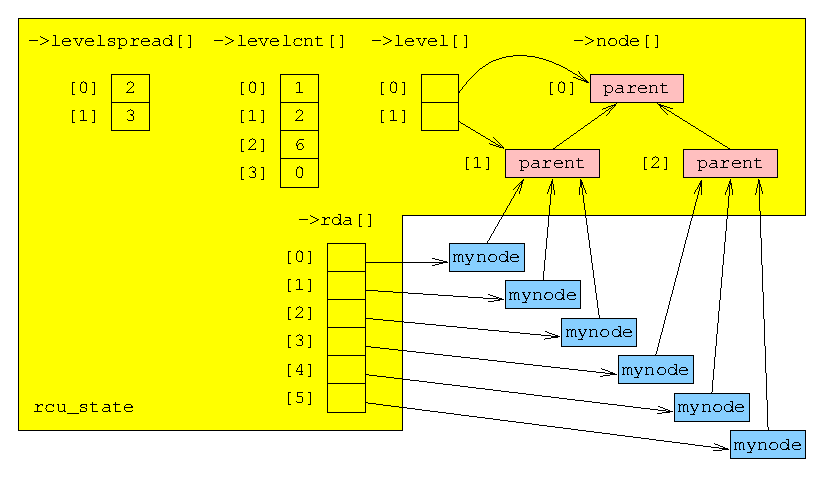
\includegraphics{appendix/rcuimpl/RCUTreeInit}}
\end{center}
\caption{Initialized RCU Data Layout}
\label{fig:app:rcuimpl:rcutree:Initialized RCU Data Layout}
\end{figure*}

This section walks through the initialization code, which links the
main data structures together as shown in
Figure~\ref{fig:app:rcuimpl:rcutree:Initialized RCU Data Layout}.
The yellow region represents fields in the \url{rcu_state} data
structure, including the \url{->node} array, individual elements
of which are shown in pink, matching the convention used in
Section~\ref{app:rcuimpl:rcutree:Hierarchical RCU Overview}.
The blue boxes each represent one \url{rcu_data} structure,
and the group of blue boxes makes up a set of per-CPU \url{rcu_data}
structures.

The \url{->levelcnt[]} array is initialized at compile time, as is
\url{->level[0]}, but the rest of the values and pointers are filled
in by the functions described in the following sections.
The figure shows a two-level hierarchy, but one-level and three-level
hierarchies are possible as well.
Each element of the \url{->levelspread[]} array gives the number of
children per node at the corresponding level of the hierarchy.
In the figure, therefore, the root node has two children and the
nodes at the leaf level each have three children.
Each element of the \url{levelcnt[]} array indicates how many nodes
there are on the corresponding level of the hierarchy: 1 at the root
level, 2 at the leaf level, and 6 at the \url{rcu_data} level---and any
extra elements are unused and left as zero.
Each element of the \url{->level[]} array references the first
node of the corresponding level of the \url{rcu_node} hierarchy,
and each element of the \url{->rda[]} array references the corresponding
CPU's \url{rcu_data} structure.
Finally, the \url{->mynode} field of each \url{rcu_data} structure
references its parent \url{rcu_node} structure.

Again, the following sections walk through the code that builds this
structure.

\subsubsection{\tt rcu\_init\_levelspread()}
\label{app:rcuimpl:rcutreewt:rcu-init-levelspread}

\begin{figure}[tbp]
{ \scriptsize
\begin{verbatim}
  1 #ifdef CONFIG_RCU_FANOUT_EXACT
  2 static void __init
  3 rcu_init_levelspread(struct rcu_state *rsp)
  4 {
  5   int i;
  6 
  7   for (i = NUM_RCU_LVLS - 1; i >= 0; i--)
  8     rsp->levelspread[i] = CONFIG_RCU_FANOUT;
  9 }
 10 #else
 11 static void __init
 12 rcu_init_levelspread(struct rcu_state *rsp)
 13 {
 14   int ccur;
 15   int cprv;
 16   int i;
 17 
 18   cprv = NR_CPUS;
 19   for (i = NUM_RCU_LVLS - 1; i >= 0; i--) {
 20     ccur = rsp->levelcnt[i];
 21     rsp->levelspread[i] = (cprv + ccur - 1) / ccur;
 22     cprv = ccur;
 23   }
 24 }
 25 #endif
\end{verbatim}
}
\caption{{\tt rcu\_init\_levelspread()} Code}
\label{fig:app:rcuimpl:rcutreewt:Code for rcu-init-levelspread}
\end{figure}

Figure~\ref{fig:app:rcuimpl:rcutreewt:Code for rcu-init-levelspread}
shows the code for the \url{rcu_init_levelspread()} function, which controls
the fanout, or the number of children per parent,
in the \url{rcu_node} hierarchy.
There are two versions of this function, one shown on lines~2-9 that
enforces the exact fanout (specified by \url{CONFIG_RCU_FANOUT}),
and the other on lines~11-25 that determines the number of child nodes
based indirectly on the specified fanout, but then balances the tree.
The \url{CONFIG_RCU_FANOUT_EXACT} kernel parameter selects which version
to use for a given kernel build.

The exact-fanout version simply assigns all of the elements of the
specified \url{rcu_state} structure's \url{->levelspread} array to
the \url{CONFIG_RCU_FANOUT} kernel parameter, as shown by the loop
on lines~7 and 8.

The hierarchy-balancing version on lines~11-24
uses a pair of local variables \url{ccur} and \url{cprv} which track
the number of \url{rcu_node} structures on the current and previous
levels, respectively.
This function works from the leaf level up the hierarchy, so \url{cprv}
is initialized by line~18 to \url{NR_CPUS}, which corresponds
to the number of \url{rcu_data} structures that feed into the leaf level.
Lines~19-23 iterate from the leaf to the root.
Within this loop, line~20 picking up
the number of \url{rcu_node} structures for the current level into
\url{ccur}.
Line~21 then rounds up the ratio of the number of nodes on the previous
(lower) level (be they \url{rcu_node} or \url{rcu_data})
to the number of \url{rcu_node} structures on the current
level, placing the result in the specified \url{rcu_state} structure's
\url{->levelspread} array.
Line~22 then sets up for the next pass through the loop.

After a call to either function, the \url{->levelspread} array contains
the number of children for each level of the \url{rcu_node} hierarchy.

\subsubsection{\tt rcu\_init\_one()}
\label{app:rcuimpl:rcutreewt:rcu-init-one}

\begin{figure}[tbp]
{ \scriptsize
\begin{verbatim}
  1 static void __init rcu_init_one(struct rcu_state *rsp)
  2 {
  3   int cpustride = 1;
  4   int i;
  5   int j;
  6   struct rcu_node *rnp;
  7 
  8   for (i = 1; i < NUM_RCU_LVLS; i++)
  9     rsp->level[i] = rsp->level[i - 1] +
 10                     rsp->levelcnt[i - 1];
 11   rcu_init_levelspread(rsp);
 12   for (i = NUM_RCU_LVLS - 1; i >= 0; i--) {
 13     cpustride *= rsp->levelspread[i];
 14     rnp = rsp->level[i];
 15     for (j = 0; j < rsp->levelcnt[i]; j++, rnp++) {
 16       spin_lock_init(&rnp->lock);
 17       rnp->qsmask = 0;
 18       rnp->qsmaskinit = 0;
 19       rnp->grplo = j * cpustride;
 20       rnp->grphi = (j + 1) * cpustride - 1;
 21       if (rnp->grphi >= NR_CPUS)
 22         rnp->grphi = NR_CPUS - 1;
 23       if (i == 0) {
 24         rnp->grpnum = 0;
 25         rnp->grpmask = 0;
 26         rnp->parent = NULL;
 27       } else {
 28         rnp->grpnum = j % rsp->levelspread[i - 1];
 29         rnp->grpmask = 1UL << rnp->grpnum;
 30         rnp->parent = rsp->level[i - 1] +
 31                 j / rsp->levelspread[i - 1];
 32       }
 33       rnp->level = i;
 34     }
 35   }
 36 }
\end{verbatim}
}
\caption{{\tt rcu\_init\_one()} Code}
\label{fig:app:rcuimpl:rcutreewt:Code for rcu-init-one}
\end{figure}

Figure~\ref{fig:app:rcuimpl:rcutreewt:Code for rcu-init-one}
shows the code for \url{rcu_init_one()}, which does boot-time initialization
for the specified 
\url{rcu_state} structure.

Recall from
Section~\ref{app:rcuimpl:rcutreewt:RCU Global State}
that the \url{->levelcnt[]} array in the \url{rcu_state} structure
is compile-time initialized to the number of nodes at each level of
the hierarchy starting from the root,
with an additional element in the array initialized
to the maximum possible number of CPUs, \url{NR_CPUS}.
In addition, the first element of the \url{->level[]} array is compile-time
initialized to reference to the root \url{rcu_node} structure, which is
in turn
the first element of the \url{->node[]} array in the \url{rcu_state} structure.
This array is further laid out in breadth-first order.
Keeping all of this in mind, the loop at lines~8-10 initializes the rest
of the \url{->level[]} array to reference the first \url{rcu_node} structure
of each level of the \url{rcu_node} hierarchy.

Line~11 then invokes \url{rcu_init_levelspread()}, which fills in the
\url{->levelspread[]} array, as was described in
Section~\ref{app:rcuimpl:rcutreewt:rcu-init-levelspread}.
The auxiliary arrays are then fully initialized, and thus ready for
the loop from lines~15-35, each pass through which initializes
one level of the \url{rcu_node} hierarchy, starting from the leaves.

Line~13 computes the number of CPUs per \url{rcu_node} structure for
the current level of the hierarchy, and line~14 obtains a pointer
to the first \url{rcu_node} structure on the current level of the
hierarchy, in preparation for the loop from lines~15-34, each pass
through which initializes one \url{rcu_node} structure.

Lines~16-18 initialize the \url{rcu_node} structure's spinlock and
its CPU masks.
The \url{qsmaskinit} field will have bits set as CPUs come online
later in boot, and the \url{qsmask} field will have bits set
when the first grace period starts.
Line~19 sets the \url{->grplo} field to the number of the this
\url{rcu_node} structure's first CPU and line~20 sets the
\url{->grphi} to the number of this \url{rcu_node} structure's
last CPU.
If the last \url{rcu_node} structure on a given level of the
hierarchy is only partially full, lines~21 and 22 set its
\url{->grphi} field to the number of the last possible CPU in the system.

Lines~24-26 initialize the \url{->grpnum}, \url{->grpmask}, and
\url{->parent} fields for the root \url{rcu_node} structure, which
has no parent, hence the zeroes and NULL.
Lines~28-31 initialize these same fields for the rest of the
\url{rcu_node} structures in the hierarchy.
Line~28 computes the \url{->grpnum} field as the index of this
\url{rcu_node} structure within
the set having the same parent, and 
line~29 sets the corresponding bit in the \url{->grpmask} field.
Finally, lines~30-31 places a pointer to the parent node into the
\url{->parent} field.
These three fields will used to propagate quiescent states up the
hierarchy.

Finally, line~33 records the hierarchy level in \url{->level},
which is used for tracing when traversing the full hierarchy.

\subsubsection{\tt \_\_rcu\_init()}
\label{app:rcuimpl:rcutreewt:rcu-init}

\begin{figure}[tbp]
{ \scriptsize
\begin{verbatim}
  1 #define RCU_DATA_PTR_INIT(rsp, rcu_data) \
  2 do { \
  3   rnp = (rsp)->level[NUM_RCU_LVLS - 1]; \
  4   j = 0; \
  5   for_each_possible_cpu(i) { \
  6     if (i > rnp[j].grphi) \
  7       j++; \
  8     per_cpu(rcu_data, i).mynode = &rnp[j]; \
  9     (rsp)->rda[i] = &per_cpu(rcu_data, i); \
 10   } \
 11 } while (0)
 12 
 13 void __init __rcu_init(void)
 14 {
 15   int i;
 16   int j;
 17   struct rcu_node *rnp;
 18 
 19   rcu_init_one(&rcu_state);
 20   RCU_DATA_PTR_INIT(&rcu_state, rcu_data);
 21   rcu_init_one(&rcu_bh_state);
 22   RCU_DATA_PTR_INIT(&rcu_bh_state, rcu_bh_data);
 23 
 24   for_each_online_cpu(i)
 25     rcu_cpu_notify(&rcu_nb, CPU_UP_PREPARE,
 26                    (void *)(long)i);
 27   register_cpu_notifier(&rcu_nb);
 28 }
\end{verbatim}
}
\caption{{\tt \_\_rcu\_init()} Code}
\label{fig:app:rcuimpl:rcutreewt:Code for rcu-init}
\end{figure}

Figure~\ref{fig:app:rcuimpl:rcutreewt:Code for rcu-init}
shows the \url{__rcu_init()} function and its \url{RCU_DATA_PTR_INIT()}
helper macro.
The \url{__rcu_init()} function is invoked during early boot,
before the scheduler has initialized, and before more than one
CPU is running.

The \url{RCU_DATA_PTR_INIT()} macro takes as arguments a pointer to
an \url{rcu_state} structure and the name of a set of \url{rcu_data}
per-CPU variables.
This macro scans the per-CPU \url{rcu_data}
structures, assigning the \url{->mynode} pointer of each \url{rcu_data}
structure to point to the corresponding leaf \url{rcu_node} structure.
It also fills out the specified \url{rcu_state} structure's
\url{->rda[]} array entries to each point to the corresponding
\url{rcu_data} structure.
Line~3 picks up a pointer to the first leaf \url{rcu_node} structure
in local variable \url{rnp} (which must be declared by the invoker of
this macro),
and line~4 sets local variable \url{j} to the corresponding leaf-node
number of zero.
Each pass through the loop spanning lines~5-10 performs initialization
for the corresponding potential CPU (as specified by \url{NR_CPUS}).
Within this loop, line~6 checks to see if we have moved beyond the
bounds of the current leaf \url{rcu_node} structure, and, if so,
line~7 advances to the next structure.
Then, still within the loop, line~8 sets the \url{->mynode} pointer
of the current CPU's \url{rcu_data} structure to reference the current
leaf \url{rcu_node} structure, and line~9 sets the current CPU's \url{->rda[]}
element (within the \url{rcu_state} structure) to reference the
current CPU's \url{rcu_data} structure.

\QuickQuiz{C-preprocessor macros are \emph{so} 1990s!
	Why not get with the times and convert \url{RCU_DATA_PTR_INIT()}
	in Figure~\ref{fig:app:rcuimpl:rcutreewt:Code for rcu-init}
	to be a function?}
\QuickQuizAnswer{
	Because, although it is possible to pass a reference to
	a particular CPU's instance of a per-CPU variable to a function,
	there does not appear to be a good way pass a reference to
	the full set of instances of a given per-CPU variable to
	a function.
	One could of course build an array of pointers, then pass a
	reference to the array in, but that is part of what
	the \url{RCU_DATA_PTR_INIT()} macro is doing in the first place.
} \QuickQuizEnd

The \url{__rcu_init()} function first invokes \url{rcu_init_one()}
on the \url{rcu_state} structure on line~19, then invokes
\url{RCU_DATA_PTR_INIT()} on the \url{rcu_state} structure and
the \url{rcu_data} set of per-CPU variables.
It then repeats this for \url{rcu_bh_state} and \url{rcu_bh_data}
on lines~21-22.
The loop spanning lines~24-26 invokes \url{rcu_cpu_notify()} for
each CPU that is currently online (which should be only the boot
CPU), and line~27 registers a notifier so that \url{rcu_cpu_notify()}
will be invoked each time a CPU comes online, in order to inform
RCU of its presence.

\QuickQuiz{What happens if a CPU comes online between the time
	that the last online CPU is notified on lines~25-26 of
	Figure~\ref{fig:app:rcuimpl:rcutreewt:Code for rcu-init}
	and the time that \url{register_cpu_notifier()} is invoked
	on line~27?}
\QuickQuizAnswer{
	Only one CPU is online at this point, so the only way another
	CPU can come online is if this CPU puts it online, which it
	is not doing.
} \QuickQuizEnd

The \url{rcu_cpu_notify()} and related functions are discussed in
Section~\ref{app:rcuimpl:rcutreewt:CPU Hotplug}
below.

\subsection{CPU Hotplug}
\label{app:rcuimpl:rcutreewt:CPU Hotplug}

The CPU-hotplug functions described in the following sections
allow RCU to track which CPUs are and are not present, but also
complete initialization of each CPU's \url{rcu_data} structure
as that CPU comes online.

\subsubsection{\tt rcu\_init\_percpu\_data()}
\label{app:rcuimpl:rcutreewt:rcu-init-percpu-data}

\begin{figure}[tbp]
{ \scriptsize
\begin{verbatim}
  1 static void
  2 rcu_init_percpu_data(int cpu, struct rcu_state *rsp)
  3 {
  4   unsigned long flags;
  5   int i;
  6   long lastcomp;
  7   unsigned long mask;
  8   struct rcu_data *rdp = rsp->rda[cpu];
  9   struct rcu_node *rnp = rcu_get_root(rsp);
 10 
 11   spin_lock_irqsave(&rnp->lock, flags);
 12   lastcomp = rsp->completed;
 13   rdp->completed = lastcomp;
 14   rdp->gpnum = lastcomp;
 15   rdp->passed_quiesc = 0;
 16   rdp->qs_pending = 1;
 17   rdp->beenonline = 1;
 18   rdp->passed_quiesc_completed = lastcomp - 1;
 19   rdp->grpmask = 1UL << (cpu - rdp->mynode->grplo);
 20   rdp->nxtlist = NULL;
 21   for (i = 0; i < RCU_NEXT_SIZE; i++)
 22     rdp->nxttail[i] = &rdp->nxtlist;
 23   rdp->qlen = 0;
 24   rdp->blimit = blimit;
 25 #ifdef CONFIG_NO_HZ
 26   rdp->dynticks = &per_cpu(rcu_dynticks, cpu);
 27 #endif /* #ifdef CONFIG_NO_HZ */
 28   rdp->cpu = cpu;
 29   spin_unlock(&rnp->lock);
 30   spin_lock(&rsp->onofflock);
 31   rnp = rdp->mynode;
 32   mask = rdp->grpmask;
 33   do {
 34     spin_lock(&rnp->lock);
 35     rnp->qsmaskinit |= mask;
 36     mask = rnp->grpmask;
 37     spin_unlock(&rnp->lock);
 38     rnp = rnp->parent;
 39   } while (rnp != NULL && !(rnp->qsmaskinit & mask));
 40   spin_unlock(&rsp->onofflock);
 41   cpu_quiet(cpu, rsp, rdp, lastcomp);
 42   local_irq_restore(flags);
 43 }
\end{verbatim}
}
\caption{{\tt rcu\_init\_percpu\_data()} Code}
\label{fig:app:rcuimpl:rcutreewt:Code for rcu-init-percpu-data}
\end{figure}

Figure~\ref{fig:app:rcuimpl:rcutreewt:Code for rcu-init-percpu-data}
shows the code for \url{rcu_init_percpu_data()}, which initializes
the specified CPU's \url{rcu_data} structure in response to booting
up or to that CPU coming online.
It also sets up the \url{rcu_node} hierarchy so that this CPU will
participate in future grace periods.

Line~8 gets a pointer to this CPU's \url{rcu_data} structure, based
on the specified \url{rcu_state} structure, and places this pointer
into the local variable \url{rdp}.
Line~9 gets a pointer to the root \url{rcu_node} structure for the
specified \url{rcu_state} structure, placing it in local variable
\url{rnp}.

Lines~11-29 initialize the fields of the \url{rcu_data} structure
under the protection of the root \url{rcu_node} structure's lock
in order to ensure consistent values.
Line~17 is important for tracing, due to the fact that many Linux
distributions set \url{NR_CPUS} to a very large number, which could
result in excessive output when tracing \url{rcu_data} structures.
The \url{->beenonline} field is used to solve this problem, as
it will be set to the value one on any \url{rcu_data} structure
corresponding to a CPU that has ever been online, and set to zero
for all other \url{rcu_data} structures.
This allows the tracing code to easily ignore irrelevant CPUs.

Lines~30-40 propagate the onlining CPU's bit up the \url{rcu_node}
hierarchy, proceeding until either the root \url{rcu_node} is
reached or until the corresponding bit is already set, whichever
comes first.
This bit-setting is done under the protection of \url{->onofflock}
in order to exclude initialization of a new grace period, and, in addition,
each \url{rcu_node} structure is initialized under the protection
of its lock.
Line~41 then invokes \url{cpu_quiet()} to signal RCU that this
CPU has been in an extended quiescent state, and finally, line~42
re-enables irqs.

\QuickQuiz{Why call \url{cpu_quiet()} on line~41 of
	Figure~\ref{fig:app:rcuimpl:rcutreewt:Code for rcu-init-percpu-data},
	given that we are excluding grace periods with various
	locks, and given that any earlier grace periods would not have
	been waiting on this previously-offlined CPU?}
\QuickQuizAnswer{
	A new grace period might have started just after the
	\url{->onofflock} was released on line~40.
	The \url{cpu_quiet()} will help expedite such a grace period.
} \QuickQuizEnd

It is important to note that \url{rcu_init_percpu_data()} is invoked
not only at boot time, but also every time that a given CPU is brought
online.

\subsubsection{\tt rcu\_online\_cpu()}
\label{app:rcuimpl:rcutreewt:rcu-online-cpu}

\begin{figure}[tbp]
{ \scriptsize
\begin{verbatim}
  1 static void __cpuinit rcu_online_cpu(int cpu)
  2 {
  3 #ifdef CONFIG_NO_HZ
  4   struct rcu_dynticks *rdtp;
  5 
  6   rdtp = &per_cpu(rcu_dynticks, cpu);
  7   rdtp->dynticks_nesting = 1;
  8   rdtp->dynticks |= 1;
  9   rdtp->dynticks_nmi = (rdtp->dynticks_nmi + 1) & ~0x1;
 10 #endif /* #ifdef CONFIG_NO_HZ */
 11   rcu_init_percpu_data(cpu, &rcu_state);
 12   rcu_init_percpu_data(cpu, &rcu_bh_state);
 13   open_softirq(RCU_SOFTIRQ, rcu_process_callbacks);
 14 }
\end{verbatim}
}
\caption{{\tt rcu\_online\_cpu()} Code}
\label{fig:app:rcuimpl:rcutreewt:Code for rcu-online-cpu}
\end{figure}

Figure~\ref{fig:app:rcuimpl:rcutreewt:Code for rcu-online-cpu}
shows the code for \url{rcu_online_cpu()}, which informs RCU that the
specified CPU is coming online.

When dynticks (\url{CONFIG_NO_HZ}) is enabled, line~6 obtains a
reference to the specified CPU's \url{rcu_dynticks} structure, which
is shared between the ``rcu'' and ``rcu\_bh'' implementations of RCU.
Line~7 sets the \url{->dynticks_nesting} field to the value one,
reflecting the fact that a newly onlined CPU is not in dynticks-idle
mode (recall that the \url{->dynticks_nesting} field tracks the
number of reasons that the corresponding CPU needs to be tracked for
RCU read-side critical sections, in this case because it can run
process-level code).
Line~8 forces the \url{->dynticks} field to an odd value that is
at least as large as the last value it had when previously online,
again reflecting the fact that newly onlined CPUs are not in dynticks-idle
mode, and line~9 forces the \url{->dynticks_nmi} field to an even value
that is at least as large as the last value it had when previously
online, reflecting the fact that this CPU is not currently executing
in an NMI handler.

Lines~11-13 are executed regardless of the value of the
\url{CONFIG_NO_HZ} kernel parameter.
Line~11 initializes the specified CPU's \url{rcu_data} structure
for ``rcu'', and line~12 does so for ``rcu\_bh''.
Finally, line~13 registers the \url{rcu_process_callbacks()} to be
invoked by subsequent \url{raise_softirq()} invocations on this CPU.

\subsubsection{\tt rcu\_offline\_cpu()}
\label{app:rcuimpl:rcutreewt:rcu-offline-cpu}

\begin{figure}[tbp]
{ \scriptsize
\begin{verbatim}
  1 static void
  2 __rcu_offline_cpu(int cpu, struct rcu_state *rsp)
  3 {
  4   int i;
  5   unsigned long flags;
  6   long lastcomp;
  7   unsigned long mask;
  8   struct rcu_data *rdp = rsp->rda[cpu];
  9   struct rcu_data *rdp_me;
 10   struct rcu_node *rnp;
 11 
 12   spin_lock_irqsave(&rsp->onofflock, flags);
 13   rnp = rdp->mynode;
 14   mask = rdp->grpmask;
 15   do {
 16     spin_lock(&rnp->lock);
 17     rnp->qsmaskinit &= ~mask;
 18     if (rnp->qsmaskinit != 0) {
 19       spin_unlock(&rnp->lock);
 20       break;
 21     }
 22     mask = rnp->grpmask;
 23     spin_unlock(&rnp->lock);
 24     rnp = rnp->parent;
 25   } while (rnp != NULL);
 26   lastcomp = rsp->completed;
 27   spin_unlock(&rsp->onofflock);
 28   cpu_quiet(cpu, rsp, rdp, lastcomp);
 29   rdp_me = rsp->rda[smp_processor_id()];
 30   if (rdp->nxtlist != NULL) {
 31     *rdp_me->nxttail[RCU_NEXT_TAIL] = rdp->nxtlist;
 32     rdp_me->nxttail[RCU_NEXT_TAIL] =
 33         rdp->nxttail[RCU_NEXT_TAIL];
 34     rdp->nxtlist = NULL;
 35     for (i = 0; i < RCU_NEXT_SIZE; i++)
 36       rdp->nxttail[i] = &rdp->nxtlist;
 37     rdp_me->qlen += rdp->qlen;
 38     rdp->qlen = 0;
 39   }
 40   local_irq_restore(flags);
 41 }
 42 
 43 static void rcu_offline_cpu(int cpu)
 44 {
 45   __rcu_offline_cpu(cpu, &rcu_state);
 46   __rcu_offline_cpu(cpu, &rcu_bh_state);
 47 }
\end{verbatim}
}
\caption{{\tt rcu\_offline\_cpu()} Code}
\label{fig:app:rcuimpl:rcutreewt:Code for rcu-offline-cpu}
\end{figure}

Figure~\ref{fig:app:rcuimpl:rcutreewt:Code for rcu-offline-cpu}
shows the code for \url{__rcu_offline_cpu()} and its wrapper
function, \url{rcu_offline_cpu()}.
The purpose of this wrapper function (shown in lines~43-47 of the figure)
is simply to invoke \url{__rcu_offline_cpu()} twice, once for ``rcu'' and
again for ``rcu\_bh''.
The purpose of the \url{__rcu_offline_cpu()} function is to
prevent future grace periods from waiting on the CPU being offlined,
to note the extended quiescent state, and to find a new home for
any RCU callbacks in process on this CPU.

Turning to \url{__rcu_offline_cpu()}, shown on lines~1-41 of the figure,
line~12 acquires the specified \url{rcu_state} structure's
\url{->onofflock}, excluding grace-period initialization for
multi-\url{rcu_node} hierarchies.

\QuickQuiz{But what if the \url{rcu_node} hierarchy has only a single
	structure, as it would on a small system?
	What prevents concurrent grace-period initialization in that
	case, given the code in
	Figure~\ref{fig:app:rcuimpl:rcutreewt:Code for rcu-offline-cpu}?}
\QuickQuizAnswer{
	The later acquisition of the sole \url{rcu_node} structure's
	\url{->lock} on line~16 excludes grace-period initialization,
	which must acquire this same lock in order to initialize this
	sole \url{rcu_node} structure for the new grace period.

	The \url{->onofflock} is needed only for multi-node hierarchies,
	and is used in that case as an alternative to acquiring and
	holding \emph{all} of the \url{rcu_node} structures'
	\url{->lock} fields, which would be incredibly painful on
	large systems.
} \QuickQuizEnd

Line~13 picks up a pointer to the leaf \url{rcu_node} structure corresponding
to this CPU, using the \url{->mynode} pointer in this CPU's \url{rcu_data}
structure
(see Figure~\ref{fig:app:rcuimpl:rcutree:Initialized RCU Data Layout}).
Line~14 picks up a mask with this CPU's bit set for use on
the leaf \url{rcu_node} structure's \url{qsmask} field.

The loop spanning lines~15-25 then clears this CPU's bits up the
\url{rcu_node} hierarchy, starting with this CPU's leaf \url{rcu_node}
structure.
Line~16 acquires the current \url{rcu_node} structure's \url{->lock}
field, and line~17 clears the bit corresponding to this CPU
(or group, higher up in the hierarchy) from the \url{->qsmaskinit}
field, so that future grace periods will not wait on quiescent states
from this CPU.
If the resulting \url{->qsmaskinit} value is non-zero, as checked by
line~18, then the
current \url{rcu_node} structure has other online CPUs that it
must track, so line~19 releases the current \url{rcu_node} structure's
\url{->lock} and line~20 exits the loop.
Otherwise, we need to continue walking up the \url{rcu_node} hierarchy.
In this case, line~22 picks up the mask to apply to the next level up,
line~23 releases the current \url{rcu_node} structure's \url{->lock},
and line~24 advances up to the next level of the hierarchy.
Line~25 exits the loop should we exit out the top of the hierarchy.

\QuickQuiz{But does line~25 of
	Figure~\ref{fig:app:rcuimpl:rcutreewt:Code for rcu-offline-cpu}
	ever really exit the loop?
	Why or why not?}
\QuickQuizAnswer{
	The only way that line~25 could exit the loop is if \emph{all}
	CPUs were to be put offline.
	This cannot happen in the Linux kernel as of 2.6.28, though
	other environments have been designed to offline all CPUs
	during the normal shutdown procedure.
} \QuickQuizEnd

Line~26 picks up the the specified \url{rcu_state} structure's
\url{->completed} field into the local variable \url{lastcomp},
line~27 releases \url{->onofflock} (but leaves irqs disabled),
and line~28 invokes \url{cpu_quiet()} in order to note that the
CPU being offlined is now in an extended quiescent state, passing
in \url{lastcomp} to avoid reporting this quiescent state against
a different grace period than it occurred in.

\QuickQuiz{Suppose that line~26 got executed seriously out of order in
	Figure~\ref{fig:app:rcuimpl:rcutreewt:Code for rcu-offline-cpu},
	so that \url{lastcomp} is set to some prior grace period, but
	so that the current grace period is still waiting on the
	now-offline CPU?
	In this case, won't the call to \url{cpu_quiet()} fail to
	report the quiescent state, thus causing the grace period
	to wait forever for this now-offline CPU?}
\QuickQuizAnswer{
	First, the lock acquisitions on lines~16 and 12 would prevent
	the execution of line~26 from being pushed that far out of
	order.
	Nevertheless, even if line~26 managed to be misordered that
	dramatically, what would happen is that \url{force_quiescent_state()}
	would eventually be invoked, and would notice that the current
	grace period was waiting for a quiescent state from an offline
	CPU.
	Then \url{force_quiescent_state()} would report the extended
	quiescent state on behalf of the offlined CPU.
} \QuickQuizEnd

\QuickQuiz{Given that an offline CPU is in an extended quiescent state,
	why does line~28 of
	Figure~\ref{fig:app:rcuimpl:rcutreewt:Code for rcu-offline-cpu}
	need to care which grace period it is
	dealing with?}
\QuickQuizAnswer{
	It really does not need to care in this case.
	However, because it \emph{does} need to care in many other
	cases, the \url{cpu_quiet()} function does take the
	grace-period number as an argument, so some value must be
	supplied.
} \QuickQuizEnd

Lines~29-39 move any RCU callbacks from the CPU going offline to the
currently running CPU.
This operation must avoid reordering the callbacks being moved, as
otherwise \url{rcu_barrier()} will not work correctly.
Line~29 puts a pointer to the currently running CPU's \url{rcu_data}
structure into local variable \url{rdp_me}.
Line~30 then checks to see if the CPU going offline has any RCU callbacks.
If so, lines~31-38 move them.
Line~31 splices the list of callbacks onto the end of the running CPU's
list.
Lines~32-33 sets the running CPU's callback tail pointer to that of
the CPU going offline, and then lines 34-36 initialize the going-offline
CPU's list to be empty.
Line~37 adds the length of the going-offline CPU's callback list to
that of the currently running CPU, and, finally, line 38 zeroes the
going-offline CPU's list length.

\QuickQuiz{But this list movement in 
	Figure~\ref{fig:app:rcuimpl:rcutreewt:Code for rcu-offline-cpu}
	makes all of the going-offline CPU's callbacks go through
	another grace period, even if they were ready to invoke.
	Isn't that inefficient?
	Furthermore, couldn't an unfortunate pattern of CPUs going
	offline then coming back online prevent a given callback from
	ever being invoked?}
\QuickQuizAnswer{
	It is inefficient, but it is simple.
	Given that this is not a commonly executed code path, this
	is the right tradeoff.
	The starvation case would be a concern, except that the
	online and offline process involves multiple grace periods.
} \QuickQuizEnd

Finally, line~40 re-enables irqs.

@@@

% initialization, online/offline
% __rcu_offline_cpu, rcu_offline_cpu (empty if !CONFIG_HOTPLUG_CPU)
%DONE% \url{__rcu_init()}.
%DONE%	rcu_online_cpu,
%DONE%	rcu_init_percpu_data
%DONE%	rcu_init_levelspread (CONFIG_RCU_FANOUT_EXACT and not)
%DONE%	rcu_init_one, 

\subsection{Forcing Quiescent States}
\label{app:rcuimpl:rcutreewt:Forcing Quiescent States}

Normally, CPUs pass through quiescent states which are duly recorded,
so that grace periods end in a timely manner.
However, any of the following three conditions can prevent CPUs from
passing through quiescent states:

\begin{enumerate}
\item	The CPU is in dyntick-idle state, and is sleeping in a low-power
	mode.
	Although such a CPU is officially in an extended quiescent state,
	because it is not executing instructions, it cannot do anything
	on its own.
\item	The CPU is in the process of coming online, and RCU has been
	informed that it is online, but this CPU is not yet actually
	executing code, nor is it marked as online in \url{cpu_online_map}.
	The current grace period will therefore wait on it, but it cannot
	yet pass through quiescent states on its own.
\item	The CPU is running user-level code, but has avoided
	entering the scheduler for an extended time period.
\end{enumerate}

In each of these cases, RCU needs to take action on behalf of the
non-responding CPU.
This section describes the functions that take such action.

% rcu_process_dyntick

% @@@ the code in the following figure needs to be redone: recently changed.

\begin{figure}[tbp]
{ \scriptsize
\begin{verbatim}
  1 static void
  2 force_quiescent_state(struct rcu_state *rsp, int relaxed)
  3 {
  4   unsigned long flags;
  5   long lastcomp;
  6   struct rcu_data *rdp = rsp->rda[smp_processor_id()];
  7   struct rcu_node *rnp = rcu_get_root(rsp);
  8   u8 signaled;
  9 
 10   if (ACCESS_ONCE(rsp->completed) ==
 11       ACCESS_ONCE(rsp->gpnum))
 12     return;
 13   if (!spin_trylock_irqsave(&rsp->fqslock, flags)) {
 14     rsp->n_force_qs_lh++;
 15     return;
 16   }
 17   if (relaxed &&
 18       (long)(rsp->jiffies_force_qs - jiffies) >= 0 &&
 19       (rdp->n_rcu_pending_force_qs -
 20        rdp->n_rcu_pending) >= 0)
 21     goto unlock_ret;
 22   rsp->n_force_qs++;
 23   spin_lock(&rnp->lock);
 24   lastcomp = rsp->completed;
 25   signaled = rsp->signaled;
 26   rsp->jiffies_force_qs =
 27     jiffies + RCU_JIFFIES_TILL_FORCE_QS;
 28   rdp->n_rcu_pending_force_qs =
 29     rdp->n_rcu_pending +
 30     RCU_JIFFIES_TILL_FORCE_QS;
 31   if (lastcomp == rsp->gpnum) {
 32     rsp->n_force_qs_ngp++;
 33     spin_unlock(&rnp->lock);
 34     goto unlock_ret;
 35   }
 36   spin_unlock(&rnp->lock);
 37   switch (signaled) {
 38   case RCU_GP_INIT:
 39     break;
 40   case RCU_SAVE_DYNTICK:
 41     if (RCU_SIGNAL_INIT != RCU_SAVE_DYNTICK)
 42       break;
 43     if (rcu_process_dyntick(rsp, lastcomp,
 44           dyntick_save_progress_counter))
 45       goto unlock_ret;
 46     spin_lock(&rnp->lock);
 47     if (lastcomp == rsp->completed) {
 48       rsp->signaled = RCU_FORCE_QS;
 49       dyntick_record_completed(rsp, lastcomp);
 50     }
 51     spin_unlock(&rnp->lock);
 52     break;
 53   case RCU_FORCE_QS:
 54     if (rcu_process_dyntick(rsp,
 55           dyntick_recall_completed(rsp),
 56           rcu_implicit_dynticks_qs))
 57       goto unlock_ret;
 58     break;
 59   }
 60 unlock_ret:
 61   spin_unlock_irqrestore(&rsp->fqslock, flags);
 62 }
\end{verbatim}
}
\caption{{\tt force\_quiescent\_state()} Code}
\label{fig:app:rcuimpl:rcutreewt:Code for rcutree force-quiescent-state}
\end{figure}

Figure~\ref{fig:app:rcuimpl:rcutreewt:Code for rcutree force-quiescent-state}
shows the code for \url{force_quiescent_state()} for
\url{CONFIG_SMP},\footnote{
	For non-\url{CONFIG_SMP}, \url{force_quiescent_state} is a
	simple wrapper around \url{set_need_resched()}.}
which is invoked when RCU feels the need to expedite the current
grace period by forcing CPUs through quiescent states.
RCU feels this need when either:
\begin{enumerate}
\item	the current grace period has gone on for more than three jiffies
	(or as specified by the compile-time value of
	\url{RCU_JIFFIES_TILL_FORCE_QS}), or
\item	a CPU enqueuing an RCU callback via either \url{call_rcu()}
	or \url{call_rcu_bh()} sees more than 10,000 callbacks enqueued
	(or as specified by the boot-time parameter \url{qhimark}).
\end{enumerate}

Lines~10-12 check to see if there is a grace period in progress,
silently exiting if not.
Lines~13-16 attempt to acquire \url{->fqslock}, which prevents concurrent
attempts to expedite a grace period.
The \url{->n_force_qs_lh} counter is incremented when this lock is
already held, and is visible via the \url{fqlh=} field
in the \url{rcuhier} debugfs file when the \url{CONFIG_RCU_TRACE} kernel
parameter is enabled.
Lines~17-21 check to see if it is really necessary to expedite the
current grace period, in other words, if (1) the current CPU has 10,000
RCU callbacks waiting, or (2) at least three jiffies have passed
since either the beginning of the current grace period or since the
last attempt to expedite the current grace period, measured either
by the \url{jiffies} counter or by the number of calls to
\url{rcu_pending}.
Line~22 then counts the number of attempts to expedite grace periods.

Lines~23-36 are executed with the root \url{rcu_node} structure's lock
held in order to prevent confusion should the current grace period
happen to end just as we try to expedite it.
Lines~24 and 25 snapshot the \url{->completed} and \url{\signaled} fields,
lines~26-30 set the soonest time that a subsequent non-relaxed
\url{force_quiescent_state()} will be allowed to actually do
any expediting, and lines~31-35 check to see if the grace period
ended while we were acquiring the \url{rcu_node} structure's lock,
releasing this lock and returning if so.

Lines~37-59 drive the \url{force_quiescent_state()} state machine.
If the grace period is still in the midst of initialization,
lines~41 and 42 simply return, allowing \url{force_quiescent_state()}
to be called again at a later time, presumably after initialization
has completed.
If dynticks are enabled (via the \url{CONFIG_NO_HZ} kernel
parameter), the first post-initialization call
to \url{force_quiescent_state()} in a given grace period will
execute lines~40-52, and the second and subsequent calls will
execute lines~53-59.
On the other hand, if dynticks is not enabled, then all post-initialization
calls to \url{force_quiescent_state()} will execute lines~53-59.

The purpose of lines~40-52 is to record the current dynticks-idle state
of all CPUs that have not yet passed through a quiescent state, and
to record a quiescent state for any that are currently in dynticks-idle
state (but not currently in an irq or NMI handler).
Lines~41-42 serve to inform gcc that this branch of the switch statement
is dead code for non-\url{CONFIG_NO_HZ} kernels.
Lines 43-45 invoke \url{rcu_process_dyntick()} in order to invoke
\url{dyntick_save_progress_counter()} for each CPU that has not yet
passed through a quiescent state for the current grace period,
exiting \url{force_quiescent_state()} if the grace period ends in
the meantime (possibly due to having found that all the CPUs that
had not yet passed through a quiescent state were sleeping in
dyntick-idle mode).
Lines~46 and 51 acquire and release the root \url{rcu_node} structure's
lock, again to avoid possible confusion with a concurrent end of the
current grace period.
Line~47 checks to see if the current grace period is still in force, and,
if so, line~48 advances the state machine to the \url{RCU_FORCE_QS} state
and line~49 saves the current grace-period number for the benefit of
the next invocation of \url{force_quiescent_state()}.
The reason for saving the current grace-period number is to correctly
handle race conditions involving the current grace period ending
concurrently with the next invocation of \url{force_quiescent_state()}.

As noted earlier, lines~53-58 handle the second and subsequent invocations
of \url{force_quiescent_state()} in \url{CONFIG_NO_HZ} kernels, and \emph{all}
invocations in non-\url{CONFIG_NO_HZ} kernels.
Lines~54 and 58 invoke \url{rcu_process_dyntick()}, which cycles through
the CPUs that have still not passed through a quiescent state, invoking
\url{rcu_implicit_dynticks_qs()} on them, which in turn checks to see
if any of these CPUs have passed through dyntick-idle state (if
\url{CONFIG_NO_HZ} is enabled), checks to see if we are waiting on
any offline CPUs, and finally sends a reschedule IPI to any remaining
CPUs not in the first two groups.

@@@ read through email to gather up acknowledgments @@@

% appendix/rcuimpl/rcupreempt.tex

\section{Preemptible RCU}
\label{app:rcuimpl:Preemptible RCU}
\OriginallyPublished{Appendix}{app:rcuimpl:Preemptible RCU}{Preemptible RCU}{Linux Weekly News}{PaulEMcKenney2007PreemptibleRCU}

The preemptible RCU implementation is unusual in that
it permits read-side critical
sections to be preempted and to be blocked waiting for locks.
However, it does not handle general blocking
(for example, via the \co{wait_event()} primitive):
if you need that, you should instead use SRCU, which is described in
Appendix~\ref{app:rcuimpl:Sleepable RCU Implementation}.
In contrast to SRCU,
preemptible RCU only permits blocking within primitives that are
both subject to priority inheritance and non-blocking in a
non-\co{CONFIG_PREEMPT} kernel.
This ability to acquire blocking locks and to be preempted within
RCU read-side critical sections is required for the aggressive real-time
capabilities provided by Ingo Molnar's -rt patchset.
However, the initial preemptible RCU implementation~\cite{PaulMcKenney2005d}
had some limitations, including:

\begin{enumerate}
\item	Its read-side primitives cannot be called from within
	non-maskable interrupt (NMI) or systems-management interrupt
	handlers.
\item	Its read-side primitives use both atomic instructions and
	memory barriers, both of which have excessive overhead.
\item	It does no priority boosting of RCU read-side critical
	sections~\cite{PaulEMcKenney2007BoostRCU}.
\end{enumerate}

The new preemptible RCU implementation that accepted into the 2.6.26
Linux kernel
removes these limitations, and this appendix describes its design,
serving as an update to the LWN article~\cite{PaulEMcKenney2007PreemptibleRCU}.
However, please note that this implementation was replaced with a faster
and simpler implementation in the 2.6.32 Linux kernel.
This description nevertheless remains to bear witness to the most complex
RCU implementation ever devised.

\QuickQuiz{}
	Why is it important that blocking primitives
	called from within a preemptible-RCU read-side critical section be
	subject to priority inheritance?
\QuickQuizAnswer{
	Because blocked readers stall RCU grace periods,
	which can result in OOM.
	For example, if a reader did a \co{wait_event()} within
	an RCU read-side critical section, and that event never occurred,
	then RCU grace periods would stall indefinitely, guaranteeing that
	the system would OOM sooner or later.
	There must therefore be some way to cause these readers to progress
	through their read-side critical sections in order to avoid such OOMs.
	Priority boosting is one way to force such progress, but only if
	readers are restricted to blocking such that they can be awakened via
	priority boosting.

	Of course, there are other methods besides priority inheritance
	that handle the priority inversion problem, including priority ceiling,
	preemption disabling, and so on.
	However, there are good reasons why priority inheritance is the approach
	used in the Linux kernel, so this is what is used for RCU.
} \QuickQuizEnd

\QuickQuiz{}
	Could the prohibition against using primitives
	that would block in a non-\co{CONFIG_PREEMPT} kernel be lifted,
	and if so, under what conditions?
\QuickQuizAnswer{
	If testing and benchmarking demonstrated that the
	preemptible RCU worked well enough that classic RCU could be dispensed
	with entirely, and if priority inheritance was implemented for blocking
	synchronization primitives
	such as \co{semaphore}s, then those primitives could be
	used in RCU read-side critical sections.
} \QuickQuizEnd

\subsection{Conceptual RCU}
\label{app:rcuimpl:Conceptual RCU}

Understanding and validating an RCU implementation is much easier given
a view of RCU at the lowest possible level.
This section gives a very brief overview of the
most basic concurrency requirements that an RCU implementation must
support.
For more detail, please see
Section~\ref{sec:defer:RCU Fundamentals}.

RCU implementations must obey the following rule: if any
statement in a given RCU read-side critical section precedes a
grace period, then all statements in that RCU read-side critical
section must complete before that grace period ends.

\begin{figure}[htb]
\begin{center}
\resizebox{3in}{!}{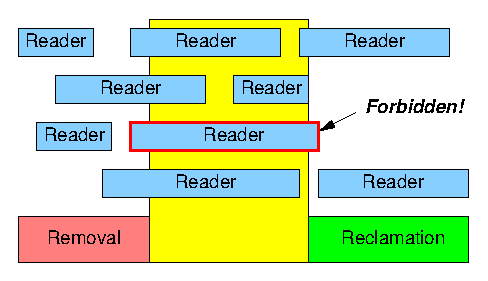
\includegraphics{appendix/rcuimpl/GracePeriodBad}}
\end{center}
\caption{Buggy Grace Period From Broken RCU}
\label{app:rcuimpl:Buggy Grace Period From Broken RCU}
\end{figure}

This is illustrated by
Figure~\ref{app:rcuimpl:Buggy Grace Period From Broken RCU},
where time advances from left to right.
The red ``Removal'' box represents the update-side critical section that
modifies the RCU-protected data structure, for example, via
\co{list_del_rcu()}; the large yellow ``Grace Period'' box
represents a grace period (surprise!) which might be invoked via
\co{synchronize_rcu()}, and the green ``Reclamation'' box
represents freeing the affected data element,
perhaps via \co{kfree()}.
The blue ``Reader'' boxes each represent an RCU read-side critical section,
for example, beginning with \co{rcu_read_lock()} and ending with
\co{rcu_read_unlock()}.
The red-rimmed ``Reader'' box is an example of an illegal situation:
any so-called RCU implementation that permits a read-side critical section
to completely overlap a grace period is buggy, since the updater might
free up memory that this reader is still using.

So, what is the poor RCU implementation to do in this situation?

\begin{figure}[htb]
\begin{center}
\resizebox{3in}{!}{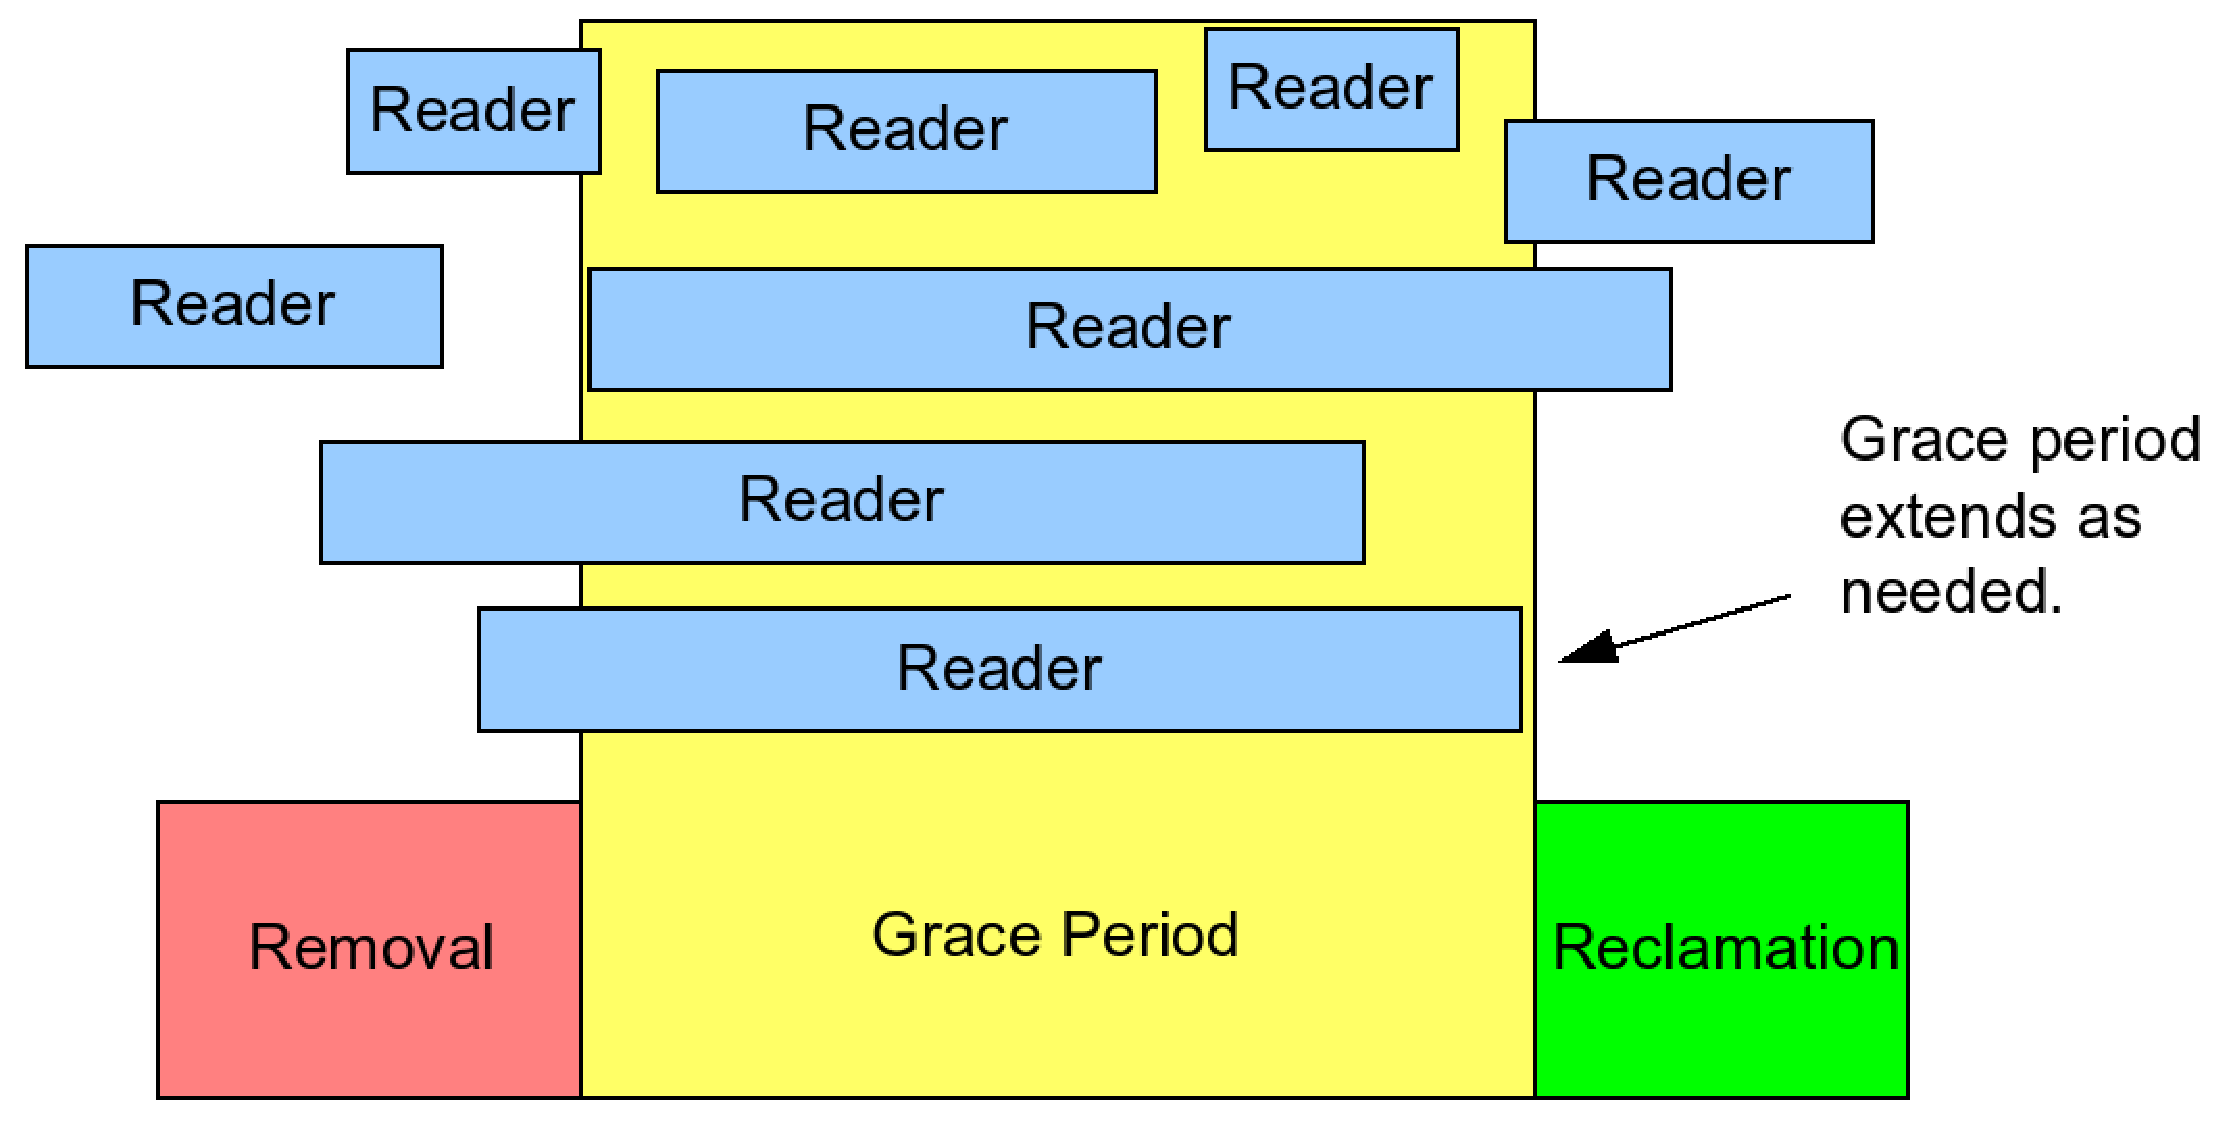
\includegraphics{appendix/rcuimpl/GracePeriodGood}}
\end{center}
\caption{Good Grace Period From Correct RCU}
\label{app:rcuimpl:Good Grace Period From Correct RCU}
\end{figure}

It must extend the grace period, perhaps as shown in
Figure~\ref{app:rcuimpl:Good Grace Period From Correct RCU}.
In short, the RCU implementation must ensure that any
RCU read-side critical sections in progress at the start of a given grace
period have completely finished, memory operations and all, before that
grace period is permitted to complete.
This fact allows RCU validation to be extremely focused: simply demonstrate
that any RCU read-side critical section in progress at the beginning of
a grace period must terminate before that grace period ends, along with
sufficient barriers to prevent either the compiler or the CPU from undoing
the RCU implementation's work.

\subsection{Overview of Preemptible RCU Algorithm}
\label{app:rcuimpl:Overview of Preemptible RCU Algorithm}

This section focuses on a specific implementation of preemptible RCU.
Many other implementations are possible, and are described
elsewhere~\cite{PaulEMcKenney2006b,PaulMcKenney05b}.
This article focuses on this specific implementation's
general approach, the data structures,
the grace-period state machine, and a walk through the read-side primitives.

\subsubsection{General Approach}
\label{app:rcuimpl:General Approach}

\begin{figure}[htb]
\begin{center}
\resizebox{3in}{!}{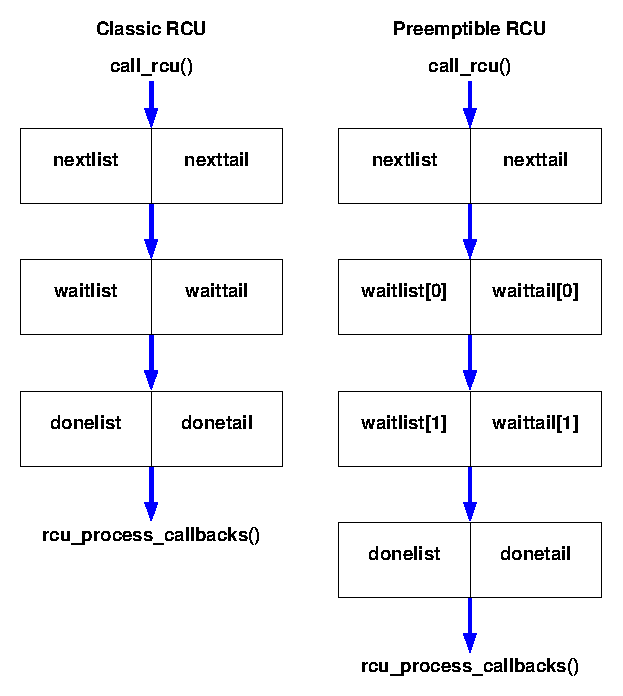
\includegraphics{appendix/rcuimpl/RCUpreemptListsCompare}}
\end{center}
\caption{Classic vs. Preemptible RCU Callback Processing}
\label{app:rcuimpl:Classic vs. Preemptible RCU Callback Processing}
\end{figure}

Because this implementation of preemptible RCU does not require memory
barriers in \co{rcu_read_lock()} and \co{rcu_read_unlock()},
a multi-stage grace-period detection algorithm is required.
Instead of using a single \co{wait} queue of callbacks
(which has sufficed for earlier RCU implementations), this implementation
uses an array of \co{wait} queues, so that RCU callbacks
are enqueued on each element of this array in turn.
This difference in callback flow is shown in
Figure~\ref{app:rcuimpl:Classic vs. Preemptible RCU Callback Processing}
for a preemptible RCU implementation with two waitlist stages per grace period
(in contrast,
the September 10 2007 patch to -rt~\cite{PaulEMcKenney2007PreemptibleRCUPatch}
uses four waitlist stages).

Given two stages per grace period, any pair of
stages forms a full grace period.
Similarly, in an implementation with four stages per grace period,
any sequence of four stages would form a full grace period.

\begin{figure}[htb]
\begin{center}
\resizebox{3in}{!}{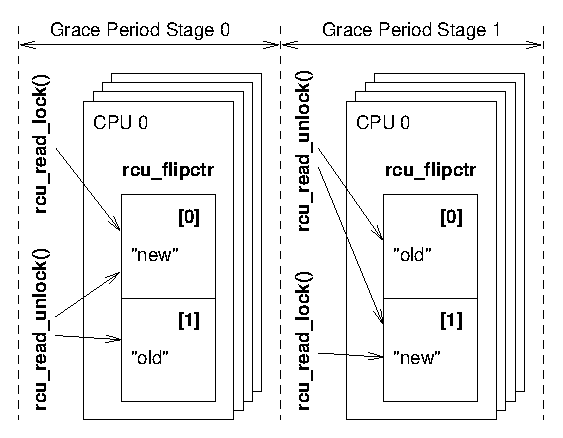
\includegraphics{appendix/rcuimpl/RCUpreemptCounterFlip}}
\end{center}
\caption{Preemptible RCU Counter Flip Operation}
\label{app:rcuimpl:Preemptible RCU Counter Flip Operation}
\end{figure}

To determine when a grace-period stage can end,
preemptible RCU uses a per-CPU two-element \co{rcu_flipctr} array
that tracks in-progress RCU read-side critical sections.
One element of a given CPU's \co{rcu_flipctr} array tracks
old RCU read-side critical sections, in other words, critical sections
that started before the current grace-period stage.
The other element tracks new RCU read-side critical
sections, namely those starting during the current grace-period stage.
The array elements switch roles at the beginning of each new grace-period
stage, as shown in
Figure~\ref{app:rcuimpl:Preemptible RCU Counter Flip Operation}.

During the first stage on the left-hand side of the above figure,
\co{rcu_flipctr[0]} tracks the new
RCU read-side critical sections, and is therefore incremented by
\co{rcu_read_lock()} and decremented by \co{rcu_read_unlock()}.
Similarly, \co{rcu_flipctr[1]} tracks the old RCU read-side
critical sections (those that started during earlier stages), and
is therefore decremented by \co{rcu_read_unlock()} and never
incremented at all.

Because each CPU's old \co{rcu_flipctr[1]} elements are never
incremented, their sum across all CPUs must eventually go to zero,
although preemption in the midst of an RCU read-side critical section might
cause any individual counter to remain non-zero or even to go negative.
For example, suppose that a task calls \co{rcu_read_lock()} on
one CPU, is preempted, resumes on another CPU, and then calls
\co{rcu_read_unlock()}.
The first CPU's counter will then be +1 and the second CPU's counter
will be -1, however, they will still sum to zero.
Regardless of possible preemption, when the sum of the old counter
elements does go to zero, it is safe to move to the next grace-period
stage, as shown on the right-hand side of the above figure.

In this second stage, the elements of each CPU's \co{rcu_flipctr}
counter array switch roles.
The \co{rcu_flipctr[0]} counter now tracks the old RCU read-side
critical sections, in other words, the ones that started during
grace period stage 0.
Similarly, the \co{rcu_flipctr[1]} counter now tracks the new
RCU read-side critical sections that start in grace period stage 1.
Therefore, \co{rcu_read_lock()} now increments
\co{rcu_flipctr[1]}, while \co{rcu_read_unlock()} still
might decrement either counter.
Specifically, if the matching \co{rcu_read_lock()} executed
during grace-period stage 0 (the old stage at this point), then
\co{rcu_read_unlock()} must decrement \co{rcu_flipctr[0]},
but if the matching \co{rcu_read_lock()} executed during
grace-period stage 1 (the new stage), then \co{rcu_read_unlock()}
must instead decrement \co{rcu_flipctr[1]}.

The critical point is that all \co{rcu_flipctr} elements
tracking the old RCU read-side critical sections must strictly decrease.
Therefore, once the sum of these old counters reaches zero,
it cannot change.

The \co{rcu_read_lock()} primitive uses the bottom
bit of the current grace-period counter
(\co{rcu_ctrlblk.completed & 0x1}) to index the
\co{rcu_flipctr} array,
and records this index in the task structure.
The matching \co{rcu_read_unlock()} uses this recorded
value to ensure that it decrements a counter corresponding to
the one that the matching \co{rcu_read_lock()} incremented.
Of course, if the RCU read-side critical section has been preempted,
\co{rcu_read_unlock()} might be decrementing the counter
belonging to a different CPU than the one whose counter was incremented
by the matching \co{rcu_read_lock()}.

Each CPU also maintains \co{rcu_flip_flag} and
\co{rcu_mb_flag} per-CPU variables.
The \co{rcu_flip_flag} variable is used to synchronize the
start of each grace-period stage: once a given CPU has responded
to its \co{rcu_flip_flag}, it must refrain from incrementing
the \co{rcu_flip} array element that now corresponds to
the old grace-period stage.
The CPU that advances the counter (\co{rcu_ctrlblk.completed})
changes the value of each CPU's \co{rcu_mb_flag} to
\co{rcu_flipped}, but a given \co{rcu_mb_flag}
may be changed back to \co{rcu_flip_seen} only by
the corresponding CPU.

The \co{rcu_mb_flag} variable is used to force each CPU to
execute a memory barrier at the end of each grace-period stage.
These memory barriers are required to ensure that memory accesses from
RCU read-side critical sections ending in a given grace-period stage
are ordered before the end of that stage.
This approach gains the benefits memory barriers at the
beginning and end of each RCU read-side critical section without
having to actually execute all those costly barriers.
The \co{rcu_mb_flag} is set to \co{rcu_mb_needed} by
the CPU that detects that the sum of the old counters is zero,
but a given \co{rcu_mb_flag} is changed back to
\co{rcu_mb_done} only by the corresponding CPU, and even
then only after executing a memory barrier.

\subsubsection{Data Structures}
\label{app:rcuimpl:Data Structures}

This section describes preemptible RCU's major data structures, including
\co{rcu_ctrlblk}, \co{rcu_data}, \co{rcu_flipctr},
\co{rcu_try_flip_state}, \co{rcu_try_flip_flag}, and
\co{rcu_mb_flag}.

\paragraph{{\tt rcu\_ctrlblk}}
\label{app:rcuimpl:rcu_ctrlblk}

The \co{rcu_ctrlblk} structure is global, and holds the lock
that protects grace-period processing (\co{fliplock}) as well
as holding the global grace-period counter (\co{completed}).
The least-significant bit of \co{completed} is used by
\co{rcu_read_lock()} to select which set of counters to increment.

\paragraph{{\tt rcu\_data}}
\label{app:rcuimpl:rcu_data}

The \co{rcu_data} structure is a per-CPU structure, and
contains the following fields:

\begin{itemize}
\item	\co{lock} guards the remaining fields in this structure.
\item	\co{completed} is used to synchronize CPU-local
	activity with the global counter in \co{rcu_ctrlblk}.
\item	\co{waitlistcount} is used to maintain a count of the
	number of non-empty wait-lists.
	This field is used by \co{rcu_pending()} to help determine
	if this CPU has any RCU-related work left to be done.
\item	\co{nextlist}, \co{nextail}, \co{waitlist},
	\co{waittail}, \co{donelist}, and
	\co{donetail} form lists containing
	RCU callbacks that are waiting for invocation at the end
	of a grace period.
	Each list has a tail pointer, allowing $O\left(1\right)$ appends.
	The RCU callbacks flow through these lists as shown below.
\item	\co{rcupreempt_trace} accumulates statistics.
\end{itemize}

\begin{figure}[htb]
\begin{center}
\resizebox{1.5in}{!}{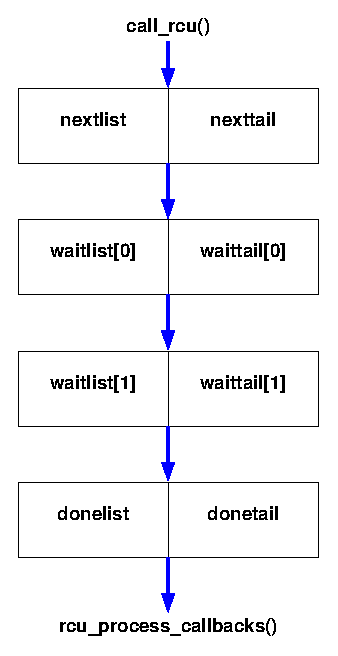
\includegraphics{appendix/rcuimpl/RCUpreemptLists}}
\end{center}
\caption{Preemptible RCU Callback Flow}
\label{app:rcuimpl:Preemptible RCU Callback Flow}
\end{figure}

Figure~\ref{app:rcuimpl:Preemptible RCU Callback Flow}
shows how RCU callbacks flow through a given
\co{rcu_data} structure's lists, from creation by
\co{call_rcu()} through invocation by
\co{rcu_process_callbacks()}.
Each blue arrow represents one pass by the grace-period state machine,
which is described in a later section.



\paragraph{{\tt rcu\_flipctr}}
\label{app:rcuimpl:rcu_flipctr}

As noted earlier, the \co{rcu_flipctr}
per-CPU array of counters contains the
counter pairs that track outstanding RCU read-side critical sections.
Any given counter in this array can go negative, for example, when
a task is migrated to a different CPU in the middle of an RCU
read-side critical section.
However, the sum of the counters will
still remain positive throughout the corresponding grace period, and will
furthermore go to zero at the end of that grace period.

\paragraph{{\tt rcu\_try\_flip\_state}}
\label{app:rcuimpl:rcu_try_flip_state}

The \co{rcu_try_flip_state} variable tracks the current state of
the grace-period state machine, as described in the next section.

\paragraph{{\tt rcu\_try\_flip\_flag}}
\label{app:rcuimpl:rcu_try_flip_flag}

The \co{rcu_try_flip_flag} per-CPU variable alerts the corresponding
CPU that the grace-period counter has recently been incremented, and
also records that CPU's acknowledgment.
Once a given CPU has acknowledged the counter flip, all subsequent actions
taken by \co{rcu_read_lock()} on that CPU must account for the
new value of the grace-period counter, in particular, when incrementing
\co{rcu_flipctr} in \co{rcu_read_lock()}.

\paragraph{{\tt rcu\_mb\_flag}}
\label{app:rcuimpl:rcu_mb_flag}

The \co{rcu_mb_flag} per-CPU variable alerts the corresponding
CPU that it must execute a memory barrier in order for the grace-period
state machine to proceed, and also records that CPU's acknowledgment.
Once a given CPU has executed its memory barrier, the memory operations
of all prior RCU read-side critical will be visible to any code sequenced
after the corresponding grace period.


\subsubsection{Grace-Period State Machine}
\label{app:rcuimpl:Grace-Period State Machine}

This section gives an overview of the states executed by the grace-period
state machine, and then walks through the relevant code.

\paragraph{Grace-Period State Machine Overview}
\label{app:rcuimpl:Grace-Period State Machine Overview}

The state (recorded in \co{rcu_try_flip_state})
can take on the following values:

\begin{itemize}
\item	\co{rcu_try_flip_idle_state}:  the grace-period state
	machine is idle due to there being no RCU grace-period activity.
	The \co{rcu_ctrlblk.completed} grace-period counter
	is incremented upon exit from this state, and all of the
	per-CPU \co{rcu_flip_flag} variables are set
	to \co{rcu_flipped}.
\item	\co{rcu_try_flip_waitack_state}:
	waiting for all CPUs to acknowledge that they have seen the
	previous state's increment, which they do by setting their
	\co{rcu_flip_flag} variables to \co{rcu_flip_seen}.
	Once all CPUs have so acknowledged, we know that the old
	set of counters can no longer be incremented.
\item	\co{rcu_try_flip_waitzero_state}:
	waiting for the old counters to sum to zero.
	Once the counters sum to zero, all of the per-CPU
	\co{rcu_mb_flag} variables are set to
	\co{rcu_mb_needed}.
\item	\co{rcu_try_flip_waitmb_state}:
	waiting for all CPUs to execute a memory-barrier instruction,
	which they signify by setting their \co{rcu_mb_flag}
	variables to \co{rcu_mb_done}.
	Once all CPUs have done so, all CPUs are guaranteed to see
	the changes made by any RCU read-side critical section that
	started before the beginning of the corresponding grace period,
	even on weakly ordered machines.
\end{itemize}

\begin{figure}[htb]
\begin{center}
\resizebox{3in}{!}{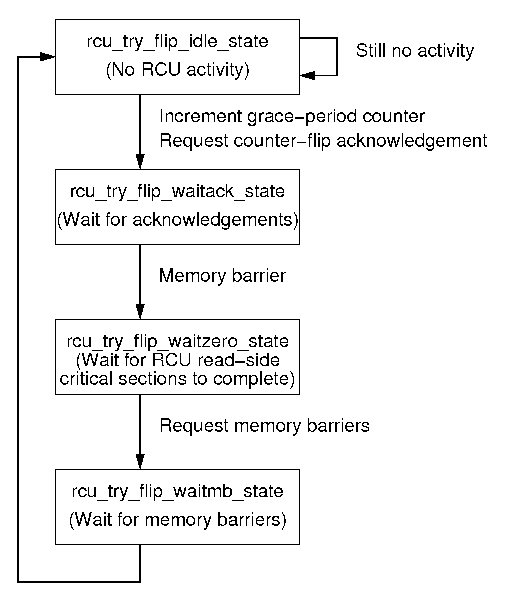
\includegraphics{appendix/rcuimpl/RCUpreemptStates}}
\end{center}
\caption{Preemptible RCU State Machine}
\label{app:rcuimpl:Preemptible RCU State Machine}
\end{figure}

The grace period state machine cycles through these states sequentially,
as shown in
Figure~\ref{app:rcuimpl:Preemptible RCU State Machine}.

\begin{figure}[htb]
\begin{center}
\resizebox{3in}{!}{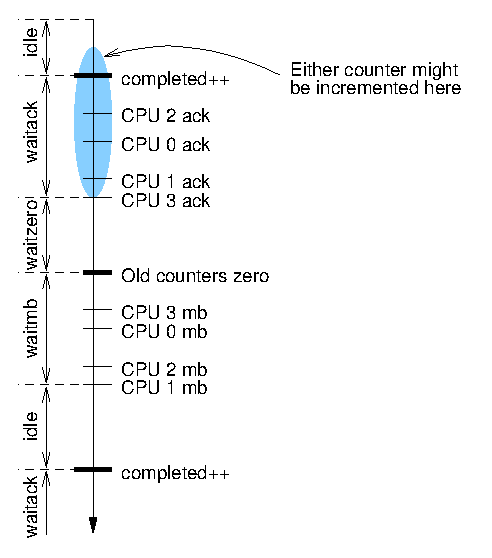
\includegraphics{appendix/rcuimpl/RCUpreemptTimeline}}
\end{center}
\caption{Preemptible RCU State Machine Timeline}
\label{app:rcuimpl:Preemptible RCU State Machine Timeline}
\end{figure}

Figure~\ref{app:rcuimpl:Preemptible RCU State Machine Timeline}
shows how the state machine operates over time.
The states are shown along the figure's left-hand side and the relevant events
are shown along the timeline, with time proceeding in the downward direction.
We will elaborate on this figure when we validate the algorithm in
a later section.

In the meantime, here are some important things to note:

\begin{enumerate}
\item	The increment of the \co{rcu_ctrlblk.completed} counter
	might be observed at different times by different CPUs, as
	indicated by the blue oval.  However, after a given
	CPU has acknowledged the increment, it is required to
	use the new counter.
	Therefore, once all CPUs have acknowledged, the old counter
	can only be decremented.
\item	A given CPU advances its callback lists just before
	acknowledging the counter increment.
\item	The blue oval represents the fact that memory reordering
	might cause different CPUs to see the increment at
	different times.
	This means that a given CPU might believe that some
	other CPU has jumped the gun, using the new value of the counter
	before the counter was actually incremented.
	In fact, in theory, a given CPU might see the next increment of the
	\co{rcu_ctrlblk.completed} counter as early as
	the last preceding memory barrier.
	(Note well that this sentence is very imprecise.
	If you intend to do correctness proofs involving memory barriers,
	please see Appendix~\ref{app:rcuimpl:Formal Validation}.
\item	Because \co{rcu_read_lock()} does not contain any
	memory barriers, the corresponding RCU read-side critical
	sections might be reordered by the CPU to follow the
	\co{rcu_read_unlock()}.
	Therefore, the memory barriers are required to ensure
	that the actions of the RCU read-side critical sections
	have in fact completed.
\item	As we will see, the fact that different CPUs can see the
	counter flip happening at different times means that a
	single trip through the state machine is not sufficient
	for a grace period: multiple trips are required.
\end{enumerate}

\paragraph{Grace-Period State Machine Walkthrough}
\label{app:rcuimpl:Grace-Period State Machine Walkthrough}

\begin{figure}[tbp]
{ \scriptsize
\begin{verbatim}
  1 void rcu_check_callbacks(int cpu, int user)
  2 {
  3   unsigned long flags;
  4   struct rcu_data *rdp = RCU_DATA_CPU(cpu);
  5
  6   rcu_check_mb(cpu);
  7   if (rcu_ctrlblk.completed == rdp->completed)
  8     rcu_try_flip();
  9   spin_lock_irqsave(&rdp->lock, flags);
 10   RCU_TRACE_RDP(rcupreempt_trace_check_callbacks, rdp);
 11   __rcu_advance_callbacks(rdp);
 12   spin_unlock_irqrestore(&rdp->lock, flags);
 13 }
\end{verbatim}
}
\caption{{\tt rcu\_check\_callbacks()} Implementation}
\label{fig:app:rcuimpl:rcu_check_callbacks() Implementation}
\end{figure}

This section walks through the C code that implements the RCU
grace-period state machine, which is invoked from the scheduling-clock
interrupt, which invokes \co{rcu_check_callbacks()} with
irqs (and thus also preemption) disabled.
This function is implemented as shown in
Figure~\ref{fig:app:rcuimpl:rcu_check_callbacks() Implementation}.
Line~4 selects the \co{rcu_data} structure corresponding
to the current CPU, and line~6 checks to see if this CPU needs
to execute a memory barrier to advance the state machine out of the
\co{rcu_try_flip_waitmb_state} state.
Line~7 checks to see if this CPU is already aware of the
current grace-period stage number, and line~8 attempts to advance the
state machine if so.
Lines~9 and 12 hold the \co{rcu_data}'s lock, and
line~11 advances callbacks if appropriate.
Line~10 updates RCU tracing statistics, if enabled via
\co{CONFIG_RCU_TRACE}.

\begin{figure}[tbp]
{ \scriptsize
\begin{verbatim}
  1 static void rcu_check_mb(int cpu)
  2 {
  3   if (per_cpu(rcu_mb_flag, cpu) == rcu_mb_needed) {
  4     smp_mb();
  5     per_cpu(rcu_mb_flag, cpu) = rcu_mb_done;
  6   }
  7 }
\end{verbatim}
}
\caption{{\tt rcu\_check\_mb()} Implementation}
\label{fig:app:rcuimpl:rcu_check_mb() Implementation}
\end{figure}

The \co{rcu_check_mb()} function executes a memory barrier
as needed as shown in
Figure~\ref{fig:app:rcuimpl:rcu_check_mb() Implementation}.
Line~3 checks to see if this CPU needs to execute a memory barrier,
and, if so, line~4 executes one and line~5 informs the state
machine.
Note that this memory barrier ensures that any CPU that sees the new
value of \co{rcu_mb_flag} will also see the memory operations
executed by this CPU in any prior RCU read-side critical section.

\begin{figure}[tbp]
{ \scriptsize
\begin{verbatim}
  1 static void rcu_try_flip(void)
  2 {
  3   unsigned long flags;
  4
  5   RCU_TRACE_ME(rcupreempt_trace_try_flip_1);
  6   if (!spin_trylock_irqsave(&rcu_ctrlblk.fliplock, flags)) {
  7     RCU_TRACE_ME(rcupreempt_trace_try_flip_e1);
  8     return;
  9   }
 10   switch (rcu_try_flip_state) {
 11   case rcu_try_flip_idle_state:
 12     if (rcu_try_flip_idle())
 13       rcu_try_flip_state = rcu_try_flip_waitack_state;
 14     break;
 15   case rcu_try_flip_waitack_state:
 16     if (rcu_try_flip_waitack())
 17       rcu_try_flip_state = rcu_try_flip_waitzero_state;
 18     break;
 19   case rcu_try_flip_waitzero_state:
 20     if (rcu_try_flip_waitzero())
 21       rcu_try_flip_state = rcu_try_flip_waitmb_state;
 22     break;
 23   case rcu_try_flip_waitmb_state:
 24     if (rcu_try_flip_waitmb())
 25       rcu_try_flip_state = rcu_try_flip_idle_state;
 26   }
 27   spin_unlock_irqrestore(&rcu_ctrlblk.fliplock, flags);
 28 }
\end{verbatim}
}
\caption{{\tt rcu\_try\_flip()} Implementation}
\label{fig:app:rcuimpl:rcu_try_flip() Implementation}
\end{figure}

The \co{rcu_try_flip()} function implements the top level of
the RCU grace-period state machine, as shown in
Figure~\ref{fig:app:rcuimpl:rcu_try_flip() Implementation}.
Line~6 attempts to acquire the global RCU state-machine lock,
and returns if unsuccessful.
Lines;~5 and 7 accumulate RCU-tracing statistics (again, if
\co{CONFIG_RCU_TRACE} is enabled).
Lines~10 through 26 execute the state machine,
each invoking a function specific to that state.
Each such function returns 1 if the state needs to be advanced and
0 otherwise.
In principle, the next state could be executed immediately,
but in practice we choose not to do so in order to reduce latency.
Finally, line~27 releases the global RCU state-machine lock
that was acquired by line~6.

\begin{figure}[tbp]
{ \scriptsize
\begin{verbatim}
  1 static int rcu_try_flip_idle(void)
  2 {
  3   int cpu;
  4
  5   RCU_TRACE_ME(rcupreempt_trace_try_flip_i1);
  6   if (!rcu_pending(smp_processor_id())) {
  7     RCU_TRACE_ME(rcupreempt_trace_try_flip_ie1);
  8     return 0;
  9   }
 10   RCU_TRACE_ME(rcupreempt_trace_try_flip_g1);
 11   rcu_ctrlblk.completed++;
 12   smp_mb();
 13   for_each_cpu_mask(cpu, rcu_cpu_online_map)
 14     per_cpu(rcu_flip_flag, cpu) = rcu_flipped;
 15   return 1;
 16 }
\end{verbatim}
}
\caption{{\tt rcu\_try\_flip\_idle()} Implementation}
\label{fig:app:rcuimpl:rcu_try_flip_idle() Implementation}
\end{figure}

The \co{rcu_try_flip_idle()} function is called when the
RCU grace-period state machine is idle, and is thus responsible for
getting it started when needed.
Its code is shown in
Figure~\ref{fig:app:rcuimpl:rcu_try_flip_idle() Implementation}.
Line~6 checks to see if there is any RCU grace-period work
pending for this CPU, and if not, line~8 leaves, telling
the top-level state machine to remain in the idle state.
If instead there is work to do, line~11 increments the
grace-period stage counter, line~12 does a memory barrier
to ensure that CPUs see the new counter before they see the
request to acknowledge it, and lines~13 and 14 set all of
the online CPUs' \co{rcu_flip_flag}.
Finally, line~15 tells the top-level state machine to
advance to the next state.

\begin{figure}[tbp]
{ \scriptsize
\begin{verbatim}
  1 static int rcu_try_flip_waitack(void)
  2 {
  3   int cpu;
  4
  5   RCU_TRACE_ME(rcupreempt_trace_try_flip_a1);
  6   for_each_cpu_mask(cpu, rcu_cpu_online_map)
  7     if (per_cpu(rcu_flip_flag, cpu) != rcu_flip_seen) {
  8       RCU_TRACE_ME(rcupreempt_trace_try_flip_ae1);
  9       return 0;
 10     }
 11   smp_mb();
 12   RCU_TRACE_ME(rcupreempt_trace_try_flip_a2);
 13   return 1;
 14 }
\end{verbatim}
}
\caption{{\tt rcu\_try\_flip\_waitack()} Implementation}
\label{fig:app:rcuimpl:rcu_try_flip_waitack() Implementation}
\end{figure}

The \co{rcu_try_flip_waitack()} function, shown in
Figure~\ref{fig:app:rcuimpl:rcu_try_flip_waitack() Implementation},
checks to see
if all online CPUs have acknowledged the counter flip (AKA ``increment'',
but called ``flip'' because the bottom bit, which \co{rcu_read_lock()}
uses to index the \co{rcu_flipctr} array, \emph{does} flip).
If they have, it tells the top-level grace-period state machine to
move to the next state.

Line~6 cycles through all of the online CPUs, and line~7
checks to see if the current such CPU has acknowledged the last counter
flip.
If not, line~9 tells the top-level grace-period state machine to
remain in this state.
Otherwise, if all online CPUs have acknowledged, then line~11
does a memory barrier to ensure that we don't check for zeroes before
the last CPU acknowledges.
This may seem dubious, but CPU designers have sometimes done strange
things.
Finally, line~13 tells the top-level grace-period state machine
to advance to the next state.

\begin{figure}[tbp]
{ \scriptsize
\begin{verbatim}
  1 static int rcu_try_flip_waitzero(void)
  2 {
  3   int cpu;
  4   int lastidx = !(rcu_ctrlblk.completed & 0x1);
  5   int sum = 0;
  6
  7   RCU_TRACE_ME(rcupreempt_trace_try_flip_z1);
  8   for_each_possible_cpu(cpu)
  9     sum += per_cpu(rcu_flipctr, cpu)[lastidx];
 10   if (sum != 0) {
 11     RCU_TRACE_ME(rcupreempt_trace_try_flip_ze1);
 12     return 0;
 13   }
 14   smp_mb();
 15   for_each_cpu_mask(cpu, rcu_cpu_online_map)
 16     per_cpu(rcu_mb_flag, cpu) = rcu_mb_needed;
 17   RCU_TRACE_ME(rcupreempt_trace_try_flip_z2);
 18   return 1;
 19 }
\end{verbatim}
}
\caption{{\tt rcu\_try\_flip\_waitzero()} Implementation}
\label{fig:app:rcuimpl:rcu_try_flip_waitzero() Implementation}
\end{figure}

The \co{rcu_try_flip_waitzero()} function, shown in
Figure~\ref{fig:app:rcuimpl:rcu_try_flip_waitzero() Implementation},
checks to see if
all pre-existing RCU read-side critical sections have completed,
telling the state machine to advance if so.
Lines~8 and 9 sum the counters, and line~10 checks
to see if the result is zero, and, if not, line~12 tells
the state machine to stay right where it is.
Otherwise, line~14 executes a memory barrier to ensure that
no CPU sees the subsequent call for a memory barrier before it
has exited its last RCU read-side critical section.
This possibility might seem remote, but again, CPU designers have
done stranger things, and besides, this is anything but a fastpath.
Lines~15 and 16 set all online CPUs' \co{rcu_mb_flag}
variables, and line~18 tells the state machine to advance to
the next state.

\begin{figure}[tbp]
{ \scriptsize
\begin{verbatim}
  1 static int rcu_try_flip_waitmb(void)
  2 {
  3   int cpu;
  4
  5   RCU_TRACE_ME(rcupreempt_trace_try_flip_m1);
  6   for_each_cpu_mask(cpu, rcu_cpu_online_map)
  7     if (per_cpu(rcu_mb_flag, cpu) != rcu_mb_done) {
  8       RCU_TRACE_ME(rcupreempt_trace_try_flip_me1);
  9       return 0;
 10     }
 11   smp_mb();
 12   RCU_TRACE_ME(rcupreempt_trace_try_flip_m2);
 13   return 1;
 14 }
\end{verbatim}
}
\caption{{\tt rcu\_try\_flip\_waitmb()} Implementation}
\label{fig:app:rcuimpl:rcu_try_flip_waitmb() Implementation}
\end{figure}

The \co{rcu_try_flip_waitmb()} function, shown in
Figure~\ref{fig:app:rcuimpl:rcu_try_flip_waitmb() Implementation},
checks to see
if all online CPUs have executed the requested memory barrier,
telling the state machine to advance if so.
Lines~6 and 7 check each online CPU to see if it has
done the needed memory barrier, and if not, line~9 tells
the state machine not to advance.
Otherwise, if all CPUs have executed a memory barrier, line~11
executes a memory barrier to ensure that any RCU callback invocation
follows all of the memory barriers, and line~13 tells the
state machine to advance.

\begin{figure}[tbp]
{ \scriptsize
\begin{verbatim}
  1 static void __rcu_advance_callbacks(struct rcu_data *rdp)
  2 {
  3   int cpu;
  4   int i;
  5   int wlc = 0;
  6
  7   if (rdp->completed != rcu_ctrlblk.completed) {
  8     if (rdp->waitlist[GP_STAGES - 1] != NULL) {
  9       *rdp->donetail = rdp->waitlist[GP_STAGES - 1];
 10       rdp->donetail = rdp->waittail[GP_STAGES - 1];
 11       RCU_TRACE_RDP(rcupreempt_trace_move2done, rdp);
 12     }
 13     for (i = GP_STAGES - 2; i >= 0; i--) {
 14       if (rdp->waitlist[i] != NULL) {
 15         rdp->waitlist[i + 1] = rdp->waitlist[i];
 16         rdp->waittail[i + 1] = rdp->waittail[i];
 17         wlc++;
 18       } else {
 19         rdp->waitlist[i + 1] = NULL;
 20         rdp->waittail[i + 1] =
 21           &rdp->waitlist[i + 1];
 22       }
 23     }
 24     if (rdp->nextlist != NULL) {
 25       rdp->waitlist[0] = rdp->nextlist;
 26       rdp->waittail[0] = rdp->nexttail;
 27       wlc++;
 28       rdp->nextlist = NULL;
 29       rdp->nexttail = &rdp->nextlist;
 30       RCU_TRACE_RDP(rcupreempt_trace_move2wait, rdp);
 31     } else {
 32       rdp->waitlist[0] = NULL;
 33       rdp->waittail[0] = &rdp->waitlist[0];
 34     }
 35     rdp->waitlistcount = wlc;
 36     rdp->completed = rcu_ctrlblk.completed;
 37   }
 38   cpu = raw_smp_processor_id();
 39   if (per_cpu(rcu_flip_flag, cpu) == rcu_flipped) {
 40     smp_mb();
 41     per_cpu(rcu_flip_flag, cpu) = rcu_flip_seen;
 42     smp_mb();
 43   }
 44 }
\end{verbatim}
}
\caption{{\tt \_\_rcu\_advance\_callbacks()} Implementation}
\label{fig:app:rcuimpl:__rcu_advance_callbacks() Implementation}
\end{figure}

The \co{__rcu_advance_callbacks()} function, shown in
Figure~\ref{fig:app:rcuimpl:__rcu_advance_callbacks() Implementation},
advances callbacks and acknowledges the counter flip.
Line~7 checks to see if the global \co{rcu_ctrlblk.completed}
counter has advanced since the last call by the current CPU to this
function.
If not, callbacks need not be advanced (lines~8-37).
Otherwise, lines~8 through 37 advance callbacks through the lists
(while maintaining a count of the number of non-empty lists in the
\co{wlc} variable).
In either case, lines~38 through 43 acknowledge the counter flip
if needed.

\QuickQuiz{}
	How is it possible for lines~38-43 of
	\co{__rcu_advance_callbacks()} to be executed when
	lines~7-37 have not?
	Won't they both be executed just after a counter flip, and
	never at any other time?
\QuickQuizAnswer{
	Consider the following sequence of events:
	\begin{enumerate}
	\item	CPU 0 executes lines~5-12 of
		\co{rcu_try_flip_idle()}.
	\item	CPU 1 executes \co{__rcu_advance_callbacks()}.
		Because \co{rcu_ctrlblk.completed} has been
		incremented, lines~7-37 execute.
		However, none of the \co{rcu_flip_flag} variables
		have been set, so lines~38-43 do \emph{not} execute.
	\item	CPU 0 executes lines~13-15 of
		\co{rcu_try_flip_idle()}.
	\item	Later, CPU 1 again executes \co{__rcu_advance_callbacks()}.
		The counter has not been incremented since the earlier
		execution, but the \co{rcu_flip_flag} variables have
		all been set, so only lines~38-43 are executed.
	\end{enumerate}
} \QuickQuizEnd


\subsubsection{Read-Side Primitives}
\label{app:rcuimpl:Read-Side Primitives}

This section examines the \co{rcu_read_lock()} and
\co{rcu_read_unlock()} primitives, followed by a
discussion of how this implementation deals with the fact
that these two primitives do not contain memory barriers.

\paragraph{{\tt rcu\_read\_lock()}}
\label{app:rcuimpl:rcu_read_lock()}

\begin{figure}[tbp]
{ \scriptsize
\begin{verbatim}
  1 void __rcu_read_lock(void)
  2 {
  3   int idx;
  4   struct task_struct *t = current;
  5   int nesting;
  6
  7   nesting = ACCESS_ONCE(t->rcu_read_lock_nesting);
  8   if (nesting != 0) {
  9     t->rcu_read_lock_nesting = nesting + 1;
 10   } else {
 11     unsigned long flags;
 12
 13     local_irq_save(flags);
 14     idx = ACCESS_ONCE(rcu_ctrlblk.completed) & 0x1;
 15     ACCESS_ONCE(__get_cpu_var(rcu_flipctr)[idx])++;
 16     ACCESS_ONCE(t->rcu_read_lock_nesting) = nesting + 1;
 17     ACCESS_ONCE(t->rcu_flipctr_idx) = idx;
 18     local_irq_restore(flags);
 19   }
 20 }
\end{verbatim}
}
\caption{{\tt \_\_rcu\_read\_lock()} Implementation}
\label{fig:app:rcuimpl:__rcu_read_lock() Implementation}
\end{figure}

The implementation of \co{rcu_read_lock()} is as shown in
Figure~\ref{fig:app:rcuimpl:__rcu_read_lock() Implementation}.
Line~7 fetches this task's RCU read-side critical-section nesting
counter.
If line~8 finds that this counter is non-zero,
then we are already protected by an outer
\co{rcu_read_lock()}, in which case line~9 simply increments
this counter.

However, if this is the outermost \co{rcu_read_lock()},
then more work is required.
Lines~13 and 18 suppress and restore irqs to ensure that the
intervening code is neither preempted nor interrupted by a
scheduling-clock interrupt (which runs the grace period state machine).
Line~14 fetches the grace-period counter,
line~15 increments the current counter for
this CPU, line~16 increments the nesting counter,
and line~17 records the old/new counter index so that
\co{rcu_read_unlock()} can decrement the corresponding
counter (but on whatever CPU it ends up running on).

The \co{ACCESS_ONCE()} macros force the compiler to
emit the accesses in order.
Although this does not prevent the CPU from reordering the accesses
from the viewpoint of other CPUs, it does ensure that NMI and
SMI handlers running on this CPU will see these accesses in order.
This is critically important:

\begin{enumerate}
\item	In absence of the \co{ACCESS_ONCE()} in the assignment
	to \co{idx}, the compiler would be within its rights
	to: (a) eliminate the local variable \co{idx} and
	(b) compile the increment on line~16 as a
	fetch-increment-store sequence, doing separate accesses to
	\co{rcu_ctrlblk.completed} for the fetch and the
	store.
	If the value of \co{rcu_ctrlblk.completed} had
	changed in the meantime, this would corrupt the
	\co{rcu_flipctr} values.
\item	If the assignment to \co{rcu_read_lock_nesting}
	(line~17) were to be reordered to precede the increment
	of \co{rcu_flipctr} (line~16), and if an
	NMI occurred between these two events, then an
	\co{rcu_read_lock()} in that NMI's handler
	would incorrectly conclude that it was already under the
	protection of \co{rcu_read_lock()}.
\item	If the assignment to \co{rcu_read_lock_nesting}
        (line~17) were to be reordered to follow the assignment
	to \co{rcu_flipctr_idx} (line~18), and if an
	NMI occurred between these two events, then an
	\co{rcu_read_lock()} in that NMI's handler
	would clobber \co{rcu_flipctr_idx}, possibly
	causing the matching \co{rcu_read_unlock()} to
	decrement the wrong counter.
	This in turn could result in premature ending of a
	grace period, indefinite extension of a grace period,
	or even both.
\end{enumerate}

It is not clear that the \co{ACCESS_ONCE} on the assignment to
\co{nesting} (line~7) is required.
It is also unclear whether the \co{smp_read_barrier_depends()}
(line~15) is needed: it was added to ensure that changes to index
and value remain ordered.

The reasons that irqs must be disabled from line~13 through
line~19 are as follows:

\begin{enumerate}
\item	Suppose one CPU loaded \co{rcu_ctrlblk.completed}
	(line~14), then a second CPU incremented this counter,
	and then the first CPU took a scheduling-clock interrupt.
	The first CPU would then see that it needed to acknowledge
	the counter flip, which it would do.
	This acknowledgment is a promise to avoid incrementing
	the newly old counter, and this CPU would break this
	promise.
	Worse yet, this CPU might be preempted immediately upon
	return from the scheduling-clock interrupt, and thus
	end up incrementing the counter at some random point
	in the future.
	Either situation could disrupt grace-period detection.
\item	Disabling irqs has the side effect of disabling preemption.
	If this code were to be preempted between fetching
	\co{rcu_ctrlblk.completed} (line~14) and
	incrementing \co{rcu_flipctr} (line~16),
	it might well be migrated to some other CPU.
	This would result in it non-atomically incrementing
	the counter from that other CPU.
	If this CPU happened to be executing in \co{rcu_read_lock()}
	or \co{rcu_read_unlock()} just at that time, one
	of the increments or decrements might be lost, again
	disrupting grace-period detection.
	The same result could happen on RISC machines if the preemption
	occurred in the middle of the increment (after the fetch of
	the old counter but before the store of the newly incremented
	counter).
\item	Permitting preemption in the midst
	of line~16, between selecting the current CPU's copy
	of the \co{rcu_flipctr} array and the increment of
	the element indicated by \co{rcu_flipctr_idx}, can
	result in a similar failure.
	Execution might well resume on some other CPU.
	If this resumption happened concurrently with an
	\co{rcu_read_lock()} or \co{rcu_read_unlock()}
	running on the original CPU,
	an increment or decrement might be lost, resulting in either
	premature termination of a grace period, indefinite extension
	of a grace period, or even both.
\item	Failing to disable preemption can also defeat RCU priority
	boosting, which relies on \co{rcu_read_lock_nesting}
	to determine when a given task is in an RCU read-side
	critical section.
	So, for example, if a given task is indefinitely
	preempted just after incrementing \co{rcu_flipctr},
	but before updating \co{rcu_read_lock_nesting},
	then it will stall RCU grace periods for as long as it
	is preempted.
	However, because \co{rcu_read_lock_nesting} has not
	yet been incremented, the RCU priority booster has no way
	to tell that boosting is needed.
	Therefore, in the presence of CPU-bound realtime threads,
	the preempted task might stall grace periods indefinitely,
	eventually causing an OOM event.
\end{enumerate}

The last three reasons could of course be addressed by disabling
preemption rather than disabling of irqs, but given that the first
reason requires disabling irqs in any case, there is little reason
to separately disable preemption.
It is entirely possible that the first reason might be tolerated
by requiring an additional grace-period stage, however, it is not
clear that disabling preemption is much faster than disabling
interrupts on modern CPUs.

\paragraph{{\tt rcu\_read\_unlock()}}
\label{app:rcuimpl:rcu_read_unlock()}

\begin{figure}[tbp]
{ \scriptsize
\begin{verbatim}
  1 void __rcu_read_unlock(void)
  2 {
  3   int idx;
  4   struct task_struct *t = current;
  5   int nesting;
  6
  7   nesting = ACCESS_ONCE(t->rcu_read_lock_nesting);
  8   if (nesting > 1) {
  9     t->rcu_read_lock_nesting = nesting - 1;
 10   } else {
 11     unsigned long flags;
 12
 13     local_irq_save(flags);
 14     idx = ACCESS_ONCE(t->rcu_flipctr_idx);
 15     ACCESS_ONCE(t->rcu_read_lock_nesting) = nesting - 1;
 16     ACCESS_ONCE(__get_cpu_var(rcu_flipctr)[idx])--;
 17     local_irq_restore(flags);
 18   }
 19 }
\end{verbatim}
}
\caption{{\tt \_\_rcu\_read\_unlock()} Implementation}
\label{fig:app:rcuimpl:__rcu_read_unlock() Implementation}
\end{figure}

The implementation of \co{rcu_read_unlock()} is shown in
Figure~\ref{fig:app:rcuimpl:__rcu_read_unlock() Implementation}.
Line~7 fetches the \co{rcu_read_lock_nesting} counter,
which line~8 checks to see if we are under the protection of an
enclosing \co{rcu_read_lock()} primitive.
If so, line~9 simply decrements the counter.

However, as with \co{rcu_read_lock()}, we otherwise must do
more work.
Lines~13 and 17 disable and restore irqs in order to prevent
the scheduling-clock interrupt from invoking the grace-period state machine
while in the midst of \co{rcu_read_unlock()} processing.
Line~14 picks up the \co{rcu_flipctr_idx} that was
saved by the matching \co{rcu_read_lock()},
line~15
decrements \co{rcu_read_lock_nesting} so that irq and
NMI/SMI handlers will henceforth update \co{rcu_flipctr},
line~16 decrements the counter (with the same index as, but possibly
on a different CPU than, that incremented by the matching
\co{rcu_read_lock()}.

The \co{ACCESS_ONCE()} macros and irq disabling
are required for similar reasons that they are in
\co{rcu_read_lock()}.

\QuickQuiz{}
	What problems could arise if the lines containing
	\co{ACCESS_ONCE()} in \co{rcu_read_unlock()}
	were reordered by the compiler?
\QuickQuizAnswer{
	\begin{enumerate}
	\item	If the \co{ACCESS_ONCE()} were omitted from the
		fetch of \co{rcu_flipctr_idx} (line~14), then the compiler
		would be within its rights to eliminate \co{idx}.
		It would also be free to compile the \co{rcu_flipctr}
		decrement as a fetch-increment-store sequence, separately
		fetching \co{rcu_flipctr_idx} for both the fetch and
		the store.
		If an NMI were to occur between the fetch and the store, and
		if the NMI handler contained an \co{rcu_read_lock()},
		then the value of \co{rcu_flipctr_idx} would change
		in the meantime, resulting in corruption of the
		\co{rcu_flipctr} values, destroying the ability
		to correctly identify grace periods.
	\item	Another failure that could result from omitting the
		\co{ACCESS_ONCE()} from line~14 is due to
		the compiler reordering this statement to follow the
		decrement of \co{rcu_read_lock_nesting}
		(line~16).
		In this case, if an NMI were to occur between these two
		statements, then any \co{rcu_read_lock()} in the
		NMI handler could corrupt \co{rcu_flipctr_idx},
		causing the wrong \co{rcu_flipctr} to be
		decremented.
		As with the analogous situation in \co{rcu_read_lock()},
		this could result in premature grace-period termination,
		an indefinite grace period, or even both.
	\item	If \co{ACCESS_ONCE()} macros were omitted such that
		the update of \co{rcu_read_lock_nesting} could be
		interchanged by the compiler with the decrement of
		\co{rcu_flipctr}, and if an NMI occurred in between,
		any \co{rcu_read_lock()} in the NMI handler would
		incorrectly conclude that it was protected by an enclosing
		\co{rcu_read_lock()}, and fail to increment the
		\co{rcu_flipctr} variables.
	\end{enumerate}

	It is not clear that the \co{ACCESS_ONCE()} on the
	fetch of \co{rcu_read_lock_nesting} (line~7) is required.
} \QuickQuizEnd

\QuickQuiz{}
	What problems could arise if the lines containing
	\co{ACCESS_ONCE()} in \co{rcu_read_unlock()}
	were reordered by the CPU?
\QuickQuizAnswer{
	Absolutely none!  The code in \co{rcu_read_unlock()}
	interacts with the scheduling-clock interrupt handler
	running on the same CPU, and is thus insensitive to reorderings
	because CPUs always see their own accesses as if they occurred
	in program order.
	Other CPUs do access the \co{rcu_flipctr}, but because these
	other CPUs don't access any of the other variables, ordering is
	irrelevant.
} \QuickQuizEnd

\QuickQuiz{}
	What problems could arise in
	\co{rcu_read_unlock()} if irqs were not disabled?
\QuickQuizAnswer{
	\begin{enumerate}
	\item	Disabling irqs has the side effect of disabling preemption.
		Suppose that this code were to be preempted in the midst
		of line~17 between selecting the current CPU's copy
		of the \co{rcu_flipctr} array and the decrement of
		the element indicated by \co{rcu_flipctr_idx}.
		Execution might well resume on some other CPU.
		If this resumption happened concurrently with an
		\co{rcu_read_lock()} or \co{rcu_read_unlock()}
		running on the original CPU,
		an increment or decrement might be lost, resulting in either
		premature termination of a grace period, indefinite extension
		of a grace period, or even both.
	\item	Failing to disable preemption can also defeat RCU priority
		boosting, which relies on \co{rcu_read_lock_nesting}
		to determine which tasks to boost.
		If preemption occurred between the update of
		\co{rcu_read_lock_nesting} (line~16) and of
		\co{rcu_flipctr} (line~17), then a grace
		period might be stalled until this task resumed.
		But because the RCU priority booster has no way of knowing
		that this particular task is stalling grace periods, needed
		boosting will never occur.
		Therefore, if there are CPU-bound realtime tasks running,
		the preempted task might never resume, stalling grace periods
		indefinitely, and eventually resulting in OOM.
	\end{enumerate}

	Of course, both of these situations could be handled by disabling
	preemption rather than disabling irqs.
	(The CPUs I have access to do not show much difference between these
	two alternatives, but others might.)
} \QuickQuizEnd

\paragraph{Memory-Barrier Considerations}
\label{app:rcuimpl:Memory-Barrier Considerations}

\begin{figure}[htb]
\begin{center}
\resizebox{3in}{!}{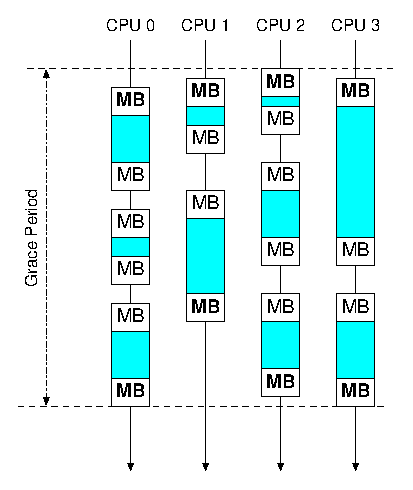
\includegraphics{appendix/rcuimpl/RCUrt-MBwaste}}
\end{center}
\caption{Preemptible RCU with Read-Side Memory Barriers}
\label{app:rcuimpl:Preemptible RCU with Read-Side Memory Barriers}
\end{figure}

Note that these two primitives contains no memory barriers, so there is
nothing to stop the CPU from executing the critical section
before executing the \co{rcu_read_lock()} or after executing
the \co{rcu_read_unlock()}.
The purpose of the \co{rcu_try_flip_waitmb_state} is to
account for this possible reordering, but only at the beginning or end of
a grace period.
To see why this approach is helpful, consider
Figure~\ref{app:rcuimpl:Preemptible RCU with Read-Side Memory Barriers},
which shows the wastefulness of the conventional approach of placing
a memory barrier at the beginning and end of each RCU read-side critical
section~\cite{PaulEMcKenney2006b}.

\begin{figure}[htb]
\begin{center}
\resizebox{3in}{!}{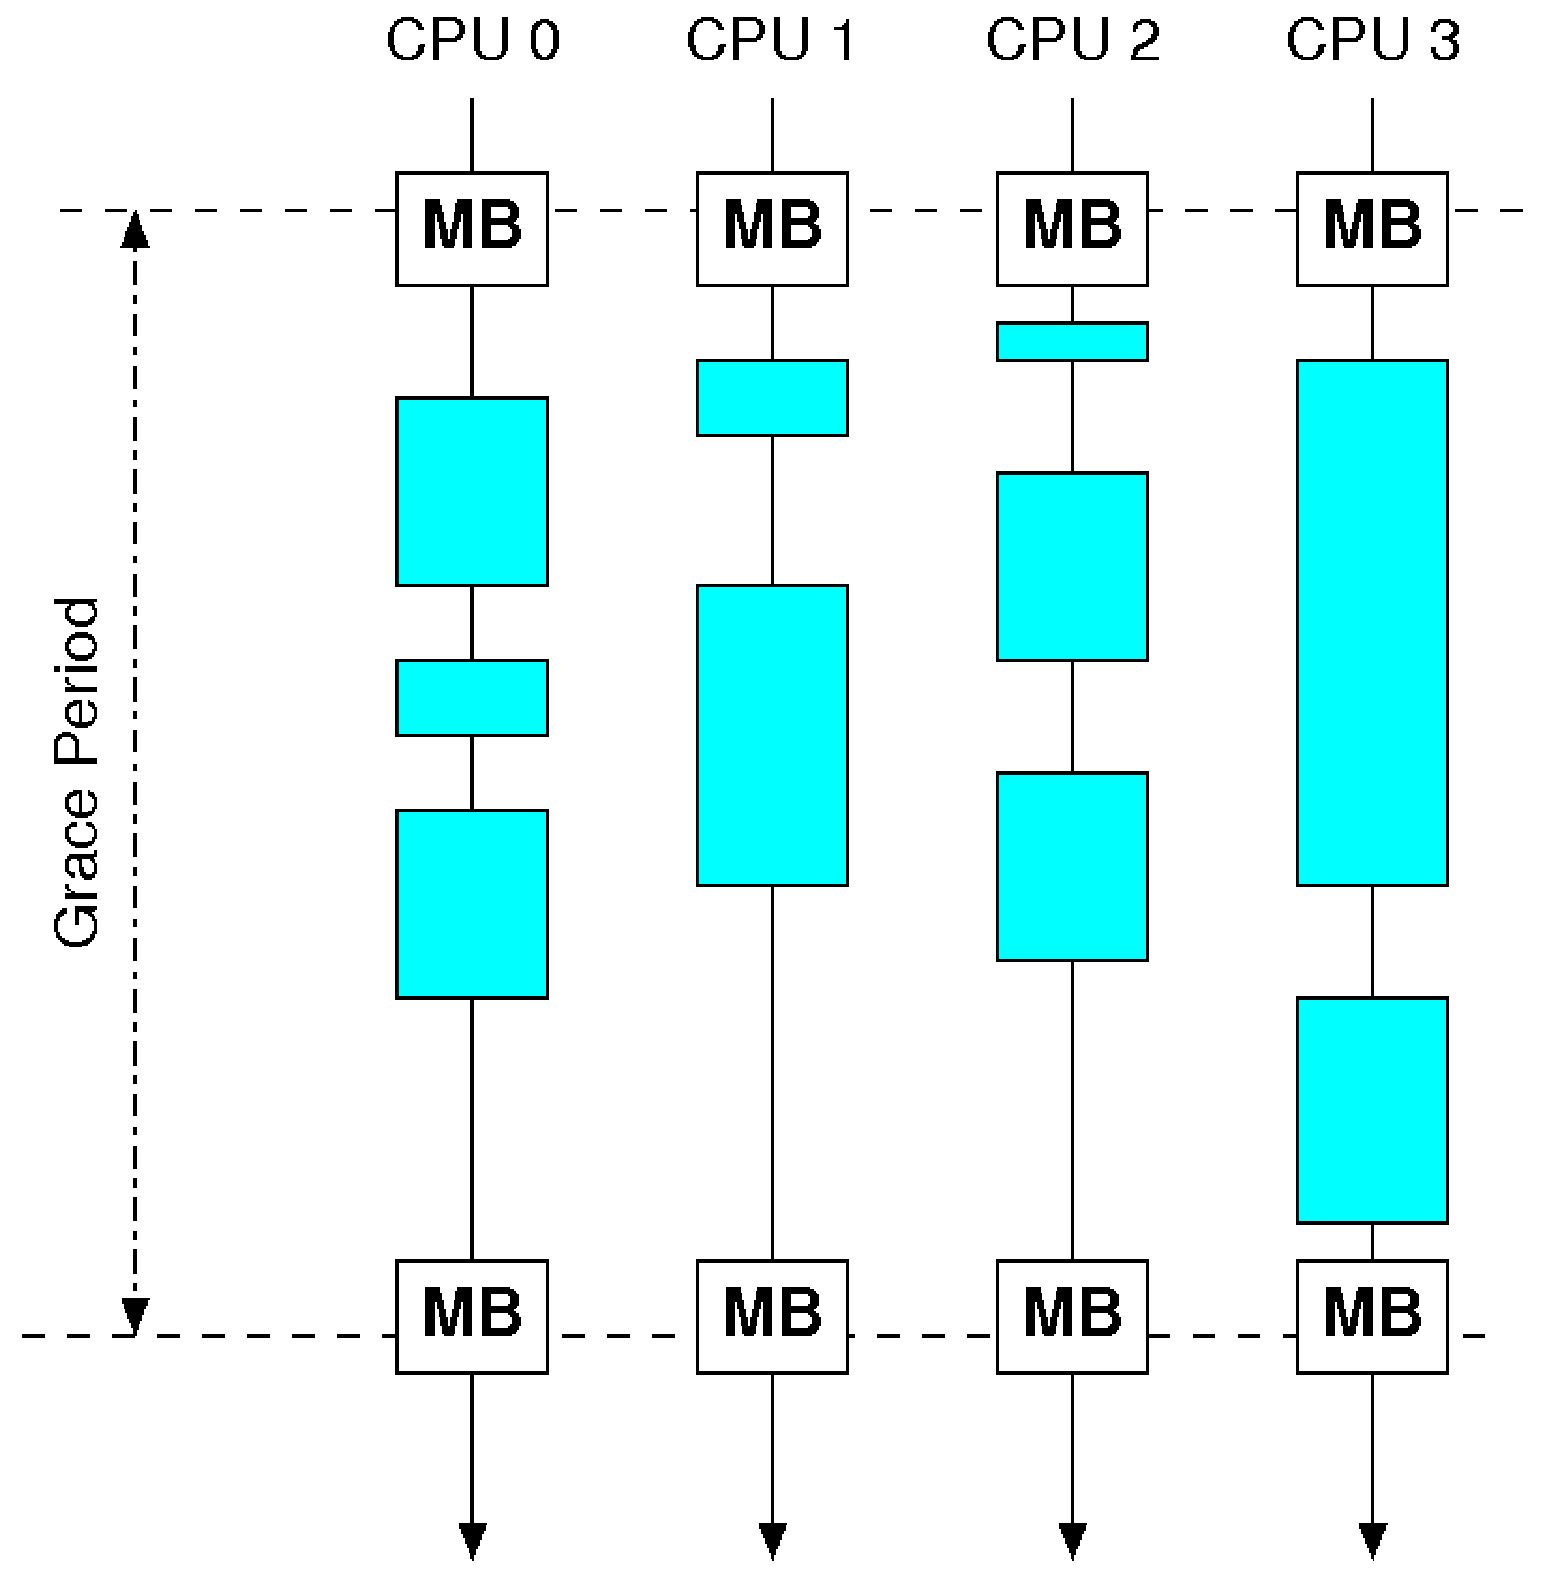
\includegraphics{appendix/rcuimpl/RCUrt-MBnowaste}}
\end{center}
\caption{Preemptible RCU with Grace-Period Memory Barriers}
\label{app:rcuimpl:Preemptible RCU with Grace-Period Memory Barriers}
\end{figure}

The ``MB''s represent memory barriers, and only the emboldened
barriers are needed, namely the first and last on a given CPU
for each grace period.
This preemptible RCU implementation therefore associates the memory
barriers with the grace period, as shown in
Figure~\ref{app:rcuimpl:Preemptible RCU with Grace-Period Memory Barriers}.

Given that the Linux kernel can execute literally millions of RCU
read-side critical sections per grace period, this latter approach
can result in substantial read-side savings, due to the fact that it
amortizes the cost of the memory barrier over all the read-side critical
sections in a grace period.

\subsection{Validation of Preemptible RCU}
\label{app:rcuimpl:Validation of Preemptible RCU}

\subsubsection{Testing}
\label{app:rcuimpl:Testing}

The preemptible RCU algorithm was tested with a two-stage grace period
on weakly ordered POWER4 and POWER5 CPUs using rcutorture running for
more than 24 hours on each machine, with 15M and 20M grace periods,
respectively, and with no errors.
Of course, this in no way proves that this algorithm is correct.
At most, it shows either that these two machines were extremely
lucky or that any bugs remaining in preemptible RCU have an extremely
low probability of occurring.
We therefore required additional assurance that this algorithm works,
or, alternatively, identification of remaining bugs.

This task requires a conceptual approach,
which is taken in the next section.

\subsubsection{Conceptual Validation}
\label{app:rcuimpl:Conceptual Validation}

Because neither \co{rcu_read_lock()} nor \co{rcu_read_unlock()}
contain memory barriers, the RCU read-side critical section can bleed
out on weakly ordered machines.
In addition, the relatively loose coupling of this RCU implementation
permits CPUs to disagree on when a given grace period starts and ends.
This leads to the question as to how long a given RCU read-side critical
section can possibly extend relative to the grace-period state machine.

\begin{figure}[htb]
\begin{center}
\resizebox{3in}{!}{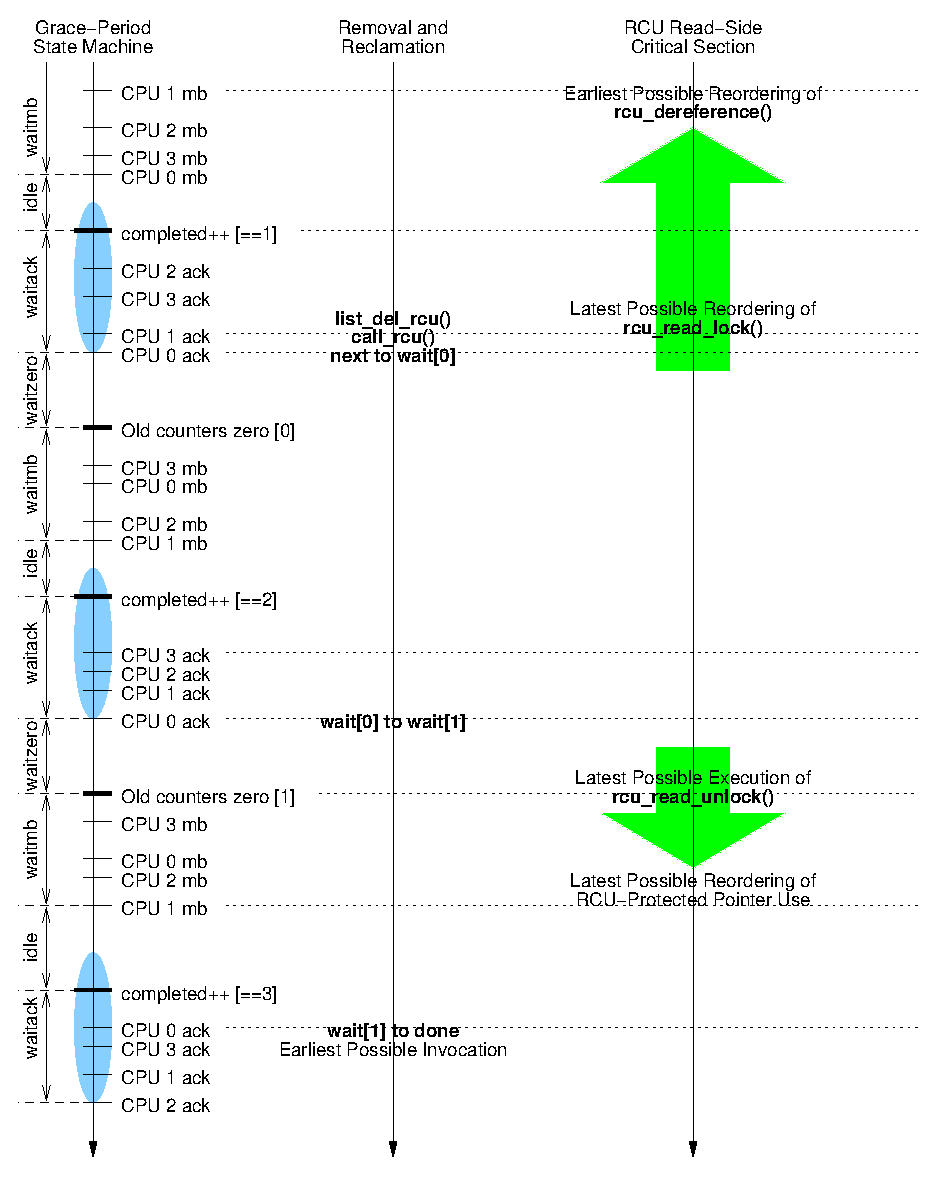
\includegraphics{appendix/rcuimpl/RCUpreemptValidation}}
\end{center}
\caption{Preemptible RCU Worst-Case Scenario}
\label{app:rcuimpl:Preemptible RCU Worst-Case Scenario}
\end{figure}

The worst-case scenario is shown in
Figure~\ref{app:rcuimpl:Preemptible RCU Worst-Case Scenario}.
Here, CPU~0 is executing the shortest possible
removal and reclamation sequence,
while CPU~1 executes the longest possible RCU read-side critical
section.
Because the callback queues are advanced just before acknowledging a
counter flip, the latest that CPU~0 can execute its
\co{list_del_rcu()} and \co{call_rcu()} is just before
its scheduling-clock interrupt that acknowledges the counter flip.
The \co{call_rcu()} invocation places the callback on CPU~0's
\co{next} list, and the interrupt will move the callback from
the \co{next} list to the \co{wait[0]} list.
This callback will move again (from the \co{wait[0]} list
to the \co{wait[1]} list) at CPU~0's first scheduling-clock
interrupt following the next counter flip.
Similarly, the callback will move from the \co{wait[1]} list
to the \co{done} list at CPU~0's first scheduling-clock
interrupt following the counter flip resulting in the value 3.
The callback might be invoked immediately afterward.

Meanwhile, CPU~1 is executing an RCU read-side critical section.
Let us assume that the \co{rcu_read_lock()} follows the first
counter flip (the one resulting in the value 1), so that the
\co{rcu_read_lock()} increments CPU~1's
\co{rcu_flipctr[1]} counter.
Note that because \co{rcu_read_lock()} does not contain any
memory barriers, the contents of the critical section might be executed
early by the CPU.
However, this early execution cannot precede the last memory barrier
executed by CPU~1, as shown on the diagram.
This is nevertheless sufficiently early that an \co{rcu_dereference()}
could fetch a pointer to the item being deleted by CPU~0's
\co{list_del_rcu()}.

Because the \co{rcu_read_lock()} incremented an index-1 counter,
the corresponding \co{rcu_read_unlock()} must
precede the ``old counters zero'' event for index 1.
However, because \co{rcu_read_unlock()} contains no memory
barriers, the contents of the corresponding RCU read-side critical
section (possibly including a reference to the item deleted by
CPU~0) can be executed late by CPU~1.
However, it cannot be executed after CPU~1's next memory barrier,
as shown on the diagram.
Because the latest possible reference by CPU~1 precedes the
earliest possible callback invocation by CPU~0, two passes
through the grace-period state machine suffice to constitute
a full grace period, and hence it is safe to do:

\vspace{5pt}
\begin{minipage}[t]{\columnwidth}
\small
\begin{verbatim}
    #define GP_STAGES 2
\end{verbatim}
\end{minipage}
\vspace{5pt}

\QuickQuiz{}
	Suppose that the irq disabling in
	\co{rcu_read_lock()} was replaced by preemption disabling.
	What effect would that have on \co{GP_STAGES}?
\QuickQuizAnswer{
	No finite value of \co{GP_STAGES} suffices.
	The following scenario, courtesy of Oleg Nesterov, demonstrates this:

	Suppose that low-priority Task~A has executed
	\co{rcu_read_lock()} on CPU 0,
	and thus has incremented \co{per_cpu(rcu_flipctr, 0)[0]},
	which thus has a value of one.
	Suppose further that Task~A is now preempted indefinitely.

	Given this situation, consider the following sequence of events:
	\begin{enumerate}
	\item	Task~B starts executing \co{rcu_read_lock()}, also on
		CPU 0, picking up the low-order bit of
		\co{rcu_ctrlblk.completed}, which is still equal to zero.
	\item	Task~B is interrupted by a sufficient number of scheduling-clock
		interrupts to allow the current grace-period stage to complete,
		and also be sufficient long-running interrupts to allow the
		RCU grace-period state machine to advance the
		\co{rcu_ctrlblk.complete} counter so that its bottom bit
		is now equal to one and all CPUs have acknowledged this
		increment operation.
	\item	CPU 1 starts summing the index==0 counters, starting with
		\co{per_cpu(rcu_flipctr, 0)[0]}, which is equal to one
		due to Task~A's increment.
		CPU 1's local variable \co{sum} is therefore equal to one.
	\item	Task~B returns from interrupt, resuming its execution of
		\co{rcu_read_lock()}, incrementing
		\co{per_cpu(rcu_flipctr, 0)[0]}, which now has a value
		of two.
	\item	Task~B is migrated to CPU 2.
	\item	Task~B completes its RCU read-side critical section, and
		executes \co{rcu_read_unlock()}, which decrements
		\co{per_cpu(rcu_flipctr, 2)[0]}, which is now -1.
	\item	CPU 1 now adds \co{per_cpu(rcu_flipctr, 1)[0]} and
		\co{per_cpu(rcu_flipctr, 2)[0]} to its
		local variable \co{sum}, obtaining the value zero.
	\item	CPU 1 then incorrectly concludes that all prior RCU read-side
		critical sections have completed, and advances to the next
		RCU grace-period stage.
		This means that some other task might well free up data
		structures that Task~A is still using!
	\end{enumerate}

	This sequence of events could repeat indefinitely, so that no finite
	value of \co{GP_STAGES} could prevent disrupting Task~A.
	This sequence of events demonstrates the importance of the promise
	made by CPUs that acknowledge an increment of
	\co{rcu_ctrlblk.completed}, as the problem illustrated by the
	above sequence of events is caused by Task~B's repeated failure
	to honor this promise.

	Therefore, more-pervasive changes to the grace-period state will be
	required in order for \co{rcu_read_lock()} to be able to safely
	dispense with irq disabling.
} \QuickQuizEnd

\QuickQuiz{}
	Why can't the \co{rcu_dereference()}
	precede the memory barrier?
\QuickQuizAnswer{
	Because the memory barrier is being executed in
	an interrupt handler, and interrupts are exact in the sense that
	a single value of the PC is saved upon interrupt, so that the
	interrupt occurs at a definite place in the code.
	Therefore, if the
	\co{rcu_dereference()} were to precede the memory barrier,
	the interrupt would have had to have occurred after the
	\co{rcu_dereference()}, and therefore
	the interrupt would also have had to have occurred after the
	\co{rcu_read_lock()} that begins the RCU read-side critical
	section.
	This would have forced the \co{rcu_read_lock()} to use
	the earlier value of the grace-period counter, which would in turn
	have meant that the corresponding \co{rcu_read_unlock()}
	would have had to precede the first ``Old counters zero [0]'' rather
	than the second one.
	This in turn would have meant that the read-side critical section
	would have been much shorter --- which would have been
	counter-productive,
	given that the point of this exercise was to identify the longest
	possible RCU read-side critical section.
} \QuickQuizEnd

\subsubsection{Formal Validation}
\label{app:rcuimpl:Formal Validation}

Formal validation of this algorithm is quite important, but remains
as future work.
One tool for doing this validation is described in
Section~\ref{chp:formal:Formal Verification}.

\QuickQuiz{}
	What is a more precise way to say ``CPU~0
	might see CPU~1's increment as early as CPU~1's last previous
	memory barrier''?
\QuickQuizAnswer{
	First, it is important to note that the problem with
	the less-precise statement is that it gives the impression that there
	might be a single global timeline, which there is not, at least not for
	popular microprocessors.
	Second, it is important to note that memory barriers are all about
	perceived ordering, not about time.
	Finally, a more precise way of stating above statement would be as
	follows: ``If CPU~0 loads the value resulting from CPU~1's
	increment, then any subsequent load by CPU~0 will see the
	values from any relevant stores by CPU~1 if these stores
	preceded CPU~1's last prior memory barrier.''

	Even this more-precise version leaves some wiggle room.
	The word ``subsequent'' must be understood to mean ``ordered after'',
	either by an explicit memory barrier or by the CPU's underlying
	memory ordering.
	In addition, the memory barriers must be strong enough to order
	the relevant operations.
	For example, CPU~1's last prior memory barrier must order stores
	(for example, \co{smp_wmb()} or \co{smp_mb()}).
	Similarly, if CPU~0 needs an explicit memory barrier to
	ensure that its later load follows the one that saw the increment,
	then this memory barrier needs to be an \co{smp_rmb()}
	or \co{smp_mb()}.

	In general, much care is required when proving parallel algorithms.
} \QuickQuizEnd

